% Standalone volume. Compile with pdfLaTeX (repeat for references and contents).
% All eight manuscripts, illustrations, and bibliographic data are inline.
\documentclass[11pt,a4paper,oneside,openany]{report}
\usepackage[T1]{fontenc}
\usepackage{lmodern,amsmath,amssymb,amsthm,booktabs,array,tikz,fancyhdr}
\usepackage[left=24mm,right=24mm,top=23mm,bottom=24mm]{geometry}
\definecolor{ink}{HTML}{153F45}
\definecolor{sea}{HTML}{53A89D}
\usepackage[bookmarksopen=true,bookmarksopenlevel=0,bookmarksnumbered=true,colorlinks=true,linkcolor=ink,citecolor=ink,urlcolor=ink]{hyperref}
\hypersetup{pdftitle={Euler's Constant, Stieltjes Constants, and Harmonic Denominators},pdfauthor={Research notes prepared for Keio},pdfsubject={Collected research papers on arithmetic approximation, lattice counts and harmonic sums},pdfdisplaydoctitle=true}
\newtheorem{theorem}{Theorem}[section]
\newtheorem{lemma}[theorem]{Lemma}\newtheorem{proposition}[theorem]{Proposition}
\newtheorem{corollary}[theorem]{Corollary}
\theoremstyle{remark}\newtheorem{remark}[theorem]{Remark}
\numberwithin{equation}{section}
\newcommand{\ee}{\mathrm e}\newcommand{\E}{\mathbb E}\newcommand{\V}{\mathcal V}
\newcommand{\EE}{\mathbb E}\newcommand{\T}{\mathbb R/\mathbb Z}
\newcommand{\A}{\overline{\mathbb Q}}\newcommand{\B}{\mathcal B}
\newcommand{\Z}{\mathbb Z}\newcommand{\N}{\mathbb N}
\newcommand{\dens}{\overline d}\newcommand{\lcm}{\operatorname{lcm}}
\newcommand{\card}{\#}\newcommand{\vol}{\operatorname{meas}}
\setlength{\headheight}{15pt}\setlength{\emergencystretch}{2.8em}
\setcounter{tocdepth}{1}\setcounter{secnumdepth}{2}
\pagestyle{fancy}\fancyhf{}\fancyhead[L]{\small\itshape\nouppercase{\leftmark}}
\fancyfoot[C]{\thepage}
\renewcommand{\chaptermark}[1]{\markboth{\thechapter\enspace\textperiodcentered\enspace #1}{}}
\renewcommand{\headrulewidth}{.3pt}
\fancypagestyle{plain}{\fancyhf{}\fancyfoot[C]{\thepage}\renewcommand{\headrulewidth}{0pt}}
\makeatletter
\renewcommand{\@makechapterhead}[1]{\vspace*{4pt}{\parindent\z@\raggedright
 {\normalfont\small\sffamily\bfseries\color{ink}\MakeUppercase{\@chapapp}\enspace\thechapter\par}
 \vspace{9pt}{\normalfont\color{ink}\huge\bfseries #1\par}\nobreak\vspace{13pt}}}
\renewcommand{\@makeschapterhead}[1]{\vspace*{4pt}{\parindent\z@\raggedright
 \normalfont\color{ink}\huge\bfseries #1\par}\nobreak\vspace{15pt}}
\makeatother
\renewcommand{\bibname}{References}
\raggedbottom
\begin{document}
\pagenumbering{roman}
\pdfbookmark[0]{Title and reading guide}{volume-title}
\thispagestyle{empty}
\vspace*{18mm}
{\noindent\small\sffamily\bfseries\color{ink} COLLECTED RESEARCH PAPERS\par}
\vspace{6mm}
{\noindent\raggedright\fontsize{28}{34}\selectfont\bfseries\color{ink}
Euler's Constant,\\[2pt] Stieltjes Constants,\\[2pt] and Harmonic Denominators\par}
\vspace{4mm}
{\noindent\large Rational approximation, lattice counts, and prime cancellation\par}
\vspace{7mm}
{\noindent Prepared for Keio\quad\textperiodcentered\quad 21 November 2026\par}
\vspace{11mm}
\noindent\rule{\textwidth}{.5pt}\par\vspace{2mm}
\noindent\textbf{Reading guide}\par\smallskip
\noindent Three questions connect the eight papers in this volume.
\begin{description}
\item[How small are the reduced linear forms?] Chapters~\ref{chap:1}--\ref{chap:3} study the effect of exact logarithm cancellation, signed errors, and denominator growth on rational approximation to Euler's constant. Chapter~\ref{chap:1} also treats the Euler--Gompertz constant.
\item[What can a lattice count or a progression recover?] Chapters~\ref{chap:4} and~\ref{chap:5} turn the area of a folded hyperbola into finite grid counts and determine the resolution needed by a particular statistic. Chapters~\ref{chap:6} and~\ref{chap:7} pass to arithmetic progressions, prove transcendence and rank results for families of Stieltjes constants, and recover expressions involving the original $\gamma$.
\item[How often do harmonic denominators lose primes?] Chapter~\ref{chap:8} gives an unconditional proof of the Wu--Yan upper-density conclusion and establishes simultaneous prime divisibility throughout long intervals.
\end{description}
\vfill
\noindent\textit{Scope.} The irrationality of $\gamma$ remains open in this collection. Each chapter retains its hypotheses, proofs, and finite certificates. Chapter and section numbers, cross-references, and the bibliography are shared throughout the volume.
\clearpage
\pdfbookmark[0]{Contents}{volume-contents}
\tableofcontents\clearpage
\pagenumbering{arabic}

% ===== Source 1: Euler_Constants_Approximation.tex =====
\chapter[Approximation for two Euler constants]{Logarithm cancellation and primitive approximation for two Euler constants}\label{chap:1}
\noindent\textbf{Abstract.}\enspace We study two attempts to prove irrationality at the original values of Euler's constant and the Euler--Gompertz constant.
For Sondow's integrals, we prove that the minimum width of a block beginning at $N$ that admits exact rational cancellation of its logarithms is of order $N/\log N$. For arbitrary support we also give a lower bound on its cardinality. It implies transcendence of all but finitely many strictly nested quotients of normalized integral differences. On blocks of the critical order we also obtain small integer coefficients, although the resulting signed remainder can vanish identically.
For the Euler--Gompertz constant, we prove a quadratic gap between indices at which the classical, fully reduced Laguerre linear forms are bounded. For each fixed bound their number below $X$ is at most $(\log\log X)/\log 2+O(1)$. Near-quadratic pairs satisfy a further iterated-logarithm bound. An infinite bounded subsequence would yield simultaneous Liouville approximation to six values of Euler's factorial series in different completions. The individual irrationality of both real constants remains open.

\section{The two irrationality questions}
The named targets are
\[
 \gamma=\lim_{n\to\infty}\left(\sum_{k=1}^n\frac1k-\log n\right),
 \qquad
 \delta=\int_0^\infty \frac{e^{-t}}{1+t}\,dt .
\]
At least one of these numbers is transcendental \cite{lagarias}. Identifying either specific number as irrational would answer a separate longstanding question. Sondow's criteria \cite{sondow} and the work of Murabayashi and Yoshida \cite{my} give concrete ways to approach the respective questions.

Both constructions seek a sequence of nonzero numbers $a_n\xi-b_n$ tending to zero with $a_n,b_n\in\mathbb Z$. If $\xi=u/v\in\mathbb Q$ with $v>0$, every such number has absolute value at least $1/v$. For $\gamma$, the obstruction is to retain a nonzero signed error after logarithms have been cancelled. For $\delta$, the classical remainders are positive, and the issue is the size of the error after division by the full common divisor. We keep the original target in each construction and investigate the index sets on which these two requirements could hold.

\section{The width needed to cancel Sondow's logarithms}
\label{ch1:so:section}

Let $H_0=0$, $H_m=\sum_{i=1}^m1/i$, and
$D_m=\operatorname{lcm}(1,\ldots,m)$. Sondow's integral evaluation
\cite{sondow} gives
\begin{align}
 I_n&=\int_0^1\!\int_0^1
 \frac{[x(1-x)y(1-y)]^n}{(1-xy)(-\log(xy))}\,dx\,dy
 =C_n\gamma-A_n+\Lambda_n, \label{ch1:so:identity}\\
 C_n&=\binom{2n}{n},\qquad A_n=\sum_{i=0}^n\binom ni^2 H_{n+i},\nonumber\\
 \Lambda_n&=\sum_{k=1}^n b_{n,k}\log(n+k),\qquad
 b_{n,k}=2\sum_{i=0}^{\min(k-1,n-k)}
          \binom ni^2(H_{n-i}-H_i).\label{ch1:so:weights}
\end{align}
Each $\Lambda_n$ is a rational linear combination of prime logarithms.
Since $D_{2n}\Lambda_n=\log S_n$ for Sondow's positive integer $S_n$, rational
linear dependence among a block of $\Lambda_n$ is equivalent to multiplicative
dependence among the corresponding $S_n$.

The corpus manuscript \cite{vm19} establishes the rank $\pi(2M)$ on
the prefix $1,\ldots,M$, rules out a fixed polynomial-coefficient
recurrence, and constructs short relations on blocks of positive
relative width. Manuscript \cite{vm105} obtains a prime-band width bound for a different family of proper rational kernels. Here the varying harmonic weights in \eqref{ch1:so:weights} require a zero estimate for Sondow's original coefficients. Prefix rank permits the first coordinates of a relation
to stay fixed as $M$ increases. A different question asks how wide a block
starting at an arbitrarily prescribed late index must be to contain
\emph{any} relation. Define
\[
 w_N=\min\{d\geq 0:\ \Lambda_N,\ldots,\Lambda_{N+d}
                   \text{ are linearly dependent over }\mathbb Q\}.
\]
The endpoints of the support of a relation may lie inside the block.

\begin{theorem}\label{ch1:so:width}
The width $w_N$ is finite for every $N\geq1$ and satisfies
\[
 \frac1{240}\leq\liminf_{N\to\infty}\frac{w_N\log N}{N}
 \leq\limsup_{N\to\infty}\frac{w_N\log N}{N}\leq 2 .
\]
In particular the order of the least width is $N/\log N$. The constants
in these bounds need not be optimal.
\end{theorem}

The lower bound uses all prime coordinates in an interval.
Their coefficients extend to functions of an integer variable. Two
successive differences, with a rational normalization between them, bound
the number of integer zeros of every nonzero linear combination.

\begin{lemma}\label{ch1:so:zeros}
Let $N\geq 2$ and $0\le d\le N/40$ be integers. For $0\le j\le d$ define
\[
 W_j(u)=2\sum_{i=0}^{u+2j}\binom{N+j}{i}^{\!2}
        (H_{N+j-i}-H_i),\qquad
 0\le u\le \left\lfloor (N-3d-1)/2\right\rfloor .
\]
If $c_0,\ldots,c_d$ are real and not all zero, the function
$F(u)=\sum_{j=0}^d c_jW_j(u)$ has at most $120d+24$ integer zeros on
$1\le u\le\lfloor(N-3d-1)/2\rfloor$.
\end{lemma}

\begin{proof}
Write $(v)_j=v(v+1)\cdots(v+j-1)$ and
$v^{\underline j}=v(v-1)\cdots(v-j+1)$, with both empty products equal
to one. For $1\le u\le\lfloor(N-3d-1)/2\rfloor$, put
\begin{align*}
 h(u)&=H_{N-u}-H_u,\\
 r_j(u)&=\frac{(N+1)_j(N-u)^{\underline j}}{(u+1)_{2j}},\\
 t_j(u)&=\sum_{i=0}^{j-1}\frac1{N-u-i}
              +\sum_{i=1}^{2j}\frac1{u+i}.
\end{align*}
With $D(u)=(u+1)_{2d}^{\,3}$, the last term in the sum for $W_j$ gives
\begin{align*}
 \frac{F(u)-F(u-1)}{2\binom Nu^2}
 &=\sum_{j=0}^d c_jr_j(u)^2\{h(u)-t_j(u)\}\\
 &=\frac{P(u)h(u)+Q(u)}{D(u)} .
\end{align*}
Indeed $r_j(u)=\binom{N+j}{u+2j}/\binom Nu$ and
$H_{N-u-j}-H_{u+2j}=h(u)-t_j(u)$.
The polynomials $P=D\sum c_j r_j^2$ and
$Q=-D\sum c_jr_j^2t_j$ have degrees at most $6d$. Each denominator
$N-u-i$ in $t_j$ divides the numerator of $r_j$. The other
denominators divide $(u+1)_{2j}$. The degree bound follows also from
$r_j=O(u^{-j})$ and $t_j=O(u^{-1})$ at infinity.
For the largest index $j>0$ with $c_j\ne0$, the summand $c_jr_j^2$
has a double pole at $-2j$ shared by no earlier summand. If the last
index is zero then $\sum c_jr_j^2=c_0$. Thus $P\ne0$ in both cases.

Let $V=Q/P$. Away from poles set $T(u)=h(u)+V(u)$ on the integer
grid. Its forward difference there is the restriction of
\[
 U(z)=-\frac1{N-z}-\frac1{z+1}+V(z+1)-V(z).
\]
Multiplication by $(N-z)(z+1)P(z+1)P(z)$ gives a polynomial of degree
at most $12d+2$. This polynomial is nonzero. If $U$ vanished
identically, the residues $a_k$ of $V$ at the integers would satisfy
\[
 a_{k+1}-a_k=\mathbf 1_{\{k=-1\}}-\mathbf 1_{\{k=N\}} .
\]
Only finitely many $a_k$ can be nonzero. Summing the displayed
relation from the left gives $a_0=\cdots=a_N=1$, requiring at least
$N+1$ poles although $\deg P\le6d<N+1$.

Cut the real line at the real roots of $P(z)$, $P(z+1)$, the
numerator just obtained for $U$, and the points $-1,N$. There are
at most $s=24d+4$ cuts. On each complementary interval $P$ and $U$
have fixed nonzero sign. At consecutive integer points of its
intersection with the stated grid, $T$ is strictly monotone. Since
$D$ and $\binom Nu^2$ are positive on the grid, the backward
differences of $F$ have the signs of $P(u)T(u)$. On the interval they
therefore split into at most two runs of strict sign and at most one
isolated zero. The values of $F$ have at most four zeros there:
along each run the values are strictly monotone, and one zero
difference can contribute one extra grid point. This bound also
covers single-point intervals. Each cut itself contributes at most
one integer zero. The total is at most $4(s+1)+s\le120d+24$.
\end{proof}

\begin{proof}[Proof of Theorem~\ref{ch1:so:width}]
The block from $N$ to $N+d$ uses at most $\pi(2(N+d))$ prime logarithms.
The prime number theorem implies that $d+1>\pi(2(N+d))$ eventually
for fixed $N$ as $d\to\infty$. It also gives this inequality for
$d=\lceil(2+\epsilon)N/\log N\rceil$ as $N\to\infty$, for each
fixed $\epsilon>0$. Rational dimension gives the finiteness and the
upper bound.

For the lower bound fix $0<\kappa<1/240$ and take
$d=\lfloor\kappa N/\log N\rfloor$, so $d\le N/40$ eventually.
If $p$ is a prime in
\[
 \frac{3(N+d)+1}{2}\le p\le 2N-1,\qquad u=2N-p,
\]
then $u$ belongs to the grid in Lemma~\ref{ch1:so:zeros}. For every
$n=N+j$, $0\le j\le d$, the only multiple of $p$ among
$n+1,\ldots,2n$ is $p$. At $k=p-n$, the minimum in
\eqref{ch1:so:weights} is $n-k=2n-p=u+2j$, since $2p\ge3n+1$.
Thus $W_j(u)$ is exactly the coefficient of $\log p$ in $\Lambda_{N+j}$.
A rational linear relation would force $F(2N-p)=0$ for every such
prime, by unique factorization after clearing rational denominators.
The prime number theorem counts $(\tfrac12+o(1))N/\log N$ of these
primes. Lemma~\ref{ch1:so:zeros} allows at most
$(120\kappa+o(1))N/\log N$ zeros. Since $120\kappa<1/2$, a
nontrivial relation is impossible for all sufficiently large $N$.
Letting $\kappa$ tend to $1/240$ proves the result.
\end{proof}

\subsection{Height control at the same order of width}

\begin{proposition}\label{ch1:so:height}
Fix $\eta>0$ and $K>2+2(1+\log4)/\eta$. For all sufficiently large
$N$, put $M=N+\lceil K N/\log N\rceil$. There exists a nonzero
integer vector $(c_n)_{N\le n\le M}$ with
\begin{align}
 &\max_n |c_n|\le e^{\eta N},\qquad \sum_{n=N}^M c_n \Lambda_n=0,
 \label{ch1:so:heightconditions}\\
 &D_{2M}\sum_{n=N}^M |c_n| I_n
 \le \exp\{-(\log16-2-\eta)N+o(N)\}. \label{ch1:so:error}
\end{align}
The vector may additionally be required to satisfy
$\sum c_n C_n=\sum c_n A_n=0$.
\end{proposition}

\begin{proof}
There are $s=M-N+1$ columns and $r=\pi(2M)$ prime rows. Multiply
the prime coefficients of every $\Lambda_n$ by $D_M$. The result is
integral by \eqref{ch1:so:weights}, since the harmonic numbers in
$b_{n,k}$ have indices at most $M$. Vandermonde's binomial identity
gives $b_{n,k}\le2H_n4^n$, and $v_p(n+k)\le\log_2(2M)$.
Consequently the prime-row entries have absolute value at most
\[
 H=\left\lceil 2M H_M 4^M D_M \log_2(2M)\right\rceil ,
 \qquad \log H=(1+\log4+o(1))N.
\]
Here we used $\log D_m=m+o(m)$, another form of the prime number
theorem. Append the two integer rows $C_n,D_{2M}A_n$. Their entries
are bounded by $H'=\lceil 4^M D_{2M}H_{2M}\rceil$, with
$\log H'=O(N)$.

Take $B=\lfloor e^{\eta N}\rfloor$. On the grid $\{0,\ldots,B\}^s$
the number of images of the resulting integer matrix is at most
$(2sHB+1)^r(2sH'B+1)^2$. Its logarithm is at most
\[
 \bigl(2(1+\log4+\eta)+o(1)\bigr)N^2/\log N ,
\]
whereas the logarithm of the number of grid points is
$(K\eta+o(1))N^2/\log N$. The strict inequality on $K$ therefore
gives two different grid points with the same image. Their difference
proves \eqref{ch1:so:heightconditions} and both additional equations.
Finally $I_n\le I_1 16^{-(n-1)}$ by the integral in
\eqref{ch1:so:identity}. Summing the absolute contributions and using
$\log D_{2M}=2N+o(N)$ proves \eqref{ch1:so:error}.
\end{proof}

For instance, $\eta=2/3$ and $K=10$ give an exponentially decaying
bound in \eqref{ch1:so:error}. This proves that exact logarithm
elimination with an exponentially small absolute error budget is
possible already at width $O(N/\log N)$, and Theorem~\ref{ch1:so:width}
rules it out at width $o(N/\log N)$.
For a vector satisfying \eqref{ch1:so:heightconditions}, the signed
quantity $D_{2M}\sum c_nI_n$ belongs to $\mathbb Z+\mathbb Z\gamma$.
If $\gamma=a/b$ were rational, every nonzero such quantity would
have absolute value at least $1/b$. The extra equations in
Proposition~\ref{ch1:so:height} explicitly allow the signed quantity
to vanish. An irrationality proof by this construction still requires
nonzero signed values along an unbounded sequence of blocks.

\subsection{Linear independence for normalized integral differences}
Write $Y_n=I_n/C_n$. Corpus manuscript \cite{vm170} treats individual differences and their spans on prefixes. The width estimate gives a simultaneous result on every sufficiently late block, including blocks whose length grows with their starting index.

\begin{corollary}\label{ch1:so:chords}
For any $N$ and $1\le d<w_N$, the $d+1$ real numbers
\[
 1,\quad Y_{N+1}-Y_N,\quad \ldots,\quad Y_{N+d}-Y_N
\]
are linearly independent over $\overline{\mathbb Q}$. This holds for all sufficiently large $N$ and all $1\le d\le \kappa_0 N/\log N$, for every fixed $0<\kappa_0<1/240$.
\end{corollary}
\begin{proof}
Let $b_j$ be the vector of rational prime coefficients of $\Lambda_{N+j}/C_{N+j}$, $0\le j\le d$. The definition of $w_N$ and unique factorization give full column rank over $\mathbb Q$. A nonzero rational minor remains nonzero over $\overline{\mathbb Q}$, so $b_1-b_0,\ldots,b_d-b_0$ are independent over this field.
By \eqref{ch1:so:identity} each $Y_{N+j}-Y_N$ is a rational number plus the scalar product of $b_j-b_0$ with the vector of prime logarithms. The inhomogeneous form of Baker's theorem gives linear independence of $1$ and those prime logarithms over $\overline{\mathbb Q}$ \cite{baker}. Any putative relation therefore forces all prime coordinates of its linear combination to vanish. Independence of the difference vectors forces all its difference coefficients to vanish, and the constant coefficient follows. The last assertion follows from Theorem~\ref{ch1:so:width}.
\end{proof}
For example, every nonzero algebraic linear combination of the $d$ displayed differences is transcendental. The cancellation that makes this possible also removes $\gamma$ from each difference.

\paragraph{Finite checks of the exact width.}
The defining matrix permits checks without numerical logarithms. The following are exact finite ranks.
\[
\begin{array}{c|rrrrrr}
 N&8&16&32&64&128&256\\ \hline
 w_N&12&19&30&47&80&137
\end{array}
\]
Here is a reproducible rank certificate procedure for each column of the table. Set $d$ equal to the tabulated width; form the rows for $p\le2(N+d)$ using
$M_{p,n}=\sum_{k=1}^n b_{n,k}v_p(n+k)$ from \eqref{ch1:so:weights}. Row reduction of the columns $n=N,\ldots,N+d-1$ modulo $1000003$ gives rank $d$. The integers occurring as denominators in the harmonic sums are all smaller than this prime. There are exactly $d$ primes at most $2(N+d)$ in each of the six cases. Thus the first $d$ columns are independent over $\mathbb Q$ and adjoining one more forces dependence.

\subsection{Relations on nonconsecutive indices}
The width of the support and the number of its nonzero coefficients measure different restrictions. The same zero estimate controls the latter, even if there are arbitrarily large gaps between the indices.

\begin{theorem}\label{ch1:so:sparse}
Fix $0<\nu<13/30$. For all sufficiently large $M$, every rational relation amongst the $\Lambda_n$ with largest nonzero index $M$ uses more than
\[
 \nu\frac{\log M}{\log\log M}
\]
nonzero coefficients.
\end{theorem}
\begin{proof}
Choose $17/30<\theta<1-\nu$. The short-interval prime number theorem of Guth and Maynard \cite[Corollary 1.3]{gm} implies the following uniform bound for large $M$. An interval of length $T-1$, with endpoints $2M+o(M)$ and $M^\theta\le T=o(M)$, contains at least $T/(3\log M)$ primes. For the full range of $T$, take $17/30<\tau<\min(\theta,0.99)$. Tile the interval by intervals of length $M^\tau$, leaving a final remainder of smaller length. The cited asymptotic applies uniformly to the full intervals since their left endpoints are asymptotic to $2M$. The remainder is $o(T)$, giving the stated lower bound.

Suppose the relation has $k\le\nu\log M/\log\log M$ terms. Start with its last term and successively adjoin the next earlier term. At any stage let $N$ be the least of the selected indices and $d=M-N$. The selected terms are precisely the terminal part of the relation. With an absolute constant $K=1000$ put
\[
 T=\left\lceil K\big((d+1)\log M+M^\theta\big)\right\rceil .
\]
As long as $d,T=o(M)$, all primes $p\in(2N-T,2N-1]$ are eligible for the coefficient formula used in Lemma~\ref{ch1:so:zeros}, with starting index $N$ and width $d$. In fact $d\le N/40$ and $p\ge (3M+1)/2$ for large $M$. This interval contains more than $120d+24$ primes. If there is no earlier term, or if the next earlier index $n'$ satisfies $2n'\le2N-T$, those primes occur only in the selected columns. The coefficient of each of their logarithms must be zero. This would give more zeros of the nontrivial terminal combination than Lemma~\ref{ch1:so:zeros} permits.

Consequently a next term must exist, with its new width $d'=M-n'<d+T$. For some fixed $C$,
\[
 d'+M^\theta\le C\log M\,(d+M^\theta).
\]
The size assumptions used in this argument hold uniformly at every stage. Indeed, starting with $d=0$, after at most $k$ applications the inductive upper bound is
\[
 M^\theta(C\log M)^k\le M^{\theta+\nu+o(1)}.
\]
Its exponent is strictly below one, even after the extra factor $O(\log M)$ used in $T$. Once all $k$ terms have been selected, the same argument still requires another, a contradiction.
\end{proof}

This gives a value-transcendence consequence on nested intervals. Manuscript \cite{vm170} gives a criterion for all chord quotients and settles those with correspondingly ordered endpoints. For $a<b<c<d$ consider the strictly nested quotient
\[
 Z_{a,b,c,d}=\frac{Y_a-Y_d}{Y_b-Y_c}.
\]
The positive integral $I_n$ decreases strictly and $C_n$ increases, so the denominator is nonzero.
\begin{corollary}\label{ch1:so:nested}
There is an absolute $d_0$ such that $Z_{a,b,c,d}$ is transcendental for every $1\le a<b<c<d$ with $d\ge d_0$.
\end{corollary}
\begin{proof}
If $Z_{a,b,c,d}$ were algebraic, the identity defining it would express zero as an algebraic linear combination of $1$ and the prime logarithms. Baker's theorem forces every prime coefficient to vanish. In the resulting relation among the four rational columns of prime coefficients of $\Lambda_j/C_j$ the coefficient at $d$ is $-1$. A consistent rational linear system with this last coefficient fixed to $-1$ has a rational solution, by elimination. Undoing the rational column scalings would give a rational relation with last index $d$ and at most four nonzero coefficients, contrary to Theorem~\ref{ch1:so:sparse} for all sufficiently large $d$.
\end{proof}

\section{The Laguerre approximants to the original constant}
\label{ch1:sec:gomp-family}

We now turn to the real Euler--Gompertz constant
\[
  \delta=\int_0^\infty\frac{e^{-x}}{1+x}\,dx.
\]
The classical Laguerre approximants occur in the continued fraction for
this integral \cite{lagarias,ems}. Its individual irrationality is open
in the sources \cite{my,ems}. Define integer sequences by
\[
 (Q_0,P_0)=(1,0),\quad (Q_1,P_1)=(2,1),\qquad
 U_{n+1}=2(n+1)U_n-n^2 U_{n-1}\quad(n\ge1).
\]
Put
\[
 \begin{gathered}
 R_n=Q_n\delta-P_n,\qquad g_n=\gcd(Q_n,P_n),\qquad
 (q_n,p_n)=(Q_n/g_n,P_n/g_n),\\
 L_n=R_n/g_n,\qquad e_n=R_n/Q_n .
 \end{gathered}
\]
In particular $L_n=q_n e_n$ and $P_n/Q_n=p_n/q_n$. The question about
this method is whether $L_{n_j}\to0$ along any infinite sequence. Since
each $L_n>0$, such a sequence would prove $\delta$ irrational.

\subsection{An elementary bound for the relative error}

Let $\pi_n(x)=(-1)^n e^x(d/dx)^n(e^{-x}x^n)$ be the monic Laguerre
polynomial. Its three-term recurrence is
$\pi_{n+1}=(x-2n-1)\pi_n-n^2\pi_{n-1}$. Set
\[
 B_n(z)=z^n\pi_n(1/z)
       =\sum_{j=0}^n(-1)^j j!\binom nj^2 z^j,\quad
 A_n(z)=\int_0^\infty e^{-x}
          \frac{B_n(z)-z^n\pi_n(x)}{1-zx}\,dx.
\]
The quotient in the integral is polynomial in $x,z$ after cancellation.
The recurrence for $\pi_n$ gives
$U_{n+1}=(1-(2n+1)z)U_n-n^2z^2U_{n-1}$ for $B_n,A_n$ when
$n\ge1$. For the latter sequence the additional term is proportional
to $\int e^{-x}\pi_n(x)\,dx=0$ over the positive half-line.
The initial values then give $B_n(-1)=Q_n$ and $A_n(-1)=P_n$.
Rodrigues's formula and $n$ integrations by parts give
\begin{equation}\label{ch1:eq:gomp-raw}
  R_n=n!\int_0^\infty\frac{e^{-x}x^n}{(1+x)^{n+1}}\,dx>0.
\end{equation}
The boundary terms vanish because $e^{-x}x^n$ has a zero of order $n$
at zero and all its derivatives decay at infinity. In particular,
$0<P_n/Q_n<\delta<1$ for $n\ge1$, where positivity of $P_n/Q_n$
also follows from the determinant below.

Write $W_{n,m}=Q_nP_m-P_nQ_m$. The recurrence gives
\begin{equation}\label{ch1:eq:gomp-wronskian}
 W_{n,n+1}=(n!)^2,\qquad
 (n!)^2\mid W_{n,m}\quad(m>n).
\end{equation}
Indeed $W_{0,1}=1$ and $W_{n,n+1}=n^2 W_{n-1,n}$. For fixed $n$
the second statement follows by applying the recurrence in $m$,
starting at $W_{n,n}=0$. Thus the approximants increase strictly.
The identity for $B_n$ also gives
\[
  Q_n=n!\sum_{k=0}^n \binom nk/k!
  \le n!\sum_{k\ge0}\frac{n^k}{(k!)^2}\le n!e^{2\sqrt n}.
\]
The last sum is bounded by the square of $\sum_{k\ge0}(\sqrt n)^k/k!$.
Since $P_{m+1}/Q_{m+1}<\delta$, we obtain
\begin{equation}\label{ch1:eq:gomp-relative}
 e_m>\frac{(m!)^2}{Q_mQ_{m+1}}
 \ge\frac{\exp(-2\sqrt m-2\sqrt{m+1})}{m+1}.
\end{equation}

\section{A quadratic gap after full gcd reduction}
\label{ch1:sec:gomp-gap}

The corpus gives modular reset identities \cite{vm33} and an
$O_B(\log X)$ bound for the number of $n\le X$ with $L_n\le B$
\cite{vm30}. We retain the full reduced denominators and estimate
the determinant at two arbitrary indices. Let
\[
 \begin{gathered}
 S=\{2,3,5,13,23,41\},\qquad
 s=\sum_{p\in S}\frac{\log p}{p-1},\\
 D_n=\tfrac14\prod_{p\in S}p^{2v_p(n!)},\qquad
 \kappa=s^2/4=1.09612560679958\ldots .
 \end{gathered}
\]
All logarithms are natural.

\begin{lemma}\label{ch1:lem:gomp-primes}
For $p\in S\setminus\{2\}$, every $Q_n$ is a $p$-adic unit.
For $p=2$, $Q_{2k}$ is odd and $Q_{2k+1}\equiv2\pmod4$.
\end{lemma}
\begin{proof}
In $Q_n=\sum_{j=0}^n j!\binom nj^2$, the summands with $j\ge p$
vanish modulo $p$. For $j<p$, the binomial coefficient depends
modulo $p$ only on $n\bmod p$. Thus it suffices to test $0\le n<p$.
The entries of the second row are the least nonnegative residues
of the indicated product.
\[
\begin{array}{c|rrrrr}
 p&3&5&13&23&41\\ \hline
 \prod_{r=0}^{p-1}Q_r\pmod p&2&4&11&18&6
\end{array}
\]
For an explicit reproduction, initialize $(a,b,c)=(1,2,2)$.
For $j=1,\ldots,p-2$, replace $(a,b)$ by
$(b,2(j+1)b-j^2a)$ modulo $p$, then replace $c$ by $cb\bmod p$
using the new $b$. The final $c$ gives the table.
For $p=2$, the recurrence gives $Q_{2k}\equiv Q_{2k-2}\pmod2$
for $k\ge1$ and $Q_{2k+1}\equiv2Q_{2k}\pmod4$ for $k\ge1$; $Q_1=2$ supplies the initial odd index.
\end{proof}

\begin{theorem}\label{ch1:thm:gomp-gap}
For every pair $1\le n<m$,
\begin{equation}\label{ch1:eq:gomp-master}
  L_nL_m>D_n e_m>
  \frac{D_n}{m+1}\exp(-2\sqrt m-2\sqrt{m+1}).
\end{equation}
Fix $B>0$. If $n<m$ range over pairs with $L_n,L_m\le B$ and
$n\to\infty$, then $\liminf m/n^2\ge\kappa$. In particular,
\begin{equation}\label{ch1:eq:gomp-count}
 \#\{1\le n\le X:L_n\le B\}
 \le \frac{\log\log X}{\log 2}+O_B(1)
 \qquad(X\ge3).
\end{equation}
\end{theorem}
\begin{proof}
The reduced determinant $W_{n,m}/(g_ng_m)$ is a positive integer.
At odd primes of $S$, neither content is divisible by the prime.
At $2$ each content has valuation at most one. By
\eqref{ch1:eq:gomp-wronskian} the reduced determinant is therefore at
least $D_n$ (if its prescribed exponent at $2$ is negative the
inequality still holds). On the other hand
\[
 0<W_{n,m}=Q_mR_n-Q_nR_m<Q_mR_n.
\]
Consequently $L_n L_m/e_m=R_n Q_m/(g_ng_m)>D_n$.
Equation~\eqref{ch1:eq:gomp-relative} proves the remaining inequality.

Legendre's formula gives $\log D_n=2sn+O(\log(n+1))$ for this fixed
set $S$. For the specified pairs,
\[
 2sn\le 2\sqrt m+2\sqrt{m+1}+\log(m+1)+2\log B+O(\log(n+1)).
\]
Along any subsequence on which $m/n^2$ is bounded, division by $n$
gives $\liminf\sqrt m/n\ge s/2$; unbounded ratios cannot decrease
the lower limit through a finite cluster point. Since $\kappa>1$,
every sufficiently late pair satisfies $m\ge n^2$. Starting from any
fixed sufficiently large exceptional index $n_0>1$, the $j$th subsequent
index is at least $n_0^{2^j}$. Taking logarithms twice gives
\eqref{ch1:eq:gomp-count}, also when there are only finitely many such indices.
\end{proof}

\section{What a bounded real subsequence would imply at six primes}
\label{ch1:sec:gomp-padic}

Let $F_p=\sum_{k\ge0}(-1)^kk!\in\mathbb Z_p$. The common formal
Pad\'e approximants for the real Hardy integral and Euler's factorial
series are classical \cite{mz,ems}. Their simultaneous specialization
here yields an additional necessary condition.
For any prime $p$, normalize $|p|_p=p^{-1}$. For a reduced fraction
$a/b$ its height is $H(a/b)=\max(|a|,|b|)$. Call $y\in\mathbb Q_p$
Liouville if for every $d>0$ there are infinitely many distinct rational
$x$ with $0<|x-y|_p<H(x)^{-d}$.

\begin{theorem}\label{ch1:thm:gomp-padic}
If $(L_n)$ has an infinite bounded subsequence, every $F_p$ for
$p\in S$ is a $p$-adic Liouville number. The same rational approximants
work simultaneously at these six places. In particular, if one of
the six values fails to be Liouville, then $L_n\to+\infty$.
\end{theorem}
\begin{proof}
As a formal series at $z=0$ one has
\begin{equation}\label{ch1:eq:gomp-formal}
 B_n(z)\sum_{k\ge0}k!z^k-A_n(z)
 =(n!)^2z^{2n}\sum_{h\ge0} h!\binom{n+h}{n}^2 z^h.
\end{equation}
Indeed the left side is the formal moment integral of
$z^n\pi_n(x)/(1-zx)$ against $e^{-x}\,dx$ on $[0,\infty)$.
By Rodrigues's formula its $x^k$ moment without $z^n$ is zero for
$k<n$, and $(k!)^2/(k-n)!$ for $k\ge n$.
All series in \eqref{ch1:eq:gomp-formal} converge $p$-adically at $z=-1$,
so
\[
 v_p(F_p-P_n/Q_n)\ge 2v_p(n!)-v_p(Q_n).
\]
By Lemma~\ref{ch1:lem:gomp-primes} the subtracted term is at most one.
Thus for each of the six primes the logarithm of the reciprocal error
is at least $2n\log p/(p-1)-O_p(\log(n+1))$ for nonzero errors.

If $L_n\le B$, the reduced fraction $x_n=P_n/Q_n$ has height
$H(x_n)=q_n=L_n/e_n$ since $0<x_n<1$. By
\eqref{ch1:eq:gomp-relative},
\[
 \log H(x_n)\le \log B+\log(n+1)+2\sqrt n+2\sqrt{n+1}.
\]
The right side is $O_B(\sqrt n)$, whereas the preceding $p$-adic
precision grows linearly in $n$. The fractions are strictly increasing
in the real ordering, hence distinct; for each $p$ at most one equals
$F_p$. After discarding at most six indices, the remaining fractions
give the simultaneous Liouville inequalities for every fixed $d$ and
all sufficiently late indices of the bounded subsequence.
The final assertion follows by contraposition since every $L_n>0$.
\end{proof}

For completeness, the stated property implies transcendence over
$\mathbb Q$. If $f\in\mathbb Z[X]$ of degree $d$ vanished at
$y\in\mathbb Z_p$, and $x=a/b$ were sufficiently close to $y$ with
$f(x)\ne0$, then $|f(x)|_p\le |x-y|_p$. The nonzero integer
$b^df(x)$ has ordinary absolute value $O_f(H(x)^d)$, so its $p$-adic
absolute value is at least a constant times $H(x)^{-d}$ and at most
$|f(x)|_p$. Arbitrarily large approximation exponents contradict these
two bounds. The theorem leaves open both the existence of a bounded
subsequence and the arithmetic status of the real constant $\delta$.

\section{How often can a pair attain the quadratic scale?}

Fix $B>0$ and let $\mathcal S_B=\{n\ge1:L_n\le B\}$, where
$L_n=(Q_n\delta-P_n)/g_n>0$ is the primitive form. Write
$\log^* X$ for the least number of iterations of the natural logarithm
needed to bring $X$ to at most one.

\begin{theorem}\label{ch1:thm:thin-quad}
For every fixed $B,C>0$,
\[
 \#\{(n,m):n,m\in\mathcal S_B,\ n<m\le X,\ m\le Cn^2\}
       =O_{B,C}(1+\log^* X).
\]
\end{theorem}

\begin{lemma}\label{ch1:lem:thin-spike}
For every odd prime $p$ and every $\eta>0$, the set
$E_{p,\eta}=\{t\ge1:v_p(Q_t)\ge\eta\sqrt t\}$ has
$O_{p,\eta}(1+\log^* X)$ members up to $X$.
\end{lemma}
\begin{proof}
For $0\le r<p$ use the interpolation from \cite{vm30} and write
\[
 F_r(Y)=\sum_{j\ge0}\frac1{j!}
       \prod_{i=0}^{j-1}(r+pY-i)^2.
\]
Every coefficient of summand $j$ has valuation at least
$2\lfloor j/p\rfloor-v_p(j!)$, which tends to infinity for $p>2$.
Consequently $F_r$ is a power series over $\mathbb Q_p$ whose coefficients
tend to zero $p$-adically. For every nonnegative integer $t\equiv r\pmod p$,
$F_r((t-r)/p)=Q_t$, by the finite binomial sum defining $Q_t$. In
particular $F_r(0)=Q_r>0$.

Here are the zero-counting details. For a nonzero restricted series
$f(Y)=\sum c_jY^j$, let $N(f)$ be the last index at which $|c_j|_p$
is maximal. If $a\in\mathbb Z_p$ is a root, division by $Y-a$ gives a
restricted series with coefficients
$\sum_{k>j}c_k a^{k-1-j}$. For any nonzero restricted series $h$,
the coefficient of degree $N(h)+1$ in $(Y-a)h$ has absolute value
$\max_j|h_j|_p$, and all later coefficients are smaller. Thus division
at a root lowers $N$ by one. Repeating, we get
$F_r(Y)=U_r(Y)\prod_{i=1}^{d_r}(Y-\alpha_i)$, with roots
$\alpha_i\in\mathbb Z_p$ listed with multiplicity and $U_r$ nonzero
everywhere on $\mathbb Z_p$. Compactness bounds $v_p(U_r)$ from above.

When $d_r=0$ there are only finitely many exceptional integers in this
disk. Otherwise, for every sufficiently large $t\in E_{p,\eta}$ in
the disk, at least one root satisfies
\[
 v_p\big((t-r)/p-\alpha_i\big)\ge \frac{\eta\sqrt t}{2d_r}.
\]
Assign $t$ to one such root. If $t<u$ have the same assignment, the
ultrametric inequality yields $u-t\ge p^{\eta\sqrt t/(2d_r)}$.
For some $c>0$, each succeeding assigned index therefore exceeds
$\exp(c\sqrt t)$ for large $t$. Two iterations of this bound exceed
$\exp(t)$ for all sufficiently large $t$. Each root accounts for
$O(1+\log^*X)$ indices, and there are only finitely many disks and
roots.
\end{proof}

\begin{proof}[Proof of Theorem~\ref{ch1:thm:thin-quad}]
The error $e_n=\delta-P_n/Q_n$ decreases strictly. For $n<m$ in
$\mathcal S_B$, the positive integer
$D=W_{n,m}/(g_ng_m)$ satisfies
\[
 D=q_nq_m(e_n-e_m)\le L_n q_m
       = L_n L_m\frac{Q_m}{R_m}
       \le B^2\exp(4\sqrt m+O(\log(m+1))).
\]
The last inequality follows from \eqref{ch1:eq:gomp-relative}. Since $(n!)^2\mid W_{n,m}$
and $g_t\mid Q_t$, every finite set $\mathcal P$ of odd primes gives
\[
 \log D\ge
 \sum_{p\in\mathcal P}
    \big(2v_p(n!)-v_p(Q_n)-v_p(Q_m)\big)\log p .
\]
Put $H=\sum_{p\in\mathcal P}\log p/(p-1)$ and
$J=\sum_{p\in\mathcal P}\log p$. Choose $\mathcal P$ with
$2H>4\sqrt C$ and then $\eta>0$ with
$2H-\eta(1+\sqrt C)J>4\sqrt C$. Such finite sets exist since
$\sum_p 1/p$ diverges. If $n,m$ avoid
$E=\bigcup_{p\in\mathcal P} E_{p,\eta}$ and $m\le Cn^2$, then
Legendre's formula yields
\[
 \log D\ge (2H-\eta(1+\sqrt C)J)n-O_{\mathcal P}(\log(n+1)).
\]
We used $\sqrt n+\sqrt m\le(1+\sqrt C)n$.
The upper bound gives $\log D\le4\sqrt C\,n+O_{B,C}(\log(n+1))$.
These two inequalities contradict each other for all large $n$.

By the quadratic gap already proved, some $a>0$ satisfies
$m\ge a n^2$ for every sufficiently large pair in $\mathcal S_B$.
A fixed sufficiently large endpoint $t$ can be the smaller endpoint
of at most one counted pair. Indeed all possible partners belong to
$[at^2,Ct^2]$, and two such partners would themselves violate the
quadratic gap for large $t$. As the larger endpoint, the possible
partners belong to $[\sqrt{t/C},\sqrt{t/a}]$, which also contains at
most one member of $\mathcal S_B$ for large $t$. Every counted pair
with sufficiently large smaller endpoint touches $E$. The remaining
pairs are finite since $m\le Cn^2$. Hence the count is at most
$2\#(E\cap[1,X])+O_{B,C}(1)$, and Lemma~\ref{ch1:lem:thin-spike} completes
the proof.
\end{proof}

\section{What remains for the original constants}
For $\gamma$, take the short integer vectors in \eqref{ch1:so:heightconditions} with $\eta<\log 16-2$ and enough columns as in Proposition~\ref{ch1:so:height}. Proving that one can choose such vectors with
\[
 \sum_{n=N}^{M}c_n I_n\ne0
\]
for infinitely many $N$ would complete this route. Proposition~\ref{ch1:so:height} explains why a counting argument that only controls the logarithms and the height cannot certify this last assertion.

For $\delta$, all $L_n$ are strictly positive. Proving $\liminf_{n\to\infty}L_n=0$ would complete the Laguerre route. Theorems~\ref{ch1:thm:gomp-gap} and~\ref{ch1:thm:thin-quad} constrain the frequency and spacing of candidate indices, and Theorem~\ref{ch1:thm:gomp-padic} constrains their arithmetic at six primes. None of these implications supplies such a subsequence. A proof of divergence for this particular sequence would close the approximation route and would still leave the original irrationality question open.

The quantitative comparisons in this note are with the cited manuscripts at the pinned corpus revision. Historical priority for the auxiliary theorems would require a separate literature assessment. The arithmetic classification of each real constant remains open.

% ===== Source 2: Euler_Gamma_Stieltjes_Arithmetic.tex =====
\chapter[Stieltjes differences and integer approximations]{Stieltjes differences and integer approximations to Euler's constant}\label{chap:2}
\noindent\textbf{Abstract.}\enspace We study the irrationality of Euler's constant through the first generalized Stieltjes constants at $1$ and $1/2$. Two finite Euler transforms yield an explicit lower approximation $F_N$ with strictly positive scaled error $2^N(\gamma-F_N)\sim\log\log N/(N\log2)$. A test using only finite logarithmic sums then produces integers $m$ with $0<2^N\gamma-m<2^N(\gamma-F_N)$. We certify exactly fifteen instances for $1\le N\le8192$. An accelerated base-$729$ construction has positive error below one scaled unit at every order and gives fourteen further certificates through order $128$. Infinitely many certificates in either construction would prove irrationality. We also compute the asymptotic reduced denominators for one termwise rational approximation and show how a common quadrature changes their logarithmic order from $N^2/\log N$ to $N$ on adjacent pairs while preserving the signed error equivalent. The infinitude of the integer certificates and the irrationality of $\gamma$ remain open.

\section{The Stieltjes difference at the two arguments}
The target throughout is the number $\gamma=\lim_{n\to\infty}(H_n-\log n)$, where $H_n=\sum_{j=1}^n1/j$. Its irrationality is a longstanding problem \cite{lagarias,status}. Write $\ell=\log 2$. The Hurwitz zeta expansion at $s=1$ fixes our convention
\[
 \zeta(1+t,a)=t^{-1}+\gamma_0(a)-\gamma_1(a)t+O(t^2),\qquad
 \gamma_0(1)=\gamma,\quad\gamma_1(1)=\gamma_1 .
\]
Expanding $\zeta(s,1/2)=(2^s-1)\zeta(s)$ gives the classical relation
\begin{equation}
 \gamma_1-\gamma_1(1/2)=2\ell\gamma+\ell^2.\label{ch2:st:half}
\end{equation}
For $q=2,4$ put $\eta_q(s)=(1-q^{1-s})\zeta(s)$ and $\eta=\eta_2$. Then
\begin{equation}
 \eta'(1)=\ell\gamma-\ell^2/2
 =\tfrac12(\gamma_1-\gamma_1(1/2))-\ell^2,
 \qquad 4\eta'(1)-\eta_4'(1)=2\ell\gamma .\label{ch2:st:twoscales}
\end{equation}
Indeed $\eta'_q(1)=\gamma\log q-(\log q)^2/2$. The coefficient of $\gamma$ survives the elimination of the quadratic logarithm. These identities follow solely from the Laurent expansions.

Generalized Stieltjes constants at rational arguments have been treated much more generally by Blagouchine \cite{blag}. Euler transformation for the eta function is classical \cite{euler}. Adell and Lekuona \cite[Thm.~2.1]{adell} obtained finite lower and upper sums for $\eta'(1)$ and $\gamma$. In the notation below $S_N$ is exactly their lower sum $l_{N-2}$ for $N\ge2$: put $h=j+2$ in their formula and compare its binomial weights. Thus positivity of the basic eta approximation already has a published proof. Sondow and Sondow--Zudilin give other arithmetic criteria for the same constant \cite{sondow,sz}. In the supplied corpus, manuscripts 019 and 170 develop positive moments, Stieltjes differences and arithmetic conditions on remainders \cite{corpus}. Here we retain their distinction between the sign of a remainder and its size after clearing denominators. We examine integer crossings in the joint truncation of \eqref{ch2:st:twoscales} and denominators of two explicit rationalizations. Priority of these further deductions has not been established.

\section{A finite lower approximation and a signed remainder}
For $0<x<1$, set
\[
 w(x)=\gamma+\log(-\log x),\quad
 P_N(x)=\frac{1-((1-x)/2)^N}{1+x}
 =\sum_{k=0}^{N-1}\frac{(1-x)^k}{2^{k+1}} .
\]
The Mellin integral for $\eta(s)$, expressed with $x=e^{-t}$, is
$\Gamma(s)\eta(s)=\int_0^1(-\log x)^{s-1}(1+x)^{-1}\,dx$ for $\Re s>0$.
This follows first by geometric summation for $\Re s>1$ and then by continuation. Differentiation at $1$ uses $\Gamma'(1)=-\gamma$ and yields
\[
 \eta'(1)=\int_0^1\frac{w(x)}{1+x}\,dx,\qquad
 \int_0^1x^j w(x)\,dx=-\frac{\log(j+1)}{j+1}\quad(j\ge0).
\]
The second identity follows by differentiating $\Gamma(s)/(j+1)^s$. The integrands and their first derivatives have integrable majorants in a neighborhood of $s=1$. Define
\begin{align}
 A_{N,h}&=\sum_{i=h}^{N}\binom Ni,\quad
 S_N=\sum_{h=1}^N\frac{(-1)^h A_{N,h}}{2^N h}\log h,\qquad
 L_N=\sum_{j=1}^N\frac{2^{-j}}{j},\nonumber\\[-2pt]
 F_N&=\frac{S_N}{\ell}+\frac{L_N}{2},\qquad e_N=2^N(\gamma-F_N).\label{ch2:st:F}
\end{align}
Use empty sums at $N=0$. Then $S_N=\int_0^1w(x)P_N(x)\,dx$ and $L_N=\int_0^1P_N(x)\,dx$. For the first identity expand the polynomial. The binomial weight follows from
$\sum_{k=h-1}^{N-1}2^{N-k-1}\binom{k}{h-1}=A_{N,h}$, by induction in $N$ using Pascal's recurrence.

To see how both scales enter at finite order, observe that $\eta_4(s)=(1+2^{1-s})\eta(s)$. The Mellin kernel for $4\eta-\eta_4$ is therefore $3/(1+x)-2x/(1+x^2)$, by the substitution $y=x^2$. Replacing each reciprocal by $P_N$ at its argument gives after differentiation
\[
 \int_0^1 w(x)\,[3P_N(x)-2xP_N(x^2)]\,dx=2S_N+\ell L_N=2\ell F_N ,
\]
since $w(\sqrt y)=w(y)-\ell$. Both $F_N$ and its computation are independent of a supplied value of $\gamma$.

\begin{theorem}\label{ch2:st:error}
With $\phi(x)=(w(x)+\ell/2)/(\ell(1+x))$ one has, for every $N\ge1$,
\[
 0< e_N=\int_0^1(1-x)^N\phi(x)\,dx
 \le \frac{1+\ell/2+\log(1+H_{N+1})}{(N+1)\ell}.
\]
As $N\to\infty$,
\[
 e_N\sim\frac{\log\log N}{N\ell},\qquad
 e_N-e_{N+1}\sim\frac{\log\log N}{N^2\ell}.
\]
In particular $F_N<\gamma<2F_{N+1}-F_N$ for all sufficiently large $N$.
\end{theorem}
\begin{proof}
Subtract the integrals just obtained, using $\ell=\int_0^1(1+x)^{-1}\,dx$. Both $w$ and $(1-x)^N/(1+x)$ strictly decrease, and $\int_0^1w(x)\,dx=0$. Their covariance on the unit interval is positive, by integrating the product of their differences at $x$ and $y$. The constant $\ell/2$ adds a positive term. For the upper bound use $\gamma<1$ and dominate $(w(x)+\ell/2)/(1+x)$ from above by $1+\ell/2+\log(1-\log x)$. The latter is positive. If $X$ has density $(N+1)(1-x)^N$, then $\mathbb E[-\log X]=H_{N+1}$ by differentiation of the beta integral. Jensen's inequality proves the bound.

For $r=0,1$ integrate $x^r(1-x)^N\phi(x)$. On $[N^{-2},N^{-1/2}]$, $\log(-\log x)=\log\log N+O(1)$ uniformly and $1/(1+x)=1+O(N^{-1/2})$. The removed left tail is $O(N^{-2(r+1)}\log\log N)$ by $x=e^{-t}$, and the right tail is $O(e^{-\sqrt N}\int_0^1|\phi|)$. The full weight has mass $\mathrm B(r+1,N+1)\sim r!N^{-r-1}$. The two choices of $r$ give the two equivalents. Finally $2F_{N+1}-F_N-\gamma=2^{-N}(e_N-e_{N+1})$. The same $r=0$ proof with $w/(1+x)$ gives $\eta'(1)-S_N\sim 2^{-N}\log\log N/N$.
\end{proof}
\section{An integer test and its finite verification}
Let $k_N=\lfloor 2^N F_N\rfloor$. For $D_N=\operatorname{lcm}(1,\ldots,N)$ form the positive rational
\[
 U_N=2^{D_N\sum_{j=1}^N 2^{N-j}/j}
       \prod_{h=1}^N h^{\,2(-1)^h(D_N/h)A_{N,h}}.
\]
The exponents are integers. Equation \eqref{ch2:st:F} gives $\log_2 U_N=2^{N+1}D_N F_N$, so $k_N$ may be defined by exact rational comparisons
\[
 2^{2D_N k_N}\le U_N<2^{2D_N(k_N+1)} .
\]
This removes the need to know any digit of $\gamma$ when performing the test.

\begin{theorem}\label{ch2:st:carry}
Whenever $k_{N+1}=2k_N+2$, the integer $m=k_N+1$ satisfies
\begin{equation}
 0<2^N\gamma-m<e_N.\label{ch2:st:form}
\end{equation}
If the equality occurs infinitely often, $\gamma$ is irrational.
For all sufficiently large $N$ the equality occurs precisely when
\begin{equation}
 \{2^N\gamma\}\in[e_{N+1}/2,e_N).\label{ch2:st:window}
\end{equation}
\end{theorem}
\begin{proof}
The hypothesis implies $2^{N+1}F_{N+1}\ge2m$. The strict lower estimate $F_{N+1}<\gamma$ proves the left inequality. Also $2^NF_N<m$, which gives the right inequality. If $\gamma=a/b$ with $a,b\in\mathbb Z$ and $b>0$, every positive value in \eqref{ch2:st:form} is at least $1/b$, whereas $e_N\to0$. For the last statement take $N$ large enough that $e_N,e_{N+1}<1/2$ and write $2^N\gamma=n+x$, $0\le x<1$. If the equality holds, \eqref{ch2:st:form} forces $m=n$, $0<x<e_N$, and the next floor requires $2x\ge e_{N+1}$. Conversely those two bounds give $k_N=n-1$ and $k_{N+1}=2n$.
\end{proof}

\paragraph{Certified integer comparisons.}
For all $1\le N\le8192$, the differences $k_{N+1}-2k_N$ equal $0,1,2$ respectively $4075,4102,15$ times. The complete set of indices giving $2$ is
\begin{equation}
 \{2,4,11,14,27,44,91,98,181,200,287,1125,1645,2357,4139\}.\label{ch2:st:list}
\end{equation}
For example $F_2=7/16$ and $k_2=1$, $k_3=4$. This case yields $0<4\gamma-2<e_2$.

Here is a reproducible procedure for the range in \eqref{ch2:st:list}. Write $M=8192$, $Q=2^{M+80}$, $X_n=2^n F_n$ and $f_j=-\log_2(j+1)/(j+1)$. Set $\delta f_j=f_j-f_{j+1}$. Taking one additional row in $P_n$ gives
\[
 X_0=0,\qquad X_{n+1}=2X_n+\delta^n f_0+1/[2(n+1)] .
\]
Start with $a_j$ for $0\le j\le M$ on a grid of mesh $1/Q$, so $|a_j-Q f_j|\le2$. Specifically, evaluate the positive quantity $-f_j$ in MPFR at $M+112$ bits, once rounding each operation down and once rounding up. Multiply the endpoints by $Q$ and take their integer floors $b_-,b_+$. Verify $b_+-b_-\le1$ and use $a_j=-b_-$. Set $E=0$. For each $n=1,\ldots,M+1$ execute the following operations in order.
\begin{enumerate}
\item Set $E\gets2E+a_0+\lfloor Q/(2n)\rfloor$ and $B_n=(n+1)2^n$.
\item Check that $\lfloor(E-B_n)/Q\rfloor=\lfloor(E+B_n)/Q\rfloor$ and record this common integer as $k_n$.
\item If another step is required, replace the entire array by $(a_0-a_1,a_1-a_2,\ldots)$ using its old entries.
\end{enumerate}
The initial grid errors grow by at most $2^{n-1}$ under $n-1$ differences. Unrolling the scalar recurrence, their accumulated contribution to $|E-QX_n|$ is at most $n2^n$ and the integer divisions add less than $2^n$. Thus $B_n$ certifies the floors. All endpoint tests passed. The smallest certified distance of $X_n$ to the boundary of its unit interval exceeded $148/10^6$, attained as a minimum lower bound at $n=2357$. The test proves only the listed finite set in the specified range. Arithmetic information about the prime logarithms is available independently of the test.
\subsection{The degree of the algebraic numbers being compared}
A strict comparison can still lie on either side of an integer threshold. The following calculation determines how many prime exponents survive when all logarithms are grouped together.
\begin{proposition}
Write $2^N S_N=\sum_{p\le N}c_{p,N}\log p$ for the Euler transform
truncated at rows $0,\ldots,N-1$, with the negative sign from the
derivative of $(k+1)^{-s}$. For an odd prime $p\le N$, let
$a=\lfloor\log_pN\rfloor$, $P=p^a$ and $N=AP+B$ with $0\le B<P$.
Then $P c_{p,N}$ is $p$-integral and
\[
 P c_{p,N}\equiv -a2^B\sum_{r=0}^{A-1}
                         \frac{2^{A-r-1}}{r+1}\pmod p.
\]
In particular, for every fixed $0<\epsilon<1$ all primes
$\epsilon N<p\le N$ satisfy $v_p(c_{p,N})=-1$ for all sufficiently
large $N$. For every integer $j$,
\[
 \log[\mathbb Q(2^{2^N F_N-j}):\mathbb Q]\sim N
\]
uniformly in $j$. In particular these comparisons have no ties for large $N$.
\end{proposition}
\begin{proof}
In $P c_{p,N}$ only the original logarithms $\log(k+1)$ with
$k+1=iP$, $1\le i\le A<p$, survive reduction modulo $p$. They have
$v_p(k+1)=a$. In the binomial coefficient $\binom m{iP-1}$, Lucas'
theorem forces $m=(r+1)P-1$ for a nonzero residue, because the bottom
$a$ digits of $iP-1$ all equal $p-1$. Its residue is then
$\binom r{i-1}$. As $2^P\equiv2\pmod p$, summing the Euler-transform
weights $2^{N-m-1}$ gives
\[
 -a2^B\sum_{r=0}^{A-1}2^{A-r-1}
       \sum_{i=1}^{r+1}\frac{(-1)^{i-1}}{i}\binom r{i-1}.
\]
The inner sum is $1/(r+1)$ by integrating $(1-x)^r$ from $0$ to $1$.
For $\epsilon N<p\le N$, eventually $a=1$, and $1\le A\le1/\epsilon$.
Thus the finite list of positive rational sums in the displayed congruence
has numerators indivisible by all such $p$ for large $N$.

The comparison quantity is a positive rational radical. Its logarithm
has the same prime coefficients away from $2$, and all its exponents
have a common denominator dividing $2\operatorname{lcm}(1,\ldots,N)$.
To see the degree assertion, let $\alpha>0$ have rational prime exponents $v_p$, let $d$ be their least common denominator, and let $n=[\mathbb Q(\alpha):\mathbb Q]$. The identity $|\operatorname{Norm}(\alpha)|^d=(\alpha^d)^n$ implies $n v_p\in\mathbb Z$ for each $p$, so $d\mid n$. The polynomial $X^d-\alpha^d$ gives $n\le d$. The prime number theorem
and $\epsilon\downarrow0$ give the degree asymptotic. Multiplication by
$2^{-j}$ preserves the degree. This arithmetic excludes an equality. Nevertheless,
selecting a side of the comparison still requires real estimates.
\end{proof}
\subsection{Arithmetic rank of the actual errors}
Let $W_N=\operatorname{span}_{\overline{\mathbb Q}}\{\log p:
p\le N\text{ prime}\}$.
\begin{theorem}\label{ch2:st:prime-errors}
For every $N\ge2$ the normalized errors $e_j=2^j(\gamma-F_j)$ satisfy
\[
 \dim_{\overline{\mathbb Q}}
    \operatorname{span}_{\overline{\mathbb Q}}\{1,e_1,\ldots,e_N\}
 =\pi(N)+\mathbf{1}_{\{\gamma\log 2\notin W_N\}} .
\]
Among all unordered pairs of distinct odd primes $p,q$, at most one pair
has $e_p/e_q$ algebraic. At most one odd prime $p$ has $e_p$ algebraic.
\end{theorem}
\begin{proof}
Let $B_j=2^{2^jF_j}$. Its logarithm is $2^j S_j$ plus a rational
multiple of $\log 2$. At $j=p$ an odd prime, the only logarithm involving
$p$ is $\log p$ in the final binomial row, with coefficient $-1/p$ in
$2^p S_p$. This prime occurs in no earlier row. Hence the real logarithms
$\log2$ and $\log B_p$ for odd $p\le N$ form a triangular basis over
$\mathbb Q$ of the rational span of the prime logarithms through $N$.
Unique factorization gives rational linear independence. The arguments
of these logarithms are positive algebraic numbers, so Baker's linear
independence theorem \cite{baker} gives independence over $\overline{\mathbb Q}$.
Dividing by $\log 2$ and rescaling gives independence of $1$ and the
$F_p$ at odd primes. It also gives
\[
 \operatorname{span}_{\overline{\mathbb Q}}\{1,F_1,\ldots,F_N\}
      =(\log2)^{-1} W_N .
\]
Since $F_1$ is rational and $\gamma=F_1+e_1/2$, the span generated by
$1,e_1,\ldots,e_N$ is exactly the sum of this last space and
$\overline{\mathbb Q}\gamma$. This proves the dimension formula.

For every finite relation $a_0+\sum_pa_p e_p=0$ supported at odd
primes, with algebraic coefficients, take its scalar $\sum_p2^p a_p$.
If this scalar vanishes, independence of $1$ and the $F_p$ forces all
coefficients to vanish. The space of finite relations therefore injects
linearly into $\overline{\mathbb Q}$ and has dimension at most one.
Each algebraic ratio gives a relation because every $e_p$ is positive.
Ratios from distinct unordered pairs give independent relations, since
their supports differ. Two individual algebraic errors would likewise give
independent relations after adjoining $1$.
\end{proof}
The exceptional-ratio statement holds without any assumption on
$\gamma$. The prime logarithms in the approximants account for the
unconditional rank; the indicator in the formula records the remaining
question of whether $\gamma\log2$ belongs to their span. In particular the
rank theorem leaves the irrationality of $\gamma$ undetermined.
\section{Cancellation at a moving order}
The signed integral also permits an accelerating finite difference whose order grows with the truncation point. For the shift $E F_N=F_{N+1}$ and integers $r,N\ge0$, Theorem~\ref{ch2:st:error} gives the identity
\[
 \gamma-(2E-1)^r F_N=(-1)^r2^{-N}\int_0^1 x^r(1-x)^N\phi(x)\,dx .
\]
Indeed $2E-1$ fixes constant sequences and multiplies $2^{-N}(1-x)^N$ by $-x$.

\begin{proposition}\label{ch2:st:729}
For $j\ge1$, let $G_j=(2E-1)^{2j}F_{4j}$ and $R_j=729^j(\gamma-G_j)$. Then $0<R_j<1$ for all $j\ge1$, and
\[
 R_j\sim\sqrt{\frac{2\pi}{27j}}\,\phi(1/3)>0\qquad(j\longrightarrow\infty).
\]
Put $b_j=\lfloor729^jG_j\rfloor$. If $b_{j+1}\ge729(b_j+1)$ for infinitely many $j$, then $\gamma$ is irrational.
\end{proposition}
\begin{proof}
We have $R_j=\int_0^1 h(x)^j\phi(x)\,dx$, with
$h(x)=(729/16)x^2(1-x)^4$. For a proof of the sign at every index, take $X$ with beta parameters $2j+1,4j+1$. The functions $\log(1-X)$ and $(1+X)^{-1}$ decrease in $X$, so their covariance is nonnegative. Also $\log(-\log X)>\log(1-X)$. Thus the sign is positive as soon as
\[
 \gamma+\ell/2+\mathbb E\log(1-X)
 =\gamma+\ell/2+H_{4j}-H_{6j+1}>0 .
\]
Indeed $H_{6j+1}-H_{4j}\le(2j+1)/(4j+1)\le3/5$ and $\gamma>1-\ell$ by the increasing sequence $H_n-\log(n+1)$. Thus $\gamma+\ell/2>1-\ell/2>3/5$.
For the upper bound, $\log t\le t-1$ and $\gamma<1$ give $\phi(x)\le1/2-\log x/\ell$. Since $0\le h^j\le h\le1$, beta integration gives
\[
 R_j\le\frac{729}{1680}\left(\frac12+\frac{H_7-H_2}{\ell}\right)
 =\frac{729}{1680}\left(\frac12+\frac{153}{140\ell}\right)<1
\]
using $\ell>2/3$.

The unique maximum of $h$ is $h(1/3)=1$, and $(\log h)''(1/3)=-27$. Here $\phi(1/3)>0$ since $\gamma>0$ and $\log3>1$. Outside a fixed neighborhood of $1/3$ the integral is $O(\rho^j\int|\phi|)$ for some $\rho<1$. In that neighborhood put $x=1/3+u/\sqrt j$. The integrand converges to $\phi(1/3)e^{-27u^2/2}$ and is dominated by a constant times $e^{-c u^2}$, by Taylor's theorem. This proves the equivalent. At every qualifying index, $G_{j+1}<\gamma$ gives $0<729^j\gamma-(b_j+1)<R_j$. The rational denominator argument of Theorem~\ref{ch2:st:carry} applies.
\end{proof}
The largest index used in $G_j$ is $6j$. Thus its error per unit of this largest index has limiting geometric rate $1/3$, compared with $1/2$ for $F_N$. Infinitude of qualifying indices for this accelerated construction remains unproved as well.

\paragraph{Finite base-$729$ comparisons.}
For $1\le j\le128$, precisely fourteen indices satisfy the inequality in Proposition~\ref{ch2:st:729}. The table gives the actual differences $c_j=b_{j+1}-729b_j$.
\begin{center}\small
\begin{tabular}{r r@{\qquad}r r@{\qquad}r r@{\qquad}r r}
\toprule $j$&$c_j$&$j$&$c_j$&$j$&$c_j$&$j$&$c_j$\\\midrule
2&779&17&810&36&790&79&746\\
3&841&22&809&42&747&118&732\\
5&841&23&739&43&785&&\\
9&767&30&777&68&756&&\\\bottomrule
\end{tabular}
\end{center}
For example $b_2=306755$ and $b_3=223625174$ certify $0<531441\gamma-306756<R_2<1$.
For reproduction set $J=129$, $Q=2^{\lfloor\log_2(6561^J)\rfloor+81}$ and retain the integers $E_n$ from the earlier recurrence through $6J$, using precision $\log_2Q+32=1748$ bits for the input logarithms. Set
\[
 C_j=729^j\sum_{h=0}^{2j}(-1)^h\binom{2j}{h}E_{4j+h}.
\]
The distance between $C_j/(Q2^{4j})$ and $729^jG_j$ is at most $(6j+1)6561^j/Q$. This follows from $|E_n-Q2^nF_n|\le(n+1)2^n$ and $\sum_h\binom{2j}{h}2^h=9^j$. Rounding the endpoints down gives the same $b_j$ for $1\le j\le129$. The minimum certified clearance from either integer boundary is at least $1116/10^6$. The initial floors are $420$, $306755$ and $223625174$.
\section{Adaptive rational approximation and its reduced denominator}
\label{ch2:st:adaptive}

Let $X_N$ have the binomial distribution with parameters $N,1/2$ and put
$W_h=\Pr(X_N\ge h)$. Recall the Euler-transform weights and their sum
\[
 T_{b,N}=\sum_{h=b}^N\frac{(-1)^h W_h}{h},\qquad
 S_N=\sum_{b=2}^N T_{b,N}\log\frac b{b-1}.
\]
Throughout this section $N\ge2$, $\ell=\log2$, and
$D_n=\operatorname{lcm}(1,\ldots,n)$. Define the continuous
nonincreasing function $f$ on $[0,1]$ by
\[
 f(x)=\begin{cases}
 \ell,&0\le x\le1/2,\\
 -x\log x-(1-x)\log(1-x),&1/2<x\le1 ,
 \end{cases}
\]
where $0\log 0=0$. For $2\le b\le N$ take
\[
 t_b=\left\lceil\frac{Nf(b/N)+4\log N}{\log b}\right\rceil,
 \qquad V_b=\sum_{j=1}^{t_b}\frac{1}{j b^j},\qquad
 A_N=\sum_{b=2}^N T_{b,N}V_b,\qquad
 r_N=\frac{V_2}{2}+\frac{A_N}{V_2}.
\]
For a rational number $y$, write $d(y)$ for its positive reduced
denominator, with $d(0)=1$.

\begin{theorem}\label{ch2:st:adaptiveheight}
The approximants satisfy
\[
 r_N-\gamma=\frac{S_N-\eta'(1)}{\ell}+O(2^{-N}N^{-5}).
\]
Moreover, both $y_N=A_N$ and $y_N=r_N$ satisfy
\[
 \lim_{N\to\infty}\frac{\log d(y_N)\,\log N}{N^2}
 =\frac{\log2}{2}+\frac14 .
\]
For every fixed $0<\varepsilon<1/2$, all sufficiently large $N$, and
every prime $p$ in $[\varepsilon N,(1-\varepsilon)N]$, the intermediate
sum has the exact valuation $v_p(A_N)=-1-t_p$.
\end{theorem}

\begin{proof}
The sequence $W_h/h$ is nonincreasing. The alternating-sum bound gives
$|T_{b,N}|\le W_b/b$. Exponential Markov applied to $X_N$, optimized
at $e^u=b/(N-b)$ for $N/2<b<N$, gives
$W_b\le\exp[-N(\ell-f(b/N))]$. The endpoint $b=N$ follows directly,
and for $b\le N/2$ the same bound is $1$. The logarithm tail satisfies
\[
 0<\log\frac b{b-1}-V_b\le \frac{2 b^{-t_b-1}}{t_b+1}.
\]
Consequently
\[
 |A_N-S_N|\le 2^{1-N}N^{-4}\sum_{b=2}^N\frac1{b^2(t_b+1)}
 =O(2^{-N}N^{-5}).
\]
For the last estimate use $1/(t_b+1)\le\log b/(N\ell)$ on the first
half of the interval and $\sum_{b>N/2}b^{-2}=O(1/N)$ on the second.
The same logarithm-tail estimate gives $\ell-V_2=O(2^{-N}N^{-5})$
for $N\ge4$. Now $V_2\ge1/2$, the sequence $S_N$ is bounded by its
convergence, and $\gamma=\ell/2+\eta'(1)/\ell$. These facts prove the
error formula.

Fix $\varepsilon$ as in the theorem. For a prime $p$ in the specified
interval write $N=up+r$ with $0\le r<p$. Uniformly in the interval,
$u\le1/\varepsilon$ and $p^2>N$ for large $N$. Reducing the binomial
coefficients modulo $p$ using $(1+z)^N\equiv(1+z^p)^u(1+z)^r$
yields
\[
 2^N p T_{p,N}\equiv 2^r
  \sum_{m=1}^{u}\frac{(-1)^m}{m}
                    \sum_{v=m}^{u}\binom uv\pmod p.
\]
Indeed only $h=mp$ contributes, and the tail from $mp$ includes
exactly the binomial blocks $v=m,\ldots,u$. The displayed double sum
is negative. After reversing summation, each inner
sum $\sum_{m=1}^v(-1)^m/m$ is negative. Only finitely many $u$ occur,
so the double sum is a $p$-adic unit for all sufficiently large $N$.
Thus $v_p(T_{p,N})=-1$. For every $b$, $v_p(T_{b,N})\ge-1$.

On this prime interval $t_p$ tends to infinity uniformly and is
$O_\varepsilon(N/\log N)<p$. Hence $v_p(V_p)=-t_p$ by the last
summand. If $b=mp\le N$ with $m\ge2$, then $p^2>N$,
$t_b<p$, and $v_p(V_b)=-t_b$. Also
\[
 t_p-t_b\ge
 (Nf(p/N)+4\log N)\frac{\log(b/p)}{\log p\log b}-1
 \ge c_\varepsilon N/(\log N)^2-1
\]
for some $c_\varepsilon>0$, since $f(1-\varepsilon)>0$.
If $p\nmid b$, then $v_p(V_b)\ge-1$ because $t_b=O(N)<p^2$.
The summand with $b=p$ therefore has strictly smaller valuation than
every other summand in $A_N$, proving the local assertion.

With $t_{\max}=\max_b t_b=O(N)$ one has the global divisibility bound
\[
 d(A_N)\mid 2^N D_N D_{t_{\max}}\,
                      \operatorname{lcm}_{2\le b\le N}(b^{t_b}).
\]
The first three factors contribute $O(N)$ to its logarithm.
Whenever $p^a\mid b$ we have $a\log p\le\log b$ and $f(b/N)\le f(p/N)$.
It follows that $a t_b\log p\le N f(p/N)+5\log N$.
The prime number theorem gives
\[
 \log d(A_N)\le N\sum_{p\le N} f(p/N)+O(N),\qquad
 \frac{\log N}{N}\sum_{p\le N}f(p/N)\longrightarrow\int_0^1 f(x)\,dx .
\]
The weighted limit follows first for interval indicators from the
prime number theorem and then for continuous $f$ by uniform
approximation with step functions. The exact local assertion gives
the matching lower integral over $[\varepsilon,1-\varepsilon]$ since
$t_p\log p\ge Nf(p/N)$. Letting $\varepsilon$ decrease to zero
proves the limit for $A_N$. Symmetry of the binary entropy function
and $\int_0^1-x\log x\,dx=1/4$ give the displayed constant.

Finally write $V_2=c/d$ in lowest terms. As $1/2\le V_2<1$ and
$d\mid2^{t_2}D_{t_2}$, both $c,d$ have logarithm $O(N)$.
From $r_N=c/(2d)+d A_N/c$ and
$A_N=(c/d)r_N-c^2/(2d^2)$ we obtain
$d(r_N)\le2dc\,d(A_N)$ and $d(A_N)\le2d^2d(r_N)$.
Thus the logarithms of the two reduced denominators differ by $O(N)$.
\end{proof}

\begin{proposition}\label{ch2:st:adaptiveopt}
Suppose arbitrary integral orders $u_b\ge0$ give a total absolute
replacement error
\[
 \sum_{b=2}^N |T_{b,N}|
 \left(\log\frac b{b-1}-\sum_{j=1}^{u_b}\frac1{j b^j}\right)
 =O(2^{-N}).
\]
Then
\[
 \liminf_{N\to\infty}\frac{\log N}{N^2}
 \log\operatorname{lcm}_{2\le b\le N} b^{u_b}
 \ge \frac{\log2}{2}+\frac14.
\]
The schedule in Theorem~\ref{ch2:st:adaptiveheight} attains equality.
This optimality statement concerns the common multiple of the base
powers. The reduced-denominator assertion for that schedule uses the
separate valuation calculation above.
\end{proposition}

\begin{proof}
Set $W_{N+1}=0$. Pairing terms of the alternating sum gives
$|T_{b,N}|\ge W_b/b-W_{b+1}/(b+1)\ge W_b/[b(b+1)]$.
For $b\le N/2$ we have $W_b\ge1/2$. For $b>N/2$ use
$W_b\ge 2^{-N}\binom Nb\ge (N+1)^{-1}
\exp[-N(\ell-f(b/N))]$.
Indeed the mass at $b$ is maximal for a binomial variable with
success probability $b/N$, hence is at least $1/(N+1)$.
The first omitted logarithm term is $b^{-u_b-1}/(u_b+1)$.
Applying the error assumption termwise now gives, uniformly for $u_b\le N$,
\[
 u_b\log b\ge N f(b/N)-O(\log N).
\]
For $u_b>N$ the same inequality follows from $\log b\ge\ell\ge f(b/N)$.
Using $b=p$ in the least common multiple and summing over primes proves
the lower bound by the weighted prime number theorem. The upper
estimate for the common multiple with $u_b=t_b$ was proved above.
\end{proof}
\section{A common rational quadrature for the Euler transform}
\label{ch2:stcoh:section}

Let $\ell=\log2$, $W_h=2^{-N}\sum_{i=h}^N\binom Ni$,
$a_h=(-1)^hW_h/h$, and $S_N=\sum_{h=1}^Na_h\log h$. We use the
Euler-transform estimate for $\eta'(1)-S_N$ above. All logarithms in
the present construction are evaluated from the same cumulative sum
of rational quadrature increments.

Take $K=\lceil\log_2N\rceil$, $B=2^K$, $s=B$ and $Q=4^N$.
For $0\le j<s$, let $g_j=\int_0^1\binom{x}{j}\,dx$, a rational
number, and choose $\widehat g_j$ by rounding $g_j$ to a multiple of
$1/Q$ upwards for even $j$ and downwards for odd $j$. Define
\[
 G(b)=\sum_{j=0}^{s-1}\widehat g_j\,
              \Delta^j(1/b),\qquad
 F(v)=\sum_{b=B}^{v-1}G(b)\quad(B\le v\le2B),
\]
where $\Delta$ acts on the argument $b$. For $1\le h\le N$, put
\[
 k=\lfloor\log_2 h\rfloor,\qquad B_h=2^{K-k}h,\qquad
 \widehat\ell=F(2B),\qquad U(h)=k\widehat\ell+F(B_h).
\]
Then $B\le B_h<2B$, and the exact logarithm satisfies
$\log h=k\ell+\log(B_h/B)$. Our rational approximant is
\[
 z_N=\frac{\widehat\ell}{2}
       +\frac{\sum_{h=1}^N a_hU(h)}{\widehat\ell}.
\]

\begin{theorem}\label{ch2:stcoh:main}
With $d(z)$ the positive reduced denominator of $z\in\mathbb Q$,
\[
 \gamma-z_N\sim \frac{2^{-N}\log\log N}{N\log2}.
\]
Writing $H_N^*=\max(d(z_N),d(z_{N+1}))$, we have
\[
 \frac{\log2}{2}\le
 \liminf_{N\to\infty}\frac{\log H_N^*}{N}
 \le\limsup_{N\to\infty}\frac{\log H_N^*}{N}
 \le 13+5\log2.
\]
\end{theorem}

\begin{proof}
For $f_b(x)=1/(b+x)$ the Newton interpolating polynomial at
$0,1,\ldots,s-1$ is $\sum_{j<s}\binom{x}{j}\Delta^j(1/b)$.
Multiplication by $b+x$ and comparison of the roots at the nodes
give the exact remainder
\[
 f_b(x)-\sum_{j<s}\binom{x}{j}\Delta^j(1/b)
   =\frac{(-1)^s x(x-1)\cdots(x-s+1)}{(b+x)(b)_s},
\]
where $(b)_s=b(b+1)\cdots(b+s-1)$. On $0<x<1$ its sign is negative,
and its absolute value is bounded by $(s-1)!/[b(b)_s]$.
Since $\Delta^j(1/b)=(-1)^j j!/(b)_{j+1}$, the chosen rounding
increases the integral by at most $s/(bQ)$. Thus
\[
 0<G(b)-\log((b+1)/b)
 \le \frac{(s-1)!}{b(b)_s}+\frac{s}{bQ}.
\]
For $b\ge B=s$ the first term is at most
$1/[B^2\binom{2B-1}{B}]$. The central binomial estimate then yields
\[
 \max_{1\le h\le N}|U(h)-\log h|
      +|\widehat\ell-\ell|=O\bigl(N^2 4^{-N}\bigr).
\]
Since $\sum|a_h|\le\sum_{h\le N}1/h$ and $S_N$ is bounded, the same
replacement changes $\ell/2+S_N/\ell$ by $O(N^3 4^{-N})$.
The identity $\eta'(1)=\ell\gamma-\ell^2/2$ now gives the stated
equivalent.

Write $D_m=\operatorname{lcm}(1,\ldots,m)$ and $H=Q D_{3B}$.
All integers $b,\ldots,b+j$ used by the forward differences are
smaller than $3B$. Consequently $HU(h)$ and $H\widehat\ell$ are
integers for every $h$ and $2^ND_NH\sum a_hU(h)$ is integral.
As $H\widehat\ell=O(H)$, a common denominator for $z_N$ is at most
$O(2^ND_NH^2)$. Using $B<2N$ and $\log D_m=m+o(m)$ proves the
upper bound.

The errors at $N$ and $N+1$ have ratio tending to $1/2$, so the
rationals $z_N,z_{N+1}$ are eventually distinct and
$|z_{N+1}-z_N|\sim 2^{-N-1}\log\log N/(N\ell)$. Their reduced
denominator product is at least the reciprocal of this difference.
Taking logarithms and dividing by $2N$ yields the lower bound.
\end{proof}
\section{What would finish the proof?}
Every index in \eqref{ch2:st:list} provides a nonzero linear form in $1$ and $\gamma$ with integer coefficients. The missing assertion for this route can be written entirely with the rational numbers $U_N$:
\[
 \text{for every }J\ge1\text{ there is }N\ge J
 \text{ with }k_{N+1}=2k_N+2 .
\]
Theorem~\ref{ch2:st:carry} would then exclude every possible rational denominator. Equation~\eqref{ch2:st:window} explains why a shrinking error and strict comparisons of algebraic numbers have not proved this assertion: it requires visits of the particular orbit $\{2^N\gamma\}$ to particular shrinking intervals. Even an irrational number can avoid all such small intervals eventually. For example, choose a nonperiodic sequence of binary digits with a $1$ in every even position. Every tail begins with $1$ or $01$, so every fractional part of its dyadic orbit is at least $1/4$.

The common quadrature gives another arithmetic target. If $d(z_N)|\gamma-z_N|\to0$ along any infinite subsequence, the eventual strict positivity proved in Theorem~\ref{ch2:stcoh:main} would also settle the problem. In particular, $d(z_N)=o(2^NN/\log\log N)$ along such a subsequence would suffice. The bounds proved here do not give that subsequence. The original constant and question are retained. We have neither a complete irrationality proof nor a priority claim for such a proof.
\paragraph{Checking the finite data using rational arithmetic alone.}
The directed logarithms in the two computations can alternatively be seeded by rational intervals. For $1\le v\le2$ put $u=(v-1)/(v+1)$ and take $m\ge1$. Then
\[
 0\le\log v-2\sum_{i=0}^{m-1}\frac{u^{2i+1}}{2i+1}
 \le \frac{2u^{2m+1}}{(2m+1)(1-u^2)} .
\]
This is the tail of the power series for $2\operatorname{arctanh}u$. For $h\ge1$, write $h=2^k v$ with $1\le v<2$. Apply the interval formula both to $v$ and to $2$, divide their intervals, add $k$ and divide by $h$. The resulting rational interval $[l,u']$ contains $\log_2(h)/h$. Increase $m$ until $Q(u'-l)<1$, and use $-\lfloor Ql\rfloor$ as the initial entry of the difference table. Its error is less than two grid units, as required by the stated recurrence. Termination follows from $u\le1/3$ and $\log2>0$.

% ===== Source 3: Euler_Gamma_Signed_Rational_Approximations.tex =====
\chapter[Signed rational approximations and reduced denominators]{Signed rational approximations to Euler's constant and the cost of clearing denominators}\label{chap:3}
\noindent\textbf{Abstract.}\enspace Can a signed combination of rational harmonic approximations cancel arbitrarily many terms and still approach Euler's constant from a provable side? Using the square arguments of corpus manuscript [023], we prove this for arbitrary sets of at least six positive integer nodes. At the consecutive nodes the error has equivalent $4\sqrt{\pi}/(s\sqrt n)(1+s^2)^{-n}$, where $s-\arctan s=\pi$. We derive an exact condition on the reduced denominators for these particular forms to tend to zero and prove that separating the largest node by a fixed proportion defeats the condition. Independently, for Aptekarev's original approximants $a_n/b_n$ we bound the number of indices up to $X$ with $|b_n\gamma-a_n|<\exp((1-\varepsilon)n)$ by $O_\varepsilon((\log(2X))^2)$. A combination with a second published family cancels the shared harmonic term exactly. A Fourier criterion on Sondow's original integers and two obstructions for positive-kernel methods clarify what each construction would need to prove irrationality. The arithmetic nature of $\gamma$ remains open.

\section{The original question}
Write $H_m=\sum_{j=1}^m 1/j$, $H_0=0$ and $\gamma=\lim_{m\to\infty}(H_m-\log m)$. The question is whether $\gamma\in\mathbb Q$. For a positive reduced denominator $d_n$ and an integer numerator $a_n$, the condition $0<|d_n\gamma-a_n|\to0$ along a subsequence would exclude every rational value of $\gamma$. The state of the problem and the classical constructions are discussed in \cite{lagarias,kalisch,sondow}.

The first Stieltjes difference $\gamma_1(1)-\gamma_1(1/2)=2(\log2)\gamma+(\log2)^2$ retains this exact target. In Chapter~\ref{chap:2} its truncation gave a sufficient test involving carries, whose infinitude remained unproved. Here we start from logarithm-free harmonic combinations to get a signed rational approximation for every large order. This moves the missing estimate to an explicit sequence of positive integers (Theorem~\ref{ch3:sq:rate}). We also examine the size of the error after reduction in two families of published approximants.

The corpus comparison uses commit \texttt{c2ac34e} of the specified repository \cite{corpus}. All 225 numbered source files were screened for relevant titles, formulas and references. Relevant sections of the 26 manuscripts listed in the source notes were examined. This is a targeted reading of statements, proofs and dependencies. Historical priority of the further deductions has not been established.

\section{Signed extrapolation at integer nodes and their squares}\label{ch3:sq:section}
Set $h(x)=H_{x-1}+1/(2x)$ for a positive integer $x$ and $a(x)=2h(x)-h(x^2)$. The base approximation $a(x)$, its strict lower sign and its first error terms are already in VMRC [023], subsection \emph{A tested rational approximation family}. The elementary log cancellation in $2H_x-H_{x^2}$ is also classical \cite{mueger}. We apply a different rational weight to each of several base approximations. Individual weights can be negative.

\begin{theorem}\label{ch3:sq:arbitrary}
Let $1\le m_1<\cdots<m_n$ be arbitrary integers and let $r=n-1$, $X_k=m_k^2$. Set
\[
 c_k=\frac{X_k^r}{\prod_{j\ne k}(X_k-X_j)},\qquad
 P(\mathbf m)=\sum_{k=1}^n c_k a(m_k).
\]
Then $\sum c_k=1$, $\sum c_k X_k^{-j}=0$ for $1\le j\le r$.
For all $n\ge6$, one has $P(\mathbf m)<\gamma$. The cutoff six is sharp as a uniform starting point. More precisely, set
\[
 A_{\mathbf m}=2\int_0^\infty
      \frac{t^{2r+1}}{(e^{2\pi t}-1)\prod_{k=1}^n(t^2+X_k)}\,dt .
\]
For $n\ge8$, $A_{\mathbf m}<\gamma-P(\mathbf m)<3A_{\mathbf m}$ and
$(\gamma-P(\mathbf m))/(2A_{\mathbf m})\to1$ uniformly over the nodes as $n\to\infty$.
\end{theorem}
\begin{proof}
Write $D(z)=\prod_{k=1}^n(z+X_k)$ and $R(z)=z^r/D(z)$. Partial fractions give $R(z)=\sum_k c_k/(z+X_k)$. Its behavior at infinity and at zero gives the stated moment identities. Binet's digamma integral \cite{dlmf} gives
\[
 E(x)=\log x+\gamma-h(x)=2\int_0^\infty
 \frac{t}{(t^2+x^2)(e^{2\pi t}-1)}\,dt .
\]
The cancellation $2\log m-\log(m^2)=0$ is exact at each node. Hence
$\gamma-P(\mathbf m)=2A_{\mathbf m}-B_{\mathbf m}$ with
$B_{\mathbf m}=\sum c_k E(m_k^2)$. The identity
$-\Im R(it)/t=\sum c_k/(X_k^2+t^2)$ bounds the latter sum without estimating its signed weights separately:
\[
 |B_{\mathbf m}|\le\frac{2}{D(0)}\int_0^\infty
             \frac{t^r}{e^{2\pi t}-1}\,dt
   =\frac{2r!\zeta(r+1)}{(2\pi)^{r+1}D(0)}\quad(r\ge1).
\]
The integers $m_k$ are distinct. Euler's product for the hyperbolic sine gives
$\prod_k(1+t^2/m_k^2)\le\sinh(\pi t)/(\pi t)$.
Using $\sinh(\pi t)<e^{\pi t}/2$ and $e^{2\pi t}-1<e^{2\pi t}$ in $A_{\mathbf m}$ yields
\[
 A_{\mathbf m}>
 \frac{4\pi(2r+2)!}{(3\pi)^{2r+3}D(0)} .
\]
For the comparison, denote the last lower bound by $L_r$ and let $U_r$ be the displayed upper bound for $|B_{\mathbf m}|$ with $\zeta(r+1)$ replaced by $1$. Elementary arithmetic gives $U_6/L_6<1.41$ and $U_7/L_7<0.59$ using $\pi<22/7$. The ratio $(U_{r+1}/L_{r+1})/(U_r/L_r)$ equals $(9\pi/2)(r+1)/[(2r+4)(2r+3)]$, is less than one for $r\ge6$ and tends to zero. Since $\zeta(r+1)\le 1+2^{-r-1}+2^{-r}/r<1.02$ for $r\ge6$, we obtain $|B|<2A$ for $r\ge6$ and $|B|<A$ for $r\ge7$. This proves the uniform equivalent as well.

At $r=5$ write $\theta(t)=\sum_k\arctan(t/X_k)\le t\pi^2/6$. Then $-\Im R(it)=-|R(it)|\cos\theta(t)\le0$ for $t\le3/\pi$. An upper bound on $B$ needs only its remaining tail. Substitution $v=2\pi t$ shows
\[
 B\le U_5\,\frac{e^{-6}\sum_{i=0}^5 6^i/i!}{1-e^{-6}}
 <0.451\,U_5 <2L_5.
\]
Here $e^6>400$ and $U_5/L_5<4$. This proves positivity at six nodes. To verify the counterexample at five, consecutive nodes yield the exact fraction
$P_5=12324142560731/21351017318400$. Put $L=2\sum_{j=0}^{8}[(2j+1)3^{2j+1}]^{-1}<\log2$, by the power series for $2\operatorname{arctanh}(1/3)$. Binet's integral gives $E(32)<1/(12\cdot 32^2)$, hence the entirely rational comparison
\[
 \gamma<h(32)-5L+1/(12\cdot32^2)
 =\frac{4639069131327738873293}{8036977070312134963200}<P_5 .
\]
\end{proof}

\begin{theorem}\label{ch3:sq:rate}
For the consecutive nodes let $P_n=P(1,2,\ldots,n)$ and let $d_n$ be its reduced positive denominator. Let $s$ be the unique positive root of $s-\arctan s=\pi$. Then
\[
 \gamma-P_n\sim \frac{4\sqrt{\pi}}{s\sqrt n}(1+s^2)^{-n},
 \qquad (1+s^2)^{-1}=0.0471904492258\ldots .
\]
Along any infinite subsequence, $d_n(\gamma-P_n)\to0$ if and only if $d_n=o(\sqrt n(1+s^2)^n)$. Such a subsequence would prove irrationality.
\end{theorem}
\begin{proof}
Put $t=ny$ in $A_{\mathbf m}$ and $f_y(u)=\log(1+(u/y)^2)$. The integral becomes
\[
 \int_0^\infty \frac{2}{y(1-e^{-2\pi ny})}
       \exp\!\left(-2\pi ny-\sum_{k=1}^n f_y(k/n)\right)dy.
\]
The phase is
\[
 \Phi(y)=2\pi y+\int_0^1 f_y(u)\,du
 =2\pi y+\log(1+y^{-2})-2+2y\arctan(1/y).
\]
There is a unique minimum at $y_*=1/s$, since
$\Phi'(y)=2\pi-2/y+2\arctan(1/y)$ and
$\Phi''(y)=2/[y^2(1+y^2)]>0$.
The minimum is $\log(1+s^2)$. On compact subsets of $y>0$ the trapezoidal rule, with the second derivative bounded uniformly, gives
\[
 \sum_{k=1}^n f_y(k/n)=n\int_0^1 f_y(u)\,du+\tfrac12 f_y(1)+O(n^{-1}).
\]
Thus the amplitude near $y_*$ tends uniformly to $2/\sqrt{1+y^2}$. To control the tails, monotonicity of $f_y$ gives $\sum f_y(k/n)\ge n\int_0^1 f_y$. The majorant $e^{-2\Phi(y)}/[y(1-e^{-2\pi y})]$ is integrable, using $\Phi(y)\ge2\log(1/y)-2$ at zero and $\Phi(y)\ge2\pi y$ at infinity. Outside a neighborhood of $y_*$ there is a positive phase gap. Taylor expansion after $y=y_*+v/\sqrt n$ and Gaussian domination now give
\[
 A_{\mathbf m}\sim
 \frac{2}{\sqrt{1+y_*^2}}\sqrt{\frac{2\pi}{n\Phi''(y_*)}}\,
                 e^{-n\Phi(y_*)}
 =\frac{2\sqrt{\pi}}{s\sqrt n}(1+s^2)^{-n}.
\]
Use Theorem~\ref{ch3:sq:arbitrary} and multiply by $d_n$.
\end{proof}

\paragraph{Arithmetic of the consecutive nodes.}
The reduced fractions can be computed without $\gamma$ using
$c_k=2(-1)^{n-k}k^{2n}/[(n-k)!(n+k)!]$. Table~\ref{ch3:sq:table} uses exact reduced fractions for denominator lengths. Its decimal errors illustrate the theorem. The sign at $n=5$ illustrates why a proof for large orders is needed. The positive-polynomial hypothesis of the degree bound in [023] does not apply to these signed weights. The rate is per number of node pairs, for which the greatest harmonic index is $n^2$.
\begin{table}[ht]\centering\small
\begin{tabular}{r r r r}\toprule
$n$ & Bits in $d_n$ & $\gamma-P_n$ & $\sqrt n(1+s^2)^n(\gamma-P_n)$\\\midrule
5&45&$-4.22915\cdot10^{-8}$&$-0.40408$\\
9&159&$5.81240\cdot10^{-13}$&1.50242\\
16&463&$2.36680\cdot10^{-22}$&1.56515\\
30&1533&$4.71251\cdot10^{-41}$&1.57105\\
50&4102&$1.09688\cdot10^{-67}$&1.57376\\
80&10208&$1.42607\cdot10^{-107}$&1.57528\\\bottomrule
\end{tabular}
\caption{Consecutive nodes. The last column tends to $4\sqrt{\pi}/s=1.57782536\ldots$.}
\label{ch3:sq:table}
\end{table}

\begin{proposition}\label{ch3:sq:isolated}
Suppose $m_n=M$ and $m_{n-1}\le(1-\eta)M$, with fixed $0<\eta<1$. As $n\to\infty$,
\[
 \log\operatorname{den}(P(\mathbf m))\ge
   \bigl(\min(1/2,\,2\eta-\eta^2)+o(1)\bigr)M^2,\qquad
 \operatorname{den}(P(\mathbf m))(\gamma-P(\mathbf m))\to+\infty .
\]
For consecutive nodes every prime $(n-1)^2<p<n^2$ divides $d_n$ once $n$ is large.
\end{proposition}
\begin{proof}
For $p>2M$ each $c_k$ is a $p$-adic unit because $X_k-X_j=(m_k-m_j)(m_k+m_j)$. When $\max(M^2/2,m_{n-1}^2)<p<M^2$, only the top square contributes a pole, with residue $pP(\mathbf m)\equiv-c_n\pmod p$. Such a prime occurs exactly once in the reduced denominator. Summing $\log p$ and using the prime number theorem gives the first inequality. The lower estimate for $A_{\mathbf m}$ bounds $-\log(\gamma-P(\mathbf m))$ from above by $O(n\log(M+2))$, which is $o(M^2)$ since $n\le M$. The same prime test gives the final assertion without an assumption about the number of primes in any particular interval between consecutive squares.
\end{proof}

\paragraph{What each prime in the upper half decides.}
For consecutive nodes the whole prime interval above $n^2/2$ admits an exact test. Put
\[
 T_{n,h}=\sum_{k=h}^n(-1)^{n-k}\binom{2n}{n-k}k^{2n}.
\]
For $n\ge6$ and $n^2/2<p<n^2$ prime, no $c_k$ has a pole and $p$ divides none of the nodes. A square $k^2$ has a harmonic term with denominator divisible by $p$ exactly when $k>\sqrt p$, and then it has exactly one. Thus
\[
 pP_n\equiv-\frac{2}{(2n)!}\,T_{n,\lfloor\sqrt p\rfloor+1}\pmod p .
\]
The prime occurs exactly once in $d_n$ when this residue is nonzero and is absent otherwise. In particular, on any subsequence giving small primitive forms, at most $O(n/\log n)$ of these primes can have nonzero residues, since $\log d_n\le n\log(1+s^2)+O(\log n)$ there. The interval contains asymptotically $n^2/(4\log n)$ primes by the prime number theorem. A successful index sequence would therefore require almost all of the indicated residues to vanish.

As a finite arithmetic check we tested every such $(n,p)$ for $9\le n\le256$. Of 278328 pairs, 24 gave zero residue and 278304 gave a surviving denominator prime. To reproduce the count, fix $n$, set $T_{n,n+1}=0$, and for $k=n,n-1,\ldots,1$ add $(-1)^{n-k}\binom{2n}{n-k}k^{2n}$ to $T_{n,k+1}$ to obtain $T_{n,k}$. For each prime of the interval check divisibility of $T_{n,\lfloor\sqrt p\rfloor+1}$ by $p$. For example, $n=16$ has 23 candidate primes and one zero residue, at $p=163$. These data neither bound the count for all large $n$ nor establish an infinite subsequence.

\section{Removing a shared harmonic term from two published approximants}
\label{ch3:sh3:section}

Put $H_j=\sum_{i=1}^j1/i$, with $H_0=0$. For nonnegative integers
$n,m$ and $0\le k\le n$, set
\begin{align*}
 w_{n,m,k}&=\binom nk^2 k!\binom{m+k}{k},&
 h_{n,m,k}&=H_{m+k}-2H_k+2H_{n-k},\\
 Q_{n,m}&=\sum_{k=0}^n w_{n,m,k},&
 r_{n,m}&=\frac1{Q_{n,m}}\sum_{k=0}^n w_{n,m,k}h_{n,m,k}.
\end{align*}
This is the moving factorial family of VMRC~019, with a common
factor removed from its weights. The cases $m=0$ and $m=n$ are,
respectively, the Hessami Pilehrood and Aptekarev approximants.
VMRC~033 and~110 use a related integral subtraction of $3H_n$
for a different matrix family with weights $\binom nk^3 k!$.

\begin{theorem}\label{ch3:sh3:integer}
For every $n,m\ge0$,
\[
 Z_{n,m}:=Q_{n,m}(r_{n,m}-2H_n-H_m)\in\mathbb Z.
\]
Consequently, among affine combinations $a r_{n,0}+(1-a)r_{n,n}$
with a fixed rational $a$, the unique one that cancels the displayed
harmonic term is
\[
 X_n=3r_{n,0}-2r_{n,n}
     =\frac{3Z_{n,0}}{Q_{n,0}}-\frac{2Z_{n,n}}{Q_{n,n}}.
\]
Its signed error is
\[
 \gamma-X_n=4\pi e^{-2\sqrt{2n}}\bigl(1+O(n^{-1/2})\bigr).
\]
\end{theorem}

\begin{proof}
After subtracting $2H_n+H_m$, the summand factor $h_{n,m,k}$ becomes
\[
 \sum_{j=m+1}^{m+k}\frac1j-2H_k
                       -2\sum_{j=n-k+1}^{n}\frac1j .
\]
The weight is divisible by $k!$, by $k!\binom nk$, and by
$k!\binom{m+k}{k}$. The latter two integers are the products of the
indices in the last and first sums, respectively. Thus the weight
times each summand is integral, including $k=0$ with empty sums.
The coefficient of $H_n$ in the affine combination is $3-a$.

The published signed asymptotics are
\[
 r_{n,0}-\gamma=2\pi e^{-4\sqrt n}(1+O(n^{-1/2})),\qquad
 r_{n,n}-\gamma=2\pi e^{-2\sqrt{2n}}(1+O(n^{-1/2})).
\]
The first is Corollary~1 of \cite{hp}. The second is recorded following equations (1.1)--(1.2) of \cite{bell}. Their Aptekarev weights contain an additional common $n!$.
The second error dominates the first exponentially in $\sqrt n$.
\end{proof}

Let $L_n$ be the least common multiple of $Q_{n,0}$ and $Q_{n,n}$, and set
\[
 J_n=3Z_{n,0}(L_n/Q_{n,0})-2Z_{n,n}(L_n/Q_{n,n}),\qquad
 g_n=\gcd(|J_n|,L_n).
\]
The reduced denominator of $X_n$ is $L_n/g_n$. Thus on any sequence
$n\to\infty$ its reduced integer linear forms tend to zero if and
only if
\[
 \log g_n-\log L_n+2\sqrt{2n}\longrightarrow+\infty.
\]
Theorem~\ref{ch3:sh3:integer} supplies nonvanishing on every sufficiently
late index. The stated gcd gain has not been established.

\begin{proposition}\label{ch3:sh3:density}
For each fixed $a\in\mathbb Q\setminus\{3\}$ set
$Y_n=a r_{n,0}+(1-a)r_{n,n}$ and denote its reduced denominator
by $v_n$. On a set of positive integers of natural density one,
$v_n|Y_n-\gamma|\to\infty$.
\end{proposition}

\begin{proof}
Let $X\le n<2X$ and $U=\lfloor X/(\log X)^2\rfloor$.
For each prime $n-U<p\le n$ write $u=n-p$. Terms with $k\ge p$
in $Q_{n,m}$ vanish modulo $p$ because of $k!$. For $k<p$, Lucas'
congruence gives $\binom nk\equiv\binom uk$ and
$\binom{n+k}{k}\equiv\binom{u+k}{k}\pmod p$, the latter also when
the lower digit has a carry. Hence
\[
 Q_{n,0}\equiv Q_{u,0},\qquad Q_{n,n}\equiv Q_{u,u}\pmod p .
\]
For sufficiently large $X$ such a prime occurs exactly once in
$H_n$, with $pH_n\equiv1\pmod p$. Excepting the fixed prime divisors
of the numerator or denominator of $3-a$ and the denominator of $a$,
it therefore divides $v_n$ whenever $p\nmid Q_{u,0}Q_{u,u}$.
Indeed the remaining two terms in the integer decomposition of
Theorem~\ref{ch3:sh3:integer} are then $p$-integral.

The binomial formula gives
$\log(Q_{u,0}Q_{u,u})=O((u+1)\log(u+2))$ by
$k!\le u!$ and the exponential bounds on the binomial coefficients.
As $n$ ranges over the block, the total weight $\sum\log p$ of
exceptional pairs with $p\mid Q_{u,0}Q_{u,u}$ is consequently
$O(U^2\log X)$. For fixed $u$ each prime corresponds to only one
$n=p+u$. It follows that outside $O(U\log X)=o(X)$ indices the
exceptional prime weight is at most $U/3$. The classical prime number
theorem with remainder
$\vartheta(x)=x+O(xe^{-c\sqrt{\log x}})$ gives the total prime
weight $U+o(U)$ uniformly over the block. Thus $\log v_n\ge U/2$
off this exceptional set. Applying this result to dyadic blocks
produces a natural-density-one set. The two signed asymptotics in
Theorem~\ref{ch3:sh3:integer} give $|Y_n-\gamma|\ge e^{-5\sqrt n}$
eventually, using the first error alone if $a=1$. Since
$U/\sqrt X\to\infty$, the conclusion follows.
\end{proof}

\subsection{Harmonic cancellation at arbitrary fixed order}

The Bell-polynomial paper cited above also gives, for every integer
$a\ge2$, the weights and quotients
\[
 w_{a,k}=\binom nk^a k!,\qquad q_{a,n}=\sum_{k=0}^n w_{a,k},
\]
\[
 x_{a,n}=\frac{\sum_{k=0}^n w_{a,k}
            \bigl(aH_{n-k}-(a-1)H_k\bigr)}{q_{a,n}}.
\]
Define $c_a=a(1-\cos(2\pi/a))$ and $\rho_a=1-1/a$.

\begin{theorem}\label{ch3:sh3:allorders}
Fix integers $2\le a<b$. The rational numbers
\[
 Y_{a,b,n}=\frac{b x_{a,n}-a x_{b,n}}{b-a}
\]
have denominators dividing
$(b-a)\operatorname{lcm}(q_{a,n},q_{b,n})$ and satisfy
\[
 \limsup_{n\to\infty}
   \frac{\log|Y_{a,b,n}-\gamma|}{n^{\rho_a}}=-c_a ,
 \qquad \log0=-\infty .
\]
In particular there are infinitely many nonzero errors. For $a=2$
their sign is eventually positive and
$Y_{2,b,n}-\gamma\sim 2\pi b\,e^{-4\sqrt n}/(b-2)$.
\end{theorem}

\begin{proof}
The numerator $q_{a,n}(x_{a,n}-aH_n)$ is an integer: $k!$
clears $H_k$ and $k!\binom nk$ clears $H_n-H_{n-k}$. The stated
linear combination cancels $H_n$ identically. Corollary~1.3 of the
2012 Bell-polynomial paper gives
$|x_{a,n}-\gamma|\le\exp\{(-c_a+o(1))n^{\rho_a}\}$.
We spell out why its saddle-point estimates give the required
lower bound on an infinite subsequence.

For $a\ge3$ take $\mu=1$. In the notation of that paper,
$q_{a,n}(x_{a,n}-\gamma)=F_{n,1}$ by the first derivative in
Lemma~2.1 and equation~(2.1). Lemma~4.1 at $\mu=1$ gives
$F_{n,1}=\widetilde I_{n,1}(0)$, the sum of residues at
$0,1,\ldots,n$. Lemma~2.2 identifies this with $I_{n,1}(0)$:
additional negative-integer poles occur only at $\mu=a-1$.
Lemma~6.1, equation~(6.2), bounds $|I_{n,1}(0)|$ below on infinitely
many indices. After the common factorial and polynomial prefactor,
its leading logarithmic term is
$b_1(a)\cos(\pi(a-2)/a)n^{\rho_a}=a\cos(2\pi/a)n^{\rho_a}$,
where $b_1(a)=-a$. In Theorem~1.1 the corresponding leading
term for $q_{a,n}$ is $a n^{\rho_a}$. The remaining powers are
$o(n^{\rho_a})$. Division yields
$|x_{a,n}-\gamma|\ge\exp\{(-c_a+o(1))n^{\rho_a}\}$ on that
subsequence. For $a=2$ the signed formula for $r_{n,0}$ gives
the estimate on every sufficiently late index.

Since $\rho_b>\rho_a$, the error for $x_{b,n}$ is exponentially
smaller than the stated lower bound on this subsequence. It cannot
cancel the error for $x_{a,n}$ there. This proves the limsup
identity, and substitution of the signed $a=2$ formula gives the
last equivalent. For $a\ge3$ the lower bound here is an
infinite-subsequence assertion.
\end{proof}

\section{A three-index arithmetic theorem for Aptekarev's approximants}
\label{ch3:sec:apt-three}
Write $\mathcal P_n,\mathcal Q_n$ for the original integer Aptekarev
sequences with initial triples $(0,2,31)$ and $(1,3,50)$.
Set $U_n=\mathcal Q_n/n!$, $T_n=\mathcal P_n/n!$ and write
$T_n/U_n=a_n/b_n$ in lowest terms, $b_n>0$.
The primitive real error is $J_n=|b_n\gamma-a_n|$.
The binomial formulas of Kh. and T. Hessami Pilehrood
\cite[Corollary~4]{apt-hhp} are
\[
 U_n=\sum_{k=0}^n C_{n,k},\quad
 T_n=\sum_{k=0}^n C_{n,k}(H_{n+k}+2H_{n-k}-2H_k),\qquad
 C_{n,k}=\binom nk^2(n+1)(n+2)\cdots(n+k).
\]
Here $H_0=0$ and the empty product is one. In particular $U_n$ is a
positive integer. The published asymptotics \cite[eqs.~(1)--(3)]{apt-hhp}
give
\begin{equation}\label{ch3:apt-rel}
 a_n/b_n-\gamma=(2\pi+O(n^{-1/2}))e^{-2\sqrt{2n}}.
\end{equation}
Thus all sufficiently late $J_n$ are nonzero. The $(n+k)!$ in these
approximants is important. The $k!$ family in corpus manuscript~[021]
has a different congruence. Manuscript~[033] computes primitive content
in the present family through $n=3000$ \cite{corpus}.

\begin{theorem}\label{ch3:apt-main}
For the Aptekarev approximants,
\[
 \liminf_{n\to\infty}\frac1n\log(b_n b_{n+1} b_{n+2})\ge1,
 \qquad
 \liminf_{n\to\infty}\frac1n
     \log\max_{0\le i\le2}J_{n+i}\ge\tfrac13.
\]
Moreover, for every fixed $0<\varepsilon<1$,
\[
 \#\{n\le X:J_n<\exp((1-\varepsilon)n)\}
                    =O_{\varepsilon}((\log(2X))^2).
\]
In particular, for every fixed $B>0$,
\[
 \#\{n\le X:J_n\le B\}=O_B((\log(2X))^2).
\]
\end{theorem}

\subsection{Prime divisors after reduction}

Let $p$ be prime with $p^2>2n$ and $p\le n$, and write $n=up+r$,
$0\le r<p$. Then, in the local ring $\mathbb Z_{(p)}$,
\begin{equation}\label{ch3:apt-local}
 U_n\equiv U_r\pmod p,\qquad pT_n\equiv3H_u U_n\pmod p .
\end{equation}
In fact the first congruence holds for every $p,n$. The rising factorial
in $C_{n,k}$ kills all terms $k\ge p$ modulo $p$. For $k<p$, the
binomial coefficient is zero modulo $p$ if $k>r$, and the rising
factorial is zero modulo $p$ if $r+k\ge p$. In all surviving terms the
coefficient reduces to $C_{r,k}$. To prove the second congruence, every
scaled harmonic number $pH_j$ in the formula is $p$-integral because
$j\le2n<p^2$. Its residue is $H_{\lfloor j/p\rfloor}$. On the
surviving range the three subscripts $n+k,n-k,k$ have respective
quotients $u,u,0$ on division by $p$. This gives \eqref{ch3:apt-local}.

Fix an integer $K\ge2$. For all sufficiently large $n$, if
$n/(K+1)<p\le n$ and $p\nmid U_n$, then $p\mid b_n$. Indeed
$1\le u\le K$, and every prime sufficiently large in terms of $K$
avoids $3$, all denominators, and the finitely many prime divisors of
the numerators of the positive rationals $H_1,\ldots,H_K$. Thus
$pT_n$ and $U_n$ are units and $v_p(T_n/U_n)=-1$.

\begin{lemma}\label{ch3:apt-reset}
If a prime $p$ divides $U_n,U_{n+1},U_{n+2}$, then $p\mid16n+17$.
\end{lemma}
\begin{proof}
After division by $t!$, equation~(8) of Aptekarev \cite{apt-orig} reads
\begin{align}
 d_tU_{t+1}&=A_tU_t+B_tU_{t-1}+C_tU_{t-2}\quad(t\ge2),\label{ch3:apt-rec}\\
 d_t&=(t+1)(16t-15),&
 A_t&=128t^3+40t^2-82t-45,\nonumber\\
 B_t&=-t(256t^3-240t^2+64t-7),&
 C_t&=t(t-1)(16t+1).\nonumber
\end{align}
The initial values are $1,3,25$. For $p=2,3,5$ the respective residue
lists $U_0,\ldots,U_{p-1}$ are $(1,1)$, $(1,0,1)$, and
$(1,3,0,2,1)$, so periodicity rules out three consecutive zeros.

For $p\ge7$ let $t_0$ be the integer in $[1,p-2]$ satisfying
$16t_0+1\equiv0\pmod p$. Such an integer exists, since $t_0=p-1$
would require $p\mid15$. The only root of $16t-15$ is $t_0+1$
modulo $p$. We have $U_0=1$ and $U_{p-1}\equiv1\pmod p$, the latter
because the rising factorial starts with $p$. By periodicity, a zero
triple must start at some $r=n\bmod p$ with $1\le r\le p-4$.
If $r\le t_0-2$, use \eqref{ch3:apt-rec} backwards for
$t=r+1,r,\ldots,2$. Each $C_t$ is a unit, giving $U_0\equiv0$,
a contradiction. If $r\ge t_0$, use the recurrence forwards from
$t=r+2$ to $p-2$. Each $d_t$ is a unit and the contradiction is now
$U_{p-1}\equiv0$. The only remaining possibility is $r=t_0-1$,
which gives $16n+17\equiv0\pmod p$.
\end{proof}

For three consecutive indices, every prime $(n+2)/(K+1)<p\le n$
therefore divides either $16n+17$ or $b_n b_{n+1} b_{n+2}$, once $n$
is sufficiently large for this fixed $K$. With
$\vartheta(x)=\sum_{p\le x}\log p$, this proves
\[
 \log(b_n b_{n+1} b_{n+2})
 \ge \vartheta(n)-\vartheta((n+2)/(K+1))-\log(16n+17).
\]
The prime number theorem, followed by $K\to\infty$, yields the first
conclusion of Theorem~\ref{ch3:apt-main}. By \eqref{ch3:apt-rel} replacing
each $b_{n+i}$ by $J_{n+i}$ changes its logarithm by $O(\sqrt n)$,
giving the stated lower bound for the largest residual.

\subsection{Why three separated indices cannot all be small too often}

We show that, for all sufficiently large $n<m<l$, evaluation at
these three indices gives an invertible map on the real solution
space of \eqref{ch3:apt-rec}. For the original recurrence let
$\mathcal R$ be the solution with initial data $(0,1,24)$ and put
\[
 f_t=\mathcal P_t-\gamma\mathcal Q_t,qquad
 g_t=e\mathcal P_t-(e\gamma+\delta)\mathcal Q_t+\mathcal R_t,
 \qquad \delta=\int_0^\infty\frac{e^{-x}}{1+x}\,dx.
\]
Equation~(9) of \cite{apt-orig} gives
$f_t\sim c(2t)!e^{-\sqrt{2t}}t^{-1/4}$ for $c>0$ and
$g_t\sim16^{-t}/8$. Hence $g_t>0$ eventually and
$x_t=f_t/g_t$ is eventually strictly increasing, since
$x_{t+1}/x_t\to+\infty$. Set $y_t=\mathcal Q_t/g_t$.
The consecutive three-row determinants with columns $g,f,\mathcal Q$
are initially nonzero, since the initial matrix with columns
$\mathcal Q,\mathcal P,\mathcal R$ has determinant $17$ and the
change of basis is invertible. Each consecutive determinant has the
same sign as its predecessor, by the positive coefficient of the
oldest term in the original recurrence for $t\ge2$. Dividing the
rows by $g_t$ preserves their sign at late indices. Thus the successive
slopes of the points $(x_t,y_t)$ are strictly monotone. The secant
slope of a longer interval is a positive weighted average of its
successive slopes. Any separated triple consequently has nonzero
determinant. This secant argument also occurs in the quasimodular
independence calculation of corpus manuscript~[190] \cite{corpus}.
Dividing the original solutions by $t!$ leaves the asserted
nonvanishing unchanged and gives solutions of \eqref{ch3:apt-rec}.

For a quantitative bound, start from states $(U_n,U_{n+1},U_{n+2})$.
For $i=n,m,l$ form the evaluation row at $i$ by iterating
\eqref{ch3:apt-rec}, and clear it by
$D_i=\prod_{t=n+2}^{i-1}d_t$ (empty products equal one).
Call the determinant of these three integer rows $M_{n,m,l}$.
The preceding argument gives $M_{n,m,l}\ne0$ for all sufficiently
large $n$. There is an absolute constant $C$ such that
\[
 \log |M_{n,m,l}|\le C(l-n)\log(2l).
\]
Indeed each cleared one-step state matrix has first two rows
$(0,d_t,0),(0,0,d_t)$ and third row $(C_t,B_t,A_t)$. Its maximum
absolute row sum is $O(l^4)$ for $t<l$. Submultiplicativity bounds
each cleared row by $(C' l^4)^{l-n}$ and the three-term row dimension
is fixed.

If $p$ divides $U_n,U_m,U_l$ but $p\nmid16n+17$, the initial
state is nonzero modulo $p$ by Lemma~\ref{ch3:apt-reset}. The three
cleared evaluations of that state are zero, so $p\mid M_{n,m,l}$.
This reasoning also applies when a clearing factor is divisible by $p$.
Consequently for fixed $K\ge2$, sufficiently large $n$, and
$n<m<l\le2n$, we have
\[
 \log(b_n b_m b_l)\ge
 \vartheta(n)-\vartheta(l/(K+1))-\log(16n+17)
                  - C(l-n)\log(2l).
\]
Here the prime test \eqref{ch3:apt-local} applies separately at the three
indices. More generally, before restricting to any prime interval,
the squarefree product of \emph{all} primes common to $U_n,U_m,U_l$
divides $(16n+17)|M_{n,m,l}|$. We use this simultaneous restriction
to treat the exponential threshold in Theorem~\ref{ch3:apt-main}.

Fix $0<\eta<1$. Call an index exceptional if
$\log b_i<(1-\eta)i$. In a short interval $[N,N+H]$ with
$H\le c_\eta N/\log N$, take $K=\lceil16/\eta\rceil$. By the prime
number theorem, for all large $N$ the primes in $(2N/(K+1),N]$ have log-weight
$\vartheta(N)-\vartheta(2N/(K+1))\ge(1-\eta/4)N$.
At each exceptional $i$ the primes from this interval dividing $U_i$
then have log-weight at least $\eta N/2$. Indeed the other primes
divide $b_i$ and $H=o(N)$. Suppose there are $h$ exceptional
indices, where $h=\lceil9/\eta\rceil$ so that $h\eta/2>4$, and sum
these incidence weights over them. A prime occurring $k$ times
satisfies $k\le2+\binom{k}{3}$, including $k=0,1,2$.
Thus the resulting sum is at most
\[
 2\vartheta(N)+\binom h3
       \bigl(\log(32N+17)+CH\log(4N)\bigr).
\]
Here each triple intersection was bounded by the squarefree divisibility
just proved. Enlarge the absolute height constant $C$ to at least one
and take $c_\eta=(8C\binom h3)^{-1}$. For all sufficiently large $N$,
$2\vartheta(N)\le3N$, $\log(4N)\le2\log N$, and
$\binom h3\log(32N+17)=o_\eta(N)$. The upper bound is $<4N$, whereas
the lower bound $h\eta N/2$ is $>4N$. Each such short interval has
fewer than $h$ exceptional indices. In each dyadic block $[Y,2Y]$
we may take a common positive integer length
$\lfloor c_\eta Y/(2\log(2Y))\rfloor$. Covering the block with
$O_\eta(\log(2Y))$ intervals and summing the blocks gives
$O_\eta((\log(2X))^2)$ exceptions up to $X$.

Finally, if $J_i<e^{(1-\varepsilon)i}$, then \eqref{ch3:apt-rel} gives
$\log b_i\le(1-\varepsilon)i+O(\sqrt i)<(1-\varepsilon/2)i$
for sufficiently large $i$. Apply the denominator estimate with
$\eta=\varepsilon/2$. The theorem still allows an infinite sparse
subsequence with $J_i\to0$.

\section{Exact logarithm cancellation in Binet's integral}
\label{ch3:r3:binet}

For an integer $x>1$ put $h(x)=H_{x-1}+1/(2x)$.
Binet's digamma integral (NIST DLMF, Eq.~5.9.15), together with
$\psi(x)=H_{x-1}-\gamma$, gives
\begin{equation}\label{ch3:r3:binetidentity}
 \gamma-h(x)=-\log x+
 2\int_0^\infty\frac{t}{(t^2+x^2)(e^{2\pi t}-1)}\,dt.
\end{equation}
Bado's preprint \cite[Sections 6--9]{bado} already encodes
logarithmic and inverse-power cancellation on smooth supports
by polynomial evaluations. It proves divergence of the primitive
error for a specific three-node dyadic family of harmonic numbers.
Here the rational half-correction in $h$ gives a resolvent with
a sign that can be determined after exact logarithm cancellation.
VMRC [019], in its section on positive rational kernels, already treats
the two-node case and the consecutive powers starting at $b$. For the
latter family it proves a positive error, its leading quadratic logarithmic
scale, and a reduced-denominator lower bound with coefficient $1-1/b$.
The results below cover arbitrary exponent sets for minimality, and
determine the full denominator equivalent with both initial exponent
and order allowed to vary.

\begin{theorem}\label{ch3:r3:binetminimum}
Fix integers $b\ge2$ and $r\ge0$. At any $r+2$ distinct nodes
$x_i=b^{h_i}$ with positive integral exponents $h_i$ there are unique
rational weights satisfying
\begin{equation}\label{ch3:r3:binetconstraints}
 \sum_i c_i=1,\qquad \sum_i h_ic_i=0,\qquad
 \sum_i c_ix_i^{-2j}=0\quad(1\le j\le r).
\end{equation}
They give the strict lower approximation
$\sum_i c_i h(x_i)<\gamma$. On at most $r+1$ distinct nodes of this
kind the same constraints are impossible even with real weights.
\end{theorem}

\begin{proof}
Set $X_i=x_i^2$, $D(u)=\prod_i(u+X_i)$ and
$K(u)=\sum_i c_i/(u+X_i)$. The first and last constraints in
\eqref{ch3:r3:binetconstraints} say precisely that
\[
 K(u)=\frac{u^r(u+A)}{D(u)}
\]
for a real parameter $A$. Indeed $uK(u)\to1$ at infinity and
the Taylor expansion at zero starts at degree at least $r$.
Conversely each $A$ supplies weights by unique partial fractions.
Since $\sum c_i=1$, direct integration gives
\[
 \int_0^\infty\left(\frac1{1+u}-K(u)\right)du
 =\sum_i c_i\log X_i=2\log(b)\sum_i h_i c_i.
\]
The logarithmic constraint therefore fixes
\[
 A=\frac{\displaystyle\int_0^\infty
    \left((1+u)^{-1}-u^{r+1}/D(u)\right)du}
   {\displaystyle\int_0^\infty u^r/D(u)\,du}>0 .
\]
The numerator integrand is positive because all $X_i>1$.
Both integrals converge at infinity by their $O(u^{-2})$ decay.
The unique solution of the rational system
\eqref{ch3:r3:binetconstraints} is rational. Its kernel $K(u)$ is
positive for every $u>0$; summing \eqref{ch3:r3:binetidentity} proves
the strict inequality.

With $r+1$ nodes the unique possible numerator is $u^r$.
Then $K(u)<1/(1+u)$ for every $u>0$, contradicting the integral
identity for logarithm cancellation. Adding further distinct nodes
with zero weights reduces the case of fewer nodes to this case.
\end{proof}

\begin{theorem}\label{ch3:r3:binetmoving}
Fix $b\ge2$ and take $x_i=b^{M+i}$ for $0\le i\le r+1$,
where $M\ge1$ and $r\ge0$. Let $Q_{M,r}=\sum_i c_i h(x_i)$ with
the weights from Theorem~\ref{ch3:r3:binetminimum}, let $d_{M,r}$ be
its reduced positive denominator, and set $X=b^{M+r+1}$.
Along every sequence with $M+r\to\infty$,
\[
 \log d_{M,r}\sim X,
 \qquad d_{M,r}(\gamma-Q_{M,r})\longrightarrow+\infty.
\]
For each fixed $r$ the raw error has the equivalent
\[
 \gamma-Q_{M,r}\sim
 \frac{|B_{2r+2}|}{2r+2}
 (1-b^{-2r-2})b^{-r(r+1)}M b^{-2M(r+1)}
 \qquad(M\to\infty),
\]
where $B_j$ are the Bernoulli numbers.
\end{theorem}

\begin{proof}
Write $v=b^{-2}$, $S_r(z)=\prod_{j=1}^r(z-v^j)/(1-v^j)$,
$\lambda_r=\sum_{j=1}^r (1-v^j)^{-1}$, and
$C(z)=\sum_i c_i z^i$. The constraints give $C(v^j)=0$ for
$1\le j\le r$, $C(1)=1$ and $C'(1)=-M$. Hence
\begin{equation}\label{ch3:r3:binetpoly}
 C(z)=S_r(z)\{1+(M+\lambda_r)(1-z)\}.
\end{equation}
Put $L=1+(M+\lambda_r)(1-v^{r+1})$. Cancellation of finite products
gives $S_r(v^{r+1})=(-1)^r v^{r(r+1)/2}$.
Comparing the coefficient of $u^r$ in the partial-fraction formula
for $K$ gives
\[
 \frac{A}{D(0)}
 =(-1)^r\sum_i c_i x_i^{-2r-2}
 =L b^{-(r+1)(2M+r)}=:F.
\]
As $D(0)=\prod_i x_i^2$, this also gives $A=X^2 L\ge X^2$.
An exact positive remainder follows:
\begin{equation}\label{ch3:r3:binetproduct}
 \gamma-Q_{M,r}
 =2F\int_0^\infty\frac{t^{2r+1}}{e^{2\pi t}-1}
 \frac{1+t^2/A}{\prod_i(1+t^2/x_i^2)}\,dt .
\end{equation}
The final ratio lies in $(0,1]$. On $1\le t\le2$ it is
at least $\prod_{i\ge0}(1+4b^{-2-2i})^{-1}>0$. Consequently
a constant $c_b>0$ independent of $M,r$ satisfies
\[
 c_b F\le \gamma-Q_{M,r}\le
 F\,\frac{|B_{2r+2}|}{2r+2}.
\]
The upper integral is evaluated by the gamma integral and the
even zeta value. For fixed $r$ the ratio in
\eqref{ch3:r3:binetproduct} tends pointwise to one as $M\to\infty$.
Dominated convergence and $L/M\to1-v^{r+1}$ give the stated equivalent.

For the arithmetic estimate put $J=\prod_{j=1}^r(b^{2j}-1)$ (the
empty product is one). Equation~\eqref{ch3:r3:binetpoly} implies
$J^2c_i\in\mathbb Z$ for all $i$. The sum of absolute coefficients
of $S_r$ is at most $\prod_{j\ge1}(1+v^j)/(1-v^j)<\infty$.
Thus the sum of the $|c_i|$ is $O_b(M+r+1)$.

We identify the large-prime residues. Fix $0<\varepsilon<1$,
$B=\lceil1/\varepsilon\rceil$, and a prime $\varepsilon X<p<X$.
For large $X$, $p^2>X$ and $p\nmid 2b$. Set $q=\lfloor X/p\rfloor$.
For each node, the terms of $pH_{x_i-1}$ surviving reduction modulo
$p$ are precisely the reciprocals of the positive integers up to
$\lfloor x_i/p\rfloor$, since $p\nmid x_i$. Define
$H(q)=H_q$ for integers $q\ge0$, with $H(0)=0$, and
$(Tg)(q)=g(\lfloor q/b\rfloor)$. Thus, for $p\nmid J$,
\[
 pQ_{M,r}\equiv Y_q:=\sum_{i=0}^{r+1}
        c_i(T^{r+1-i}H)(q)\pmod p.
\]
Here $q\le B$, and the half-corrections vanish after multiplication
by $p$ and reduction. The sign of $Y_q$ is controlled uniformly
despite the alternating coefficients in \eqref{ch3:r3:binetpoly}.

Let $P(T)=\prod_{j=1}^r(1-v^jT)$, $w=M+\lambda_r$, and
$G=(1-T)H$. Reversing the polynomial in \eqref{ch3:r3:binetpoly} gives
\[
 \prod_{j=1}^r(1-v^j)\,Y_q
       =(P(T)TH)(q)-w(P(T)G)(q).
\]
For every $q\ge1$, direct comparison of terms gives
$1-1/b\le G(q)\le b-1$, and $G(0)=0$. The sum of absolute
coefficients in $P(T)-1$ is at most
$\exp(1/(b^2-1))-1$. Consequently
\[
 (P(T)G)(q)\ge 1-1/b-(b-1)(e^{1/(b^2-1)}-1)>0 .
\]
For the strict inequality use
$\log(1+1/b)>1/(b+1)\ge 1/(b^2-1)$.
For $q\le B$, the term $(P(T)TH)(q)$ is uniformly bounded by
$e^{1/(b^2-1)}H_B$. Since $w\ge M+r$, each of the finitely many
$Y_q$, $1\le q\le B$, is strictly negative once $M+r$ is large.

Let $D_B=\operatorname{lcm}(1,\ldots,B)$. All $J^2D_BY_q$
are nonzero integers with logarithmic absolute value
$O_{b,\varepsilon}(r^2+\log(M+r+2))$. The same bound applies to
the total logarithmic weight of prime divisors of their product
and $J$, since $B$ is fixed. Outside these exceptional primes the
displayed congruence gives $v_p(Q_{M,r})=-1$. The prime number
theorem yields
$\log d_{M,r}\ge(1-\varepsilon+o(1))X$.
Let $\varepsilon$ decrease to zero and combine this lower bound with
$d_{M,r}\mid 2J^2\operatorname{lcm}(1,\dots,X)$ to obtain the
equivalent.
Finally $-\log(c_b F)=O_b((M+r+1)^2)$ as an upper bound,
whereas $X=b^{M+r+1}$. The claimed primitive divergence follows.
\end{proof}

\section{A lower bound for logarithm-free positive semidefinite kernels}
For finitely many real Euclidean vectors $u_1,\ldots,u_m$, write
$C_{ij}=\langle u_i,u_j\rangle$, $Q=\sum_i\|u_i\|^2$, and
$f(x)=\sum_{i=1}^m u_i x^{i-1}$. Thus every real positive semidefinite
polynomial coefficient matrix is allowed. Put
\[
 J(C)=\int_0^1\!\int_0^1\frac{\langle f(x),f(y)\rangle}
 {(1-xy)(-\log(xy))}\,dx\,dy.
\]
Finiteness requires $f(1)=0$, since otherwise the integrand near $(1,1)$
is bounded below by a positive multiple of $(2-x-y)^{-2}$.
When $f(1)=0$, the numerator is $O((1-x)(1-y))$, ensuring absolute
integrability. The square choice $f(x)=x^n(1-x)^n$ gives Sondow's $I_n$.
Define the logarithmic contribution
\[
 \Lambda(C)=2\sum_{i<j} C_{ij}
   \frac{\log((i-1)!)-\log((j-1)!)}{j-i}.
\]
\begin{theorem}\label{ch3:st:psd}
If $C\ne0$ is positive semidefinite, $f(1)=0$ and $\Lambda(C)=0$, then
\[
 \frac{J(C)}{Q}
    =\gamma-\frac{\sum_i H_{i-1} C_{ii}}{Q}
    >\frac{1}{320000}.
\]
If $u_i=0$ for $i<L$ with $L\ge2$, the stronger
$\Lambda(C)>(H_{L-1}-\gamma)Q>0$ holds. In particular no rational
scaling that makes the coefficient of $\gamma$ a nonzero integer can
make this family tend to zero. The case $f(x)=1-x$ gives a
logarithm-free example with $J=2\gamma-1$.
\end{theorem}
\begin{proof}
The expansion
$[(1-z)(-\log z)]^{-1}=\sum_{b\ge0}\int_0^\infty z^{b+s}\,ds$
and the absolute integrability just proved give
\[
 J(C)=\int_0^\infty(\lfloor t\rfloor+1)
          \left\|\sum_i\frac{u_i}{t+i}\right\|^2dt>0 .
\]
Strictness follows because a vector rational function with distinct poles
and a nonzero residue cannot vanish identically. Put $d_i=C_{ii}$ and
$b_i=2\sum_{j\ne i}C_{ij}/(j-i)$. The rational squared norm is
$\sum_i(d_i/(t+i)^2+b_i/(t+i))$, with $\sum b_i=0$ and
$\sum i b_i=\sum d_i$. The last identity follows by comparing the
coefficient of $t^{-2}$ at infinity, since $\sum u_i=0$.
Summing the integrals from $b$ to infinity for $b=0,\ldots,M$ gives
\[
 \sum_i d_i(H_{M+i}-H_{i-1})
 -\sum_i b_i\log\big((M+i)!/(i-1)!\big).
\]
The two coefficient identities cancel the common $\log(M!)$ and
$\log M$ terms as $M\to\infty$. Therefore
$J(C)=Q\gamma-\sum_i d_i H_{i-1}+\Lambda(C)$.
This implies the stated logarithmic lower bound when the first $L-1$
vectors vanish.

Suppose now $\Lambda(C)=0$ and rescale to $Q=1$.
Positivity gives $\sum_i H_{i-1}\|u_i\|^2<\gamma$. As $H_{i-1}\ge1$
for $i\ge2$, one has $\sum_{i\ge2}\|u_i\|^2<\gamma$ and
$\|u_1\|^2>1-\gamma$. On $0\le t\le 1/32$ the triangle and
Cauchy--Schwarz inequalities yield
\[
 \left\|\sum_i\frac{u_i}{t+i}\right\|
 \ge \frac{32}{33}\sqrt{1-\gamma}
       -\sqrt{\gamma\sum_{i=2}^\infty i^{-2}}>\frac1{100}.
\]
The last comparison follows already from
$\gamma<29/50$ and $\pi^2/6-1<13/20$.
Integration over this short interval proves the uniform bound.
\end{proof}

\paragraph{The finite optimum.}
We now impose the separate prime-log equations. They are equivalent to
$\Lambda(C)=0$ for rational $C$ by unique factorization. For real $C$
we explicitly retain all the separate equations. For $p\le m-1$ set
$g_i^{(p)}=v_p((i-1)!)$ and let $M_p$ be the real symmetric matrix with
zero diagonal and $(M_p)_{ij}=(g_i^{(p)}-g_j^{(p)})/(j-i)$ off it.
Put $D=\operatorname{diag}(H_0,\ldots,H_{m-1})$.
Put $V_m=\{a\in\mathbb R^m:\sum_i a_i=0\}$. Let $\rho_m$ be the maximum of $\operatorname{tr}(DC)$ for
$C\succeq0$, $C\mathbf 1=0$, $\operatorname{tr}C=1$ and
$\operatorname{tr}(M_pC)=0$ at every such prime. Feasibility
follows from $f=1-x$, and compactness gives attainment.

\begin{proposition}\label{ch3:st:psdsmall}
If $2\le m\le4$ then $\rho_m=1/2$, whereas
$\rho_5\ge8681/17352>1/2$.
\end{proposition}
\begin{proof}
For $m\le4$, choose the available prime weights $y_2=1$, $y_3=2$.
Then $g_i=(i-1)(i-2)/2$, giving off-diagonal entries
$-(i+j-3)/2$. On $V_m$ the resulting quadratic form equals that of
$\operatorname{diag}(i-3/2)$, since a matrix with entries affine in
$i+j$ vanishes as a form on $V_m$. Thus every feasible $C$ satisfies
$\sum_i(i-1)C_{ii}=1/2$. Since $H_{i-1}\le i-1$, $f=1-x$
attains the optimum. For five poles, let $C$ be the sum of the
outer squares of the three integer row vectors
\[
 (-10,9,1,0,0),\qquad (-15,14,0,1,0),\qquad (20,-21,0,0,1).
\]
Direct multiplication gives $\operatorname{tr}(M_2 C)
=\operatorname{tr}(M_3 C)=0$,
$\operatorname{tr}C=1446$, and $\operatorname{tr}(DC)=8681/12$.
Divide by the trace to obtain the five-pole lower bound.
\end{proof}

\begin{theorem}\label{ch3:st:psdgrowth}
For every $m\ge2$, one has $\rho_{24m+10}>\rho_m$. The supremum of
the rational feasible objectives equals $\rho_m$ at each fixed size.
Consequently the supremum over all sizes is approached by strictly
improving rational constructions and is never attained at finite size.
It is at most $\gamma-1/320000$.
\end{theorem}
\begin{proof}
We first verify strict feasibility on the space
$V_m=\{a\in\mathbb R^m:\sum_i a_i=0\}$. Put $e=(1,-1,0,\ldots)^T$.
The map $w\mapsto(2w^TM_pe)_p$ from $V_m$ is surjective. Indeed,
if $M_y=\sum_p y_p M_p$ and $M_y e$ is constant, its first two entries
show the constant is zero. For $i\ge3$ the entry is
$g_i/((i-1)(i-2))$, with $g_i=\sum_p y_p v_p((i-1)!)$.
Hence all $g_i=0$. Taking first differences at primes yields $y_p=0$.
Starting with the rational orthogonal projector onto $V_m$, cancel its
prime coordinates by adding $e w^T+w e^T$, with $w\in V_m$ rational
by surjectivity and rational linear algebra. Add a sufficiently large
integer multiple of $ee^T$, which has zero prime coordinates. The
compression to $V_m\cap e^\perp$ is still the identity, so the result
is positive definite on $V_m$ by the Schur complement. Normalize its
trace. This gives a rational strictly feasible point. Mixing it with
any optimum and approximating in the rational affine constraint space
proves the rational supremum assertion.

Set $M=24m+10$. If $\rho_M=\rho_m$, the zero extension of an $m$-pole
optimizer $C$ is optimal in dimension $M$. By strong semidefinite
duality under the strict feasibility just proved, there are real $y_p$
such that the compression of $M_y-D+\rho_m I$ to $V_M$ is positive
semidefinite and its product with $C$ vanishes. Here the matrices refer
to size $M$. Take any nonzero $a$ in the range of $C$. Its coordinates
past $m$ vanish, $\sum_j a_j=0$, and for some real $k$ one has
\[
                 (M_y-D+\rho_m I)a=k\mathbf 1 .
\]
With $g_i=\sum_{p\le M-1}y_p v_p((i-1)!)$, define
\[
 A(z)=\sum_{j\le m}\frac{a_j}{j-z},\quad
 B(z)=\sum_{j\le m}\frac{a_jg_j}{j-z},\quad R(z)=\frac{k+B(z)}{A(z)} .
\]
The function $A$ is nonzero. Away from its zeros, the last $M-m$
coordinates of the displayed vector equation give $g_i=R(i)$.
Let $H(z)=R(z+1)-R(z)$. The differences $g_{i+1}-g_i$ are values of
the completely additive function $h(i)=\sum_p y_p v_p(i)$ on
$1\le i<M$. At each integer $m<i$ with $2i+1\le M$ for which
$A(i),A(i+1),A(2i),A(2i+1)$ are nonzero, this implies
\[
                    H(2i)-H(i)=h(2).
\]
There are at most $m-1$ zeros of $A$, hence fewer than $4m$
excluded integers. Among the $\lfloor(M-1)/2\rfloor-m$
possible integers, more than $4m$ remain. Clearing the denominator
$\prod_{j\le m}(j-z)$ from $A,B$ shows that the numerator and
denominator degrees of $R$ are at most $m$. The numerator degree of
$H(2z)-H(z)-h(2)$ after clearing denominators is thus at most $4m$.
The identity holds as a rational function.

A rational $H$ with $H(2z)-H(z)$ constant has no nonconstant
polynomial part, by comparison at infinity. Since it then has a finite
limit at infinity, the constant is zero, and iteration towards infinity
shows $H$ itself is constant. A rational $R$ with constant first
difference is affine, since a periodic rational function is constant.
As $A(z)=O(z^{-2})$ and $B(z)=O(z^{-1})$, it follows that $k=0$.
Taking a ratio of residues at each pole $j$ with $a_j\ne0$ gives
$g_j=R(j)$. Thus the $g_j$ on this support lie on one affine line
$cj+d$. At each support index $i$ we get
$(M_y a)_i=-c\sum_{j\ne i}a_j=c a_i$.
The vector equation requires $H_{i-1}=c+\rho_m$ at every support
index. The harmonic numbers strictly increase, so the support would
have size one, contrary to $\sum a_j=0$. This proves the strict
inequality, and the uniform upper bound follows from
Theorem~\ref{ch3:st:psd}.

\end{proof}

\section{A Fourier criterion using Sondow's integers}
\label{ch3:r3:sondow-spectrum}

Put $d_m=\operatorname{lcm}(1,\ldots,m)$ and
$B_n=d_{2n}\binom{2n}{n}$. Sondow's positive integers $S_n$ and
integrals $I_n$ satisfy \cite{sondow}
\[
 E_n=d_{2n}I_n=B_n\gamma+\log S_n-M_n,\qquad
 M_n\in\mathbb Z,\qquad 0<E_n<2^{-n}\quad(n\ \text{sufficiently large}).
\]
The bound is needed only eventually and follows from $I_n=O(16^{-n})$ and $\log d_{2n}=2n+o(n)$, since $e^2<8$.
Corpus manuscript [100], \emph{Sondow Integrals and Three-Grid
Cantor Series}, uses the adjacent-index recurrence for $B_n$ to give
a fractional-part criterion. We use that recurrence to identify the
limiting distributions of finite blocks. Write $e(t)=\exp(2\pi i t)$,
and let $\delta_y$ denote point mass at $y$ on $\mathbb R/\mathbb Z$.

\begin{theorem}
Let $K_n$ be positive integers with $K_n/n^2\to\infty$ and
$K_n2^{-n}\to0$, for instance $K_n=n^3$. Set
\[
 \nu_n=\frac1{K_n}\sum_{k=0}^{K_n-1}\delta_{k\log S_n\bmod 1},
 \qquad Z_n(h)=\frac1{K_n}\sum_{k=0}^{K_n-1}e(hk\log S_n).
\]
If $\gamma$ is rational, then $\nu_n$ converges weakly to $\delta_0$.
If $\gamma$ is irrational, then some subsequence of $\nu_n$ converges
weakly to uniform probability measure on the circle. In particular,
\[
 \gamma\notin\mathbb Q\quad\Longleftrightarrow\quad
 \liminf_{n\to\infty}|Z_n(1)|=0.
\]
\end{theorem}

\begin{proof}
For rational $\gamma$, its denominator divides $d_{2n}$ eventually.
Then every point in the $n$th block has distance at most $K_n E_n$ from
zero, which proves the first assertion.

Suppose uniform measure is not a subsequential limit. By the Fourier
criterion for weak convergence on the circle, there exist
$H\ge1$ and $\delta>0$ such that, at every sufficiently large $n$,
some $h\in\{1,\ldots,H\}$ satisfies $|Z_n(h)|\ge\delta$.
Indeed, otherwise a diagonal subsequence would have every nonzero
Fourier coefficient tend to zero. Write $\|t\|=\min_{m\in\mathbb Z}|t-m|$.
The finite geometric sum gives $\|h\log S_n\|\le(2\delta K_n)^{-1}$,
also valid when this distance is zero. With $Q=\operatorname{lcm}(1,\ldots,H)$
and $h\mid Q$ this implies
\[
 \|Q B_n\gamma\|
 \le Q E_n+\frac{Q}{2\delta K_n}=o(n^{-2}).
\]
Take $m_n$ to be the nearest integer to $Q B_n\gamma$. Since
$R_n=d_{2n+2}/d_{2n}\le2(2n+1)$ and
$(n+1)B_{n+1}=(4n+2)R_nB_n$, the integer
\[
 (n+1)m_{n+1}-(4n+2)R_nm_n
\]
has absolute value $o(1)$. The bound on $R_n$ holds because the
lcm can increase at $2n+1$ by at most $2n+1$ and at the even
integer $2n+2$ by at most $2$. Thus $m_n/B_n$ is eventually constant.
Its limit is $Q\gamma$, proving $\gamma\in\mathbb Q$. The two
weak-limit alternatives give the final single-frequency equivalence.
\end{proof}

For each fixed $n$, $S_n>1$ is an integer, so $\log S_n$ is
transcendental by the Hermite--Lindemann theorem. The multiples
$k\log S_n$ are therefore uniformly distributed as $k\to\infty$
with $n$ fixed. The unresolved assertion concerns the diagonal
choice $k<K_n$ as $n$ increases. A proof that $|Z_n(1)|$ tends to
zero along any subsequence with $K_n=n^3$ would resolve
the original irrationality problem.

\section{Which estimate would decide the original question?}
There are three independent routes in this paper. For the consecutive square nodes the sign and the complete leading term are known. The open estimate there is
\[
 \liminf_{n\to\infty}\frac{\operatorname{den}(P_n)}
            {\sqrt n(1+s^2)^n}=0 .
\]
In particular, positivity in this construction has survived signed cancellation. Prime divisors from the interval between two consecutive squares are guaranteed to survive when present. We have no upper bound on the reduced denominator of the required strength along an infinite subsequence. A common denominator $2(2n)!\operatorname{lcm}(1,\ldots,n^2)$ follows directly from the formula for $c_k$ and the two harmonic terms.

For the combination $3r_{n,0}-2r_{n,n}$ of Section~\ref{ch3:sh3:section}, harmonic denominators are eliminated at every index. The needed gain is now a gcd of explicit integers. The sparsity theorem for the separate Aptekarev approximants does not bound this mixed gcd. For the Sondow construction in Section~\ref{ch3:r3:sondow-spectrum}, vanishing of the liminf is equivalent to irrationality. None of these three arithmetic estimates has been established. In particular the partial results leave both rationality and irrationality of the original Euler constant undecided.

\section*{Corpus sources and external inputs}
The following groups record the scope of the corpus search. Bracketed numbers point to files at the commit used here. The line numbers identify places where a result or a missing hypothesis can be checked. The audit covers selected relevant sections. It does not certify every proof in the repository.
\begin{itemize}
\item \href{https://github.com/QEEDDD/Verifiable-Mathematical-Reasoning-Corpus/blob/c2ac34ea4622778187173f41bb1996deee8081b7/\%5B001\%5D\%20Exponential-Integral\%20Periods\%20across\%20Arithmetic\%2C\%20Pade\%2C\%20Hankel\%2C\%20Reciprocal\%20Geometry\%2C\%20and\%20Frobenius\%20Framing.tex}{[001]} (lines 2722, 5395), \href{https://github.com/QEEDDD/Verifiable-Mathematical-Reasoning-Corpus/blob/c2ac34ea4622778187173f41bb1996deee8081b7/\%5B002\%5D\%20The\%20Polyexponential\%20Trace-Tower\%20Program\%20\%28Moving\%20\%20Levels\%2C\%20Faber\%20and\%20Inverse\%20Monodromy\%2C\%20Positive\%20Spectra\%2C\%20and\%20Arithmetic\%20Barriers\%29.tex}{[002]} (4031, 6521), \href{https://github.com/QEEDDD/Verifiable-Mathematical-Reasoning-Corpus/blob/c2ac34ea4622778187173f41bb1996deee8081b7/\%5B020\%5D\%20The\%20Two-World\%20Search\%20for\%20Euler\%E2\%80\%99s\%20Constant\%20\%28Shear\%20invariance\%2C\%20collision\%20worlds\%2C\%20forgeries\%2C\%20and\%20the\%20map\%20of\%20possible\%20worlds\%29.tex}{[020]} (682, 1903), \href{https://github.com/QEEDDD/Verifiable-Mathematical-Reasoning-Corpus/blob/c2ac34ea4622778187173f41bb1996deee8081b7/\%5B022\%5D\%20Arithmetic\%20Transcendence\%20of\%20Integrals\%2C\%20Quantiles\%2C\%20and\%20Lemniscates\%20\%28\%F0\%9D\%90\%B8-functions\%2C\%20cyclotomic\%20periods\%2C\%20local\%20logarithms\%2C\%20and\%20the\%20obstruction\%20at\%20Euler\%E2\%80\%99s\%20constant\%20\%29.tex}{[022]} (1982, 2181) and \href{https://github.com/QEEDDD/Verifiable-Mathematical-Reasoning-Corpus/blob/c2ac34ea4622778187173f41bb1996deee8081b7/\%5B049\%5D\%20Winding\%20Embeddings\%20and\%20Prime-Power\%20Pisot\%20Floors\%20\%28Integral\%20Intersections\%2C\%20Composite\%20Windows\%2C\%20and\%20Local\%20Obstructions\%29.tex}{[049]} (907) distinguish real-value relations from differential, local and exponential-integral relations. In [020] changing the additive constant while compensating a companion value preserves the specified comparison data.
\item \href{https://github.com/QEEDDD/Verifiable-Mathematical-Reasoning-Corpus/blob/c2ac34ea4622778187173f41bb1996deee8081b7/\%5B019\%5D\%20Euler\%E2\%80\%99s\%20Constant\%20Complete\%20Integrated\%20Research\%20Manuscript\%20\%28Exponential-Integral\%20Foundations\%2C\%20Positive\%20Moments\%2C\%20Infinite\%20Families\%2C\%20Local\%20Arithmetic\%2C\%20and\%20Transfer\%20Obstructions\%29.tex}{[019]} (900--970, 1934, 3913), \href{https://github.com/QEEDDD/Verifiable-Mathematical-Reasoning-Corpus/blob/c2ac34ea4622778187173f41bb1996deee8081b7/\%5B021\%5D\%20Arithmetic\%20Alternatives\%20for\%20Euler\%E2\%80\%99s\%20Constant.tex}{[021]} (3223, 5469), \href{https://github.com/QEEDDD/Verifiable-Mathematical-Reasoning-Corpus/blob/c2ac34ea4622778187173f41bb1996deee8081b7/\%5B023\%5D\%20Explicit\%20Transcendence\%20Criteria\%20for\%20Beta-Type\%20Integrals\%20\%28Integral\%20Quotients\%2C\%20Cyclotomic\%20Fields\%2C\%20Statistical\%20Quantiles\%2C\%20and\%20Transfers\%20to\%20the\%20Gamma\%20Function\%29.tex}{[023]} (5345, 5776--5814), \href{https://github.com/QEEDDD/Verifiable-Mathematical-Reasoning-Corpus/blob/c2ac34ea4622778187173f41bb1996deee8081b7/\%5B030\%5D\%20Arithmetic\%20and\%20Observation\%20Classifications\%2C\%20Recovery\%2C\%20and\%20Transcendence\%20Barriers.tex}{[030]} (1828, 7102), \href{https://github.com/QEEDDD/Verifiable-Mathematical-Reasoning-Corpus/blob/c2ac34ea4622778187173f41bb1996deee8081b7/\%5B033\%5D\%20Euler\%E2\%80\%99s\%20Constant\%20Arithmetic\%2C\%20Monodromy\%2C\%20and\%20Gamma-Related\%20Structures.tex}{[033]} (5314, 10838--10886), \href{https://github.com/QEEDDD/Verifiable-Mathematical-Reasoning-Corpus/blob/c2ac34ea4622778187173f41bb1996deee8081b7/\%5B098\%5D\%20gamma_positive_certificates_primitive_arithmetic.tex}{[098]} (3938, 4492), \href{https://github.com/QEEDDD/Verifiable-Mathematical-Reasoning-Corpus/blob/c2ac34ea4622778187173f41bb1996deee8081b7/\%5B105\%5D\%20gamma_consolidated_positive_kernels_and_arithmetic_2026_11_02.tex}{[105]} (4493, 7353, 10217) and \href{https://github.com/QEEDDD/Verifiable-Mathematical-Reasoning-Corpus/blob/c2ac34ea4622778187173f41bb1996deee8081b7/\%5B110\%5D\%20Gamma_Mills_Integrated_2026-11-05.tex}{[110]} (1851, 2455) supply the closest comparisons for positive kernels, log cancellation, harmonic subtractions and primitive errors. In [105] a specific repaired localization is ruled out by its power-of-two cost.
\item \href{https://github.com/QEEDDD/Verifiable-Mathematical-Reasoning-Corpus/blob/c2ac34ea4622778187173f41bb1996deee8081b7/\%5B050\%5D\%20Exact\%20Prime\%20Covers\%20and\%20Arithmetic\%20Obstructions\%20\%28Salem\%20powers\%2C\%20repeated\%20blocks\%2C\%20Euler\%20integrals\%20and\%20Lambert\%20functions\%29.tex}{[050]} (685--921), \href{https://github.com/QEEDDD/Verifiable-Mathematical-Reasoning-Corpus/blob/c2ac34ea4622778187173f41bb1996deee8081b7/\%5B100\%5D\%20Sondow_Grid_Research_Checkpoint.tex}{[100]} (73, 271), \href{https://github.com/QEEDDD/Verifiable-Mathematical-Reasoning-Corpus/blob/c2ac34ea4622778187173f41bb1996deee8081b7/\%5B115\%5D\%20Ten_External_Problems_2026-11-05.tex}{[115]} (200, 305), \href{https://github.com/QEEDDD/Verifiable-Mathematical-Reasoning-Corpus/blob/c2ac34ea4622778187173f41bb1996deee8081b7/\%5B169\%5D\%20erdos257_unified.tex}{[169]} (129--139), \href{https://github.com/QEEDDD/Verifiable-Mathematical-Reasoning-Corpus/blob/c2ac34ea4622778187173f41bb1996deee8081b7/\%5B170\%5D\%20gamma_46p.tex}{[170]} (832, 1441, 1788, 2183) and \href{https://github.com/QEEDDD/Verifiable-Mathematical-Reasoning-Corpus/blob/c2ac34ea4622778187173f41bb1996deee8081b7/\%5B186\%5D\%20Transcendence_Criteria_and_Continued_Fractions.tex}{[186]} (354, 859) treat small log-annihilating vectors, exact grids, seed choices, finite exclusion, Stieltjes differences and continued fractions. A small vector in the formal logarithm kernel can have zero output in the remaining integer coordinates.
\item \href{https://github.com/QEEDDD/Verifiable-Mathematical-Reasoning-Corpus/blob/c2ac34ea4622778187173f41bb1996deee8081b7/\%5B025\%5D\%20Gamma-Type\%20Functions\%20\%28Arithmetic\%20and\%20Differential\%20Independence\%2C\%20Probability\%20Laws\%2C\%20and\%20Interpolation\%29.tex}{[025]} (1147, 3473), \href{https://github.com/QEEDDD/Verifiable-Mathematical-Reasoning-Corpus/blob/c2ac34ea4622778187173f41bb1996deee8081b7/\%5B044\%5D\%20Euler\%E2\%80\%93Gompertz\%20and\%20Bessel\%20Values\%20\%28Joint\%20Independence\%2C\%20Integral\%20Intersections\%2C\%20and\%20Critical\%20Limits\%29.tex}{[044]} (1429, 1580), \href{https://github.com/QEEDDD/Verifiable-Mathematical-Reasoning-Corpus/blob/c2ac34ea4622778187173f41bb1996deee8081b7/\%5B062\%5D\%20Gamma_Derivatives_Unified_Windows_and_Counts.tex}{[062]} (378, 765), \href{https://github.com/QEEDDD/Verifiable-Mathematical-Reasoning-Corpus/blob/c2ac34ea4622778187173f41bb1996deee8081b7/\%5B177\%5D\%20One_Zero_Arithmetic.tex}{[177]} (1086, 1502), \href{https://github.com/QEEDDD/Verifiable-Mathematical-Reasoning-Corpus/blob/c2ac34ea4622778187173f41bb1996deee8081b7/\%5B180\%5D\%20Prime_Log_Integrality_and_Period_Power_Obstructions.tex}{[180]} (161, 256), \href{https://github.com/QEEDDD/Verifiable-Mathematical-Reasoning-Corpus/blob/c2ac34ea4622778187173f41bb1996deee8081b7/\%5B184\%5D\%20Single_Point_Transcendence.tex}{[184]} (50--66) and \href{https://github.com/QEEDDD/Verifiable-Mathematical-Reasoning-Corpus/blob/c2ac34ea4622778187173f41bb1996deee8081b7/\%5B198\%5D\%20Gamma_and_qGamma_Unified_Global_Proofs.tex}{[198]} (1725--1769) treat gamma-function normalization, Bessel coordinates, derivative windows and arithmetic recovery. For example, multiplying $1/\Gamma(x)$ by $e^{a(x-1)}$ preserves signs of its sum-kernel determinants while translating its derivative at $1$ by $a$.
\item Among other corpus techniques, \href{https://github.com/QEEDDD/Verifiable-Mathematical-Reasoning-Corpus/blob/c2ac34ea4622778187173f41bb1996deee8081b7/\%5B190\%5D\%20Weighted_Fibonacci_Independence.tex}{[190]} (95--111) supplies the secant-slope argument transferred to an order-three arithmetic recurrence. The denominator tests here also use elementary prime incidence counting. All transfers used for a conclusion are proved in the text.
\end{itemize}

% ===== Source 4: Euler_Gamma_Folded_Hyperbola.tex =====
\chapter[The folded hyperbola]{A folded hyperbola of area Euler's constant}\label{chap:4}
{\noindent\large\itshape Optimal lattice counts, carry frequencies and rational approximation\par}\vspace{9pt}
\noindent\textbf{Abstract.}\enspace We ask whether the area of an explicit region in the unit square is irrational. This area is the original Euler--Mascheroni constant. Counting the same region on rectangular grids gives an extremal problem with an exact solution. For fixed scales up to $K$ we calculate the least normalized mean-square error, including its leading constant as $K$ increases. For every fixed area-preserving combination of grids the discrepancy, scaled by $n^{5/4}$, has a limiting density which extends to an entire function. We also calculate what the carry patterns of the hyperbola measure and determine the denominator growth of signed harmonic approximants on clustered nodes. An exact test using two grid resolutions identifies the remaining cancellation needed for irrationality. Its limiting value is undetermined.

\section{From a line to an area and its Stieltjes moments}\label{ch4:sec:area}
Let $H_n=\sum_{j=1}^n j^{-1}$ and $\gamma=\lim_{n\to\infty}(H_n-\log n)$. The line $y=\gamma x$ meets the integer lattice away from the origin precisely when $\gamma$ is rational. Any sequence of integer points $(q_j,p_j)$ with $0<|q_j\gamma-p_j|\to0$ would decide the original question. Indeed, $\gamma=a/b$ would make each nonzero difference at least $1/b$. Conversely, continued fractions supply such points for every irrational slope. The unresolved problem is documented in \cite{lagarias,sondow,kal}. We seek integer points from a construction that can be evaluated without knowing $\gamma$.

Put $\{v\}=v-\lfloor v\rfloor$ and define
\[
 \Omega=\{(x,y):0<x\le1,\ \{1/x\}<y\le1\}.
\]
On the open interval $(1/(m+1),1/m)$ its vertical section has length $1+m-1/x$. Integration gives $1/m-\log(1+1/m)$ per interval. Thus $|\Omega|=\gamma$. The fractional-part integral and its arithmetic averages have classical antecedents \cite{lagarias,pill}.
\begin{center}
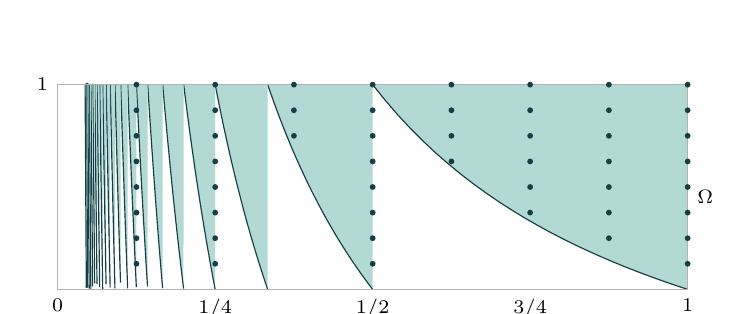
\begin{tikzpicture}[x=8cm,y=2.6cm]
\foreach \m in {1,...,22}{
  \pgfmathsetmacro{\xl}{1/(\m+1)}\pgfmathsetmacro{\xr}{1/\m}
  \fill[sea!44] (\xl,1) -- plot[domain=\xl:\xr,samples=31] (\x,{1/\x-\m}) -- (\xr,1) -- cycle;
  \draw[ink,line width=.42pt] plot[domain=\xl:\xr,samples=26] (\x,{1/\x-\m});
}
\draw[gray!60] (0,0) rectangle (1,1);
\foreach \i in {1,...,8}{\foreach \j in {1,...,8}{
 \pgfmathtruncatemacro{\good}{\j*\i>8*mod(8,\i)}
 \ifnum\good=1\relax\fill[ink] (\i/8,\j/8) circle[radius=1.05pt];\fi}}
\foreach \t/\name in {0/0,0.25/{1/4},0.5/{1/2},0.75/{3/4},1/1}{\node[below,font=\scriptsize] at (\t,0) {$\name$};}
\node[left,font=\scriptsize] at (0,1) {$1$};\node[right,font=\scriptsize] at (1,.45) {$\Omega$};
\end{tikzpicture}\\[-1pt]
{\small The first 22 branches. Dots mark the points of the $8\times8$ grid counted in $\Omega$.}
\end{center}
Write $\gamma_j$ for the Stieltjes constants in the convention $\zeta(1+t)=t^{-1}+\sum_{j\ge0}(-1)^j\gamma_jt^j/j!$. A change of the area measure realizes the entire sequence through the following identities.
\begin{equation}\label{ch4:eq:mell}
 (1+t)\iint_\Omega x^t\,dx\,dy=\zeta(1+t)-1/t,\qquad
 \iint_\Omega\frac{(-\log x)^r}{r!}\,dx\,dy=\sum_{j=0}^r\frac{\gamma_j}{j!}.
\end{equation}
For $t>0$, expand $\lfloor1/x\rfloor=\sum_{m\ge1}\mathbf1_{x\le1/m}$ and integrate. Both sides of the first identity continue analytically to a neighborhood of zero, so comparison of Taylor coefficients proves the second. In particular the first log-weighted area gives $\gamma+\gamma_1$. At the dyadic Hurwitz shift, $\zeta(s,1/2)=(2^s-1)\zeta(s)$ gives
$\gamma_1(1)-\gamma_1(1/2)=2(\log2)\gamma+(\log2)^2$. Both operations retain the same constant. Neither identity supplies an integer numerator for the log-weighted moment. This motivates counting lattice points with the unweighted measure.

\section{Rectangular counts and the surviving area coefficient}\label{ch4:sec:rect}
For integers $a,b\ge1$ let $N(a,b)$ count $(i/a,j/b)\in\Omega$ with $1\le i\le a,1\le j\le b$. Write $D(t)=\sum_{n\le t}\tau(n)$, where $\tau$ counts positive divisors. Direct column counting gives
\[
 N(a,b)=ab+bD(a)-\sum_{i\le a}\lfloor ab/i\rfloor .
\]
Indeed a column contains $b-\lfloor b\{a/i\}\rfloor$ points. Every positive integer pair of product at most $ab$ has first coordinate at most $a$ or second coordinate at most $b$, and all pairs in their $a\times b$ intersection qualify. Therefore
\begin{align}
 C(a,b)&:=N(a,b)+N(b,a)=ab+bD(a)+aD(b)-D(ab),\label{ch4:eq:C}\\
 C(a,b)-2ab\gamma&=b\Delta(a)+a\Delta(b)-\Delta(ab),\label{ch4:eq:delta}
\end{align}
where $\Delta(t)=D(t)-t\log t-(2\gamma-1)t$. In particular $N(n,n)-\gamma n^2=n\Delta(n)-\Delta(n^2)/2$. The elementary bound $\Delta(t)\ll\sqrt t$ follows on splitting $D(t)$ at $\lfloor\sqrt t\rfloor$ and using $H_m=\log m+\gamma+O(1/m)$. It gives $N(n,n)/n^2=\gamma+O(n^{-1/2})$. At $n=8$, $D(8)=20$, $D(64)=280$, giving exactly $N(8,8)=52$.

For real weights $w_{k\ell}$ supported on $1\le k,\ell\le K$ put
\[
 S_w(n)=\sum_{k,\ell}w_{k\ell} C(kn,\ell n),\quad
 r_k=\sum_\ell \ell(w_{k\ell}+w_{\ell k}),\quad b_k=k r_k,\quad
 H=2\sum_{k,\ell}k\ell w_{k\ell}=\sum_k b_k .
\]
Then, exactly,
\begin{equation}\label{ch4:eq:main}
 S_w(n)-H\gamma n^2=n\sum_k r_k\Delta(kn)-\sum_{k,\ell} w_{k\ell}\Delta(k\ell n^2).
\end{equation}
Removing all $r_k$ also removes the area. Conversely any $b$ occurs using only the diagonal weights $w_{kk}=b_k/(2k^2)$. These assertions concern symmetrized rectangles with fixed integer dilations. The second term of \eqref{ch4:eq:main} is $O_w(n)$, smaller than the scale $n^{5/4}$ considered below.

\section{The exact variance of a fixed combination}\label{ch4:sec:variance}
For an arithmetic sequence $b$ supported on $[1,K]$ set $A=b*\tau$, so $A_m=\sum_{k\mid m}b_k\tau(m/k)$. Define $\V_s(b)=\sum_{m\ge1}|A_m|^2/m^s$ for $s>1$. It is finite by the usual divisor bound $\tau(m)\ll_\epsilon m^\epsilon$. Put $E_w(n)=S_w(n)-H\gamma n^2$.
\begin{theorem}\label{ch4:th:variance}
For every fixed real array $w$,
\[
 \lim_{X\to\infty}\frac1X\sum_{n\le X}\frac{E_w(n)^2}{n^{5/2}}
   =\frac{\V_{3/2}(b)}{4\pi^2},\qquad
 \lim_{X\to\infty}X^{-7/2}\sum_{n\le X}E_w(n)^2=\frac{\V_{3/2}(b)}{14\pi^2}.
\]
Both limits are positive if $b\ne0$.
\end{theorem}
\begin{proof}
We use the classical mean-square form of the Vorono\u\i{} approximation, for example Heath-Brown \cite[\S5, eq.~(5.2)]{hb}. In the seminorm $\|f\|_{B^2}^2=\limsup_{X\to\infty}X^{-1}\int_1^X|f(x)|^2\,dx$, $x^{-1/4}\Delta(x)$ is the limit of the trigonometric sums
\[
 \frac1{\pi\sqrt2}\sum_{j\le J}\frac{\tau(j)}{j^{3/4}}\cos(4\pi\sqrt{jx}-\pi/4).
\]
The cited dyadic estimate uses $t=\sqrt x$ and first cuts off the squarefree parts. The change $x=t^2$ preserves convergence in dyadic mean square since its weight is bounded by a constant multiple of its mean there. Each retained squarefree profile converges uniformly in its square-factor index. Distinct frequencies are orthogonal in the limiting mean square and $\sum_j\tau(j)^2j^{-3/2}<\infty$, which also permits the cutoff $j\le J$ above.
For fixed $k$, on $n\le x<n+1$ we have $\Delta(kx)-\Delta(kn)=O_{k,\epsilon}(n^\epsilon+\log(2n))$, by counting the at most $k+1$ jumps. The normalized discrepancy varies by $o(1)$ there, using also $\Delta(kn)\ll_k\sqrt n$. Each finite trigonometric sum varies by $O_{k,J}(n^{-1/2})$. Thus discrete mean squares admit the same approximation. From \eqref{ch4:eq:main}, collecting equal frequencies $m=kj$ gives
\begin{equation}\label{ch4:eq:cos}
 \frac{E_w(n)}{n^{5/4}}\ \sim_{B^2}\
 \frac1{\pi\sqrt2}\sum_{m\ge1}A_m m^{-3/4}\cos(4\pi\sqrt{mn}-\pi/4).
\end{equation}
Here $\sim_{B^2}$ means vanishing seminorm of truncation errors in the limit. For $c\ne0$ the mean of $e^{ic\sqrt n}$ tends to zero. Indeed comparison with its integral on $[1,X]$ costs $O_c(\sqrt X)$ and the integral itself is $O_c(\sqrt X)$. Orthogonality gives the first limit. Partial summation with $n^{5/2}$ gives the factor $2/7$ for the second. At the first nonzero $b_j$, $A_j=b_j$.
\end{proof}
Correlations between rational dilations of $\Delta$ already appear in \cite{amrs}. We now vary all the weights to solve the resulting finite-dimensional optimization.
\section{Optimal weights on every finite divisor-closed set}\label{ch4:sec:opt}
Can signed changes of scale make the variance arbitrarily small while leaving unit area coefficient? For fixed $K$ the answer is quantitative. More generally, let $\mathcal D$ be a nonempty finite set of positive integers that contains every divisor of each of its elements.
\begin{theorem}\label{ch4:th:min}
For real $s>1$ write $D_s=\zeta(s)^4/\zeta(2s)$. Then
\begin{equation}\label{ch4:eq:min}
 \min_{\substack{\operatorname{supp}(b)\subset\mathcal D\\ \sum_k b_k=1}}\V_s(b)
 =\frac{D_s}{\displaystyle\sum_{n\in\mathcal D}
 n^s\prod_{p^2\mid n}(1-p^{-2s})}.
\end{equation}
There is a unique real minimizing vector. Rational vectors of mass one have the same infimum. On $\mathcal D=\{1,\ldots,K\}$ the minimum is asymptotic to
$(s+1)D_s\zeta(2s+2)K^{-(s+1)}$.
\end{theorem}
\begin{proof}
Represent $b$ by $\sum b_k v_k$, where the Gram product of the formal basis is the polarization of $\V_s/D_s$. Explicitly,
\[
 \langle v_k,v_\ell\rangle
 =D_s^{-1}\sum_{m:\,k,\ell\mid m}\tau(m/k)\tau(m/\ell)m^{-s}.
\]
The smallest nonzero component of $b$ survives convolution, so this is positive definite. The series factors by primes. For one prime with $x=p^{-s}$ and local exponents $a,b$, the normalized local factor is
\[
 G_p(a,b)=x^{\max(a,b)}(1+c|a-b|),\qquad c=(1-x)/(1+x).
\]
Indeed the ratio of $\sum_{j\ge0}(j+1)(j+1+|a-b|)x^j$ to $\sum_{j\ge0}(j+1)^2x^j$ is $1+c|a-b|$. The product of the latter sums over all primes is $D_s$. The global Gram product is the product of these normalized local factors.

Denote the prime-coordinate basis by $v_a^{(p)}$, omitting the superscript in the next display. Orthogonalize it by
\[
 u_0=v_0,\quad u_1=v_1-\frac{2x}{1+x}v_0,\qquad
 u_a=v_a-2xv_{a-1}+x^2v_{a-2}\quad(a\ge2).
\]
For $j\le a-2$, $\langle u_a,v_j\rangle=0$ by the second difference of the affine function $1+c(a-j)$. For $j=a-1$ the remaining factor is $(1+c)(1+x)-2=0$. The $a=1$ identity follows directly from $G_p$. The squared norms and coefficient sums $\ell(u_a)$ are
\[
\begin{array}{c|ccc}
 a&0&1&a\ge2\\ \hline
 \|u_a\|^2&1&x(1-x)^2/(1+x)^2& x^a(1-x)^3/(1+x)\\[2pt]
 \ell(u_a)&1&(1-x)/(1+x)&(1-x)^2 .
\end{array}
\]
For $n\in\mathcal D$, multiply the local basis changes over $p^a\Vert n$ (use $u_0$ elsewhere). The resulting vector $U_n$ is $v_n$ plus a combination of its proper-divisor vectors. These $U_n$ therefore form an orthogonal basis of the original space. Their squared norms and their coefficient sums multiply prime by prime. For the functional $L(\sum b_kv_k)=\sum b_k$,
\[
 \|L\|^2=\sum_{n\in\mathcal D}\frac{L(U_n)^2}{\|U_n\|^2}
  =\sum_{n\in\mathcal D}n^s\prod_{p^2\mid n}(1-p^{-2s}).
\]
The minimum squared norm at $L=1$ is $1/\|L\|^2$. Equality occurs at the vector proportional to $\sum_{n\in\mathcal D}L(U_n)U_n/\|U_n\|^2$ with mass one. Undoing the normalization proves \eqref{ch4:eq:min}. Rational mass-one vectors are dense in this real affine space.
Finally $\prod_{p^2\mid n}(1-p^{-2s})=\sum_{d^2\mid n}\mu(d)d^{-2s}$. Its average is $\sum_{d\ge1}\mu(d)d^{-2s-2}=1/\zeta(2s+2)$ by absolute convergence. Partial summation gives the claimed equivalent.
\end{proof}
For a concrete check, at $K=2$ only $1,2$ occur and the denominator of \eqref{ch4:eq:min} is $1+2^s$. At $K=4$ it becomes $1+2^s+3^s+4^s(1-2^{-2s})$.
Specializing to the folded area gives the sharp leading constant
\[
 \inf_{H=1}\lim_{X\to\infty}\frac1X\sum_{n\le X}\frac{|S_w(n)-\gamma n^2|^2}{n^{5/2}}
 \ \sim\ \frac{5\,\zeta(3/2)^4\zeta(5)}{8\pi^2\zeta(3)}\,K^{-5/2}.
\]
The order of the operations matters. This theorem first fixes $K$ and the weights and takes $X\to\infty$. It gives no uniformity in a choice $K=K(X)$. It also optimizes real normalized weights. With raw integer $w$, every $b_k$ is a multiple of $k$, so if $d$ is the first nonzero index then $\V_{3/2}(b)\ge |b_d|^2/d^{3/2}\ge\sqrt d$. Clearing or reducing a denominator is an arithmetic operation with a different cost.

\section{From typical error to rare near-equalities}\label{ch4:sec:law}
A positive mean square does not decide how frequently an error approaches zero. In \eqref{ch4:eq:cos}, write $m=dj^2$ with $d$ squarefree. For independent $U_d$ uniform on $[0,1]$, define
\[
 g_d(u)=\sum_{j\ge1}A_{dj^2}j^{-3/2}\cos(2\pi ju-\pi/4),\qquad
 Y=\frac{1}{\pi\sqrt2}\sum_{d\ {\rm squarefree}}d^{-3/4}g_d(U_d).
\]
The profiles converge uniformly since $|A_m|\ll_b\tau(m)$. The independent centered series converges in $L^2$ by the variance sum in Theorem~\ref{ch4:th:variance}.
\begin{theorem}\label{ch4:th:law}
If $b\ne0$, the sequence $E_w(n)/n^{5/4}$ has the law of $Y$ as its limiting distribution. It has an entire density, positive mass on every nonempty open real interval, and for any sequence $\epsilon_n\downarrow0$,
\[
 \#\{n\le X:|E_w(n)|\le\epsilon_n n^{5/4}\}=o(X).
\]
\end{theorem}
\begin{proof}
The square roots of distinct squarefree positive integers, including $1$, are linearly independent over the rationals. This follows from the square-root monomial basis of the multiquadratic field generated by the finitely many primes involved. Thus for any finite set of such $d$ the vectors $(2\sqrt{dn}\bmod 1)_d$ are uniformly distributed on their torus, by the exponential-sum bound in the proof of Theorem~\ref{ch4:th:variance} and Weyl's criterion. For finite trigonometric polynomials this identifies the limiting laws. The mean-square approximation of \eqref{ch4:eq:cos} and $L^2$ convergence on the random side extend the statement to bounded Lipschitz tests.

Here are details ensuring a density even when the weights have arbitrary signs. Take a squarefree $d$ such that $g_d$ is nonconstant, using the first nonzero $A_m$. If $p>K$ and $p\nmid d$ is prime, every index $k$ from the support dividing $pdj^2$ already divides $dj^2$. For $p\nmid j$, $A_{pdj^2}=2A_{dj^2}$. For all $j$ the two profiles have coefficients bounded in magnitude by $2j^{-3/2}\sum_{k\mid dj^2}|b_k|\tau(dj^2/k)$. This is a summable majorant for fixed $d$. Consequently $g_{pd}\to2g_d$ uniformly as $p\to\infty$. For every fixed real $z\ne0$, $|\E e^{2izg_d(U_d)}|<1$, because a continuous nonconstant function on $[0,1]$ has interval image. The contraction is uniform on compact sets bounded away from zero. For $p$ between $|t|^{4/3}$ and $2|t|^{4/3}$ the magnitude $|t|(pd)^{-3/4}/(\pi\sqrt2)$ belongs to one such compact set. The prime number theorem and independence of the $pd$ components give
\[
 |\E e^{itY}|\le\exp\{-c_b|t|^{4/3}/\log(2+|t|)\}\qquad(|t|\text{ large}).
\]
Fourier inversion converges under every exponential weight, giving an entire density. Its restriction to the real line is nonnegative and integrates to one. Vanishing on an open interval would force it to be identically zero. Finally use a fixed interval $[-\epsilon,\epsilon]$ in the limiting law and then send $\epsilon$ to zero.
\end{proof}
For integer weights and $H\ne0$, infinitely many nonzero $E_w(n)$ tending to zero would prove irrationality. The theorem allows such a subsequence only on a set of density zero. It does prove that every fixed normalized neighborhood of zero occurs with positive density. That neighborhood has width proportional to $n^{5/4}$ in the raw integer count.

\section{Prime intervals for clustered square nodes}
\label{ch4:sec:square-cluster-geometry}

The square-node approximation in VMRC [023] and the signed interpolation in Chapter~\ref{chap:3} motivate a different question. If several nodes are almost equal, how much of their common denominator survives cancellation? A second theorem treats fixed order with no spacing assumption. Write $h(m)=H_{m-1}+1/(2m)$ for positive integers $m$, with $H_0=0$.
For distinct nodes $1\le m_1<\cdots<m_d=M$ and rational weights $c_i$
with $\sum_i c_i=1$, write
\[
 Q=\sum_{i=1}^d c_i\{2h(m_i)-h(m_i^2)\},\qquad
 b=\operatorname{den}(Q),\qquad D=\operatorname{lcm}_i\operatorname{den}(c_i).
\]
Denominators are positive and taken after reduction.
Of particular interest are the barycentric weights of the rational
function
\begin{equation}\label{ch4:cg:sum}
 \frac{u^{d-1}}{\prod_{i=1}^d(u+m_i^2)}
 =\sum_{i=1}^d\frac{c_i}{u+m_i^2},\qquad
 c_i=\frac{(-m_i^2)^{d-1}}{\prod_{j\ne i}(m_j^2-m_i^2)}.
\end{equation}
Expansion at infinity gives $\sum_i c_i=1$.
For these weights $D\mid(2M)!$. Indeed, for $a=m_i$, the product of
the absolute denominator factors is a subproduct of
\[
 \prod_{1\le k\le M,\ k\ne a}|k^2-a^2|
 =\frac{(M-a)!(M+a)!}{2a^2},
\]
which divides $(2M)!$.

\begin{lemma}\label{ch4:cg:prime}
Fix $\delta>0$. For sufficiently large $M$, a prime
$\delta M^2<p<M^2$ with $p\nmid D$ satisfies
\[
                pQ\equiv-\sum_i c_iH_{\lfloor m_i^2/p\rfloor}\pmod p
                \qquad\text{in }\mathbb Z_{(p)}.
\]
A nonzero residue implies $v_p(Q)=-1$.
\end{lemma}
\begin{proof}
Here $p>2M$ and $p^2>M^2$. Multiples of $p$ in $H_{m_i^2-1}$
contribute precisely the stated reciprocals after multiplication by
$p$. Indeed $p\nmid m_i^2$, so replacing $m_i^2-1$ by $m_i^2$ in the
floor does not change it. All the $h(m_i)$ terms and the final
half-corrections are $p$-integral.
\end{proof}

\begin{theorem}[Clustered support]\label{ch4:cg:cluster}
Suppose $M\to\infty$, $m_1/M\to1$ and $\log D=o(M^2)$.
Then, with no restriction on the number of nodes or the signs of
the normalized rational weights,
\[
                          \log b\sim M^2 .
\]
In particular this holds for \eqref{ch4:cg:sum} on every such node sequence.
\end{theorem}
\begin{proof}
Fix an integer $K\ge1$. The intervals
\[
           \left(M^2/(k+1),\ m_1^2/k\right),\qquad 1\le k\le K,
\]
are disjoint and eventually nonempty. For a prime $p$ in the $k$th
interval, $\lfloor m_i^2/p\rfloor=k$ for every $i$.
By Lemma~\ref{ch4:cg:prime}, outside the primes dividing $D$ the residue is
$-H_k$, since the weights sum to one. The fixed positive rationals
$H_1,\ldots,H_K$ exclude only finitely many primes. Discarding primes
dividing $D$ costs at most $\log D$ in logarithmic prime weight.
The prime number theorem, applied to these finitely many endpoints,
therefore yields
\[
 \liminf_{M\to\infty}\frac{\log b}{M^2}
 \ge\sum_{k=1}^K\left(\frac1k-\frac1{k+1}\right)
 =1-\frac1{K+1}.
\]
The integer $2D\operatorname{lcm}(1,\ldots,M^2)$ clears $Q$.
The prime number theorem for the Chebyshev function $\psi$ gives
the matching upper bound as $K\to\infty$.
\end{proof}

\begin{theorem}[Fixed number of moving nodes]\label{ch4:cg:fixed}
For each fixed $d\ge1$ there exist $c_d>0$ and $M_d$ such that the
barycentric weights \eqref{ch4:cg:sum} at \emph{every} choice of $d$
distinct positive integer nodes with $M\ge M_d$ satisfy
\[
                            \log b\ge c_d M^2 .
\]
\end{theorem}
\begin{proof}
If the assertion failed there would be a sequence of configurations
with $M\to\infty$ and $\log b/M^2\to0$. After a subsequence,
all $y_i=m_i^2/M^2$ converge. Group indices by their common limits
and write $0<\lambda_1<\cdots<\lambda_s=1$ for the distinct
positive limits. Write $C_j$ for the sum of the actual weights
in the group with limit $\lambda_j$, and $C_0$ for the sum in a
possible zero group.

We first show $C_0\to0$. On $|z|=\lambda_1/2$ the functions
\[
         \frac{z^{d-1}}{\prod_i(z+y_i)}
                     =\sum_i\frac{c_i}{z+y_i}
\]
converge uniformly to the rational function obtained by replacing
each $y_i$ by its limit. If $d_0$ nodes tend to zero then $d_0\le d-1$.
After cancellation, the limiting function is holomorphic throughout
the closed disk. The integral around its positively oriented boundary,
divided by $2\pi i$, is therefore zero. For large $M$ the corresponding
integral before passage to the limit is exactly $C_0$. This also covers
the case of an empty zero group. In particular
$\sum_{j=1}^s C_j=1+o(1)$.

Put $\lambda_0=0$. For each $1\le j\le s$ choose a nondegenerate
closed interval $I_j$ inside $(\lambda_{j-1},\lambda_j)$ on which
every function $u\mapsto\lfloor\lambda_k/u\rfloor$
($1\le k\le s$) is constant and which contains no point
$\lambda_k/t$, $t$ a positive integer. Such intervals exist because
these threshold sets are locally finite on $(0,1]$.
By uniform separation from all thresholds, for every sufficiently
large configuration and all $u\in I_j$, the harmonic factor
$H_{\lfloor y_i/u\rfloor}$ equals $H_{\lfloor\lambda_k/u\rfloor}$
if $i$ lies in group $k$, and is zero for the zero group. Denote the
common factor by $A_{jk}$. The rational matrix $A=(A_{jk})$ is upper
triangular: it vanishes for $k<j$, and $A_{jj}>0$ since $u<\lambda_j$.
It follows that $Y_j=\sum_{k=1}^s A_{jk}C_k$ is nonzero for at least
one $j$ in each sufficiently late configuration. By a further
subsequence we may fix one such $j$.

There is a fixed common denominator $L$ for the entries of $A$.
The integer $N_M=L(2M)!Y_j$ is nonzero. Formula~\eqref{ch4:cg:sum}
gives $|c_i|\le M^{2(d-1)}$ because the unscaled denominator is a
nonzero integer. It follows that
$\log|N_M|=O_{d,A}(M\log(2M))=o(M^2)$.
Every prime in $M^2I_j$ is $>2M$ for large $M$ and avoids $L(2M)!$.
Outside the primes dividing $N_M$, Lemma~\ref{ch4:cg:prime} now gives
$v_p(Q)=-1$. The prime number theorem places total logarithmic
prime weight $(|I_j|+o(1))M^2$ in this interval; the discarded
primes have weight at most $\log|N_M|$. Thus
$\liminf\log b/M^2\ge |I_j|>0$ on the subsequence, a contradiction.
\end{proof}
\section{Positive kernels, rational weights and denominator growth}\label{ch4:sec:positive}
A large denominator for the square-node family leaves open a different mechanism. A positive integral fixes the sign of the error while signed coefficients cancel its logarithms. The following estimates give separate answers for its real error and its reduced height.
\subsection{Sharp order for arbitrary dyadic support}
Let $h_i=H_i-1/(2i)$, and let $A_i$ denote the Sondow kernel with
polynomial numerator $(xy)^{i-1}(1-x)(1-y)/2$ over
$(1-xy)(-\log(xy))$. For any nonempty finite set $T$ of positive integers
write
$P(z)=\sum_{i\in T}c_i z^{i-1}$, and put
$J(P)$ equal to the integral of $\sum_{i\in T}c_i A_i$ and $S=\sum_{i\in T}i$.
The bivariate numerator is $(1-x)(1-y)P(xy)/2$, so its pointwise
sign is precisely the sign of $P$ on $(0,1)$. Substitution $z=xy$
in the unit square gives
\[
 J(P)=\int_0^1P(z)\omega(z)\,dz,\qquad
 \omega(z)=\frac{1+z}{2(1-z)}+\frac1{\log z}.
\]
Indeed the inner integral of $(1-x)(1-z/x)/(2x)$ from $z$ to $1$
is $[(1+z)(-\log z)-2(1-z)]/2$.
In particular $J(z^{i-1})=\gamma-h_i+\log i$. Indeed the moments of
$\omega+1/2=1/(1-z)+1/\log z$ satisfy
$M_i-M_{i+1}=1/i-\log(1+1/i)$ by Frullani's integral, tend to zero,
and so equal $\gamma-H_{i-1}+\log i$ by the defining limit for
$\gamma$. Thus rational, normalized, logarithm-free polynomials give
actual rational approximations to $\gamma$.

For $0\le z<1$ the weight satisfies
\[
                  (1-z)/12\le\omega(z)\le(1-z)/2 .
\]
To see this, put $u=1-z$ and write
$\omega(1-u)+1/2=[1-\int_0^1(1-u)^sds]/u$.
The binomial series has nonnegative coefficients after the subtraction
and division for $0<s<1$. The constant coefficient is $1/2$, the next
is $1/12$, and the sum of all the remaining coefficients including
that next one is $1/2$, by taking $u\uparrow1$.

\begin{theorem}\label{ch4:st:dyadic-opt}
There exists an absolute constant $C>0$ such that, whenever
$P\ge0$ on $[0,1]$, $P(1)=1$ and $\sum_{i\in T}c_i\log i=0$,
\[
                        J(P)\ge C\frac{\log S}{S^2}
\]
for $S\ge4$. For $D=2^n\to\infty$ the infimum of $J(P)$ under these
conditions over all rational coefficients supported on
$\{1,2,4,\ldots,D\}$ has exact order $(\log D)/D^2$.
The same order holds if real coefficients are admitted.
\end{theorem}
\begin{proof}
On the fixed interval $I=[1/2,1]$, the positive-interval
Newman inequality of Borwein and Erd\'elyi
(\href{https://people.tamu.edu/~terdelyi/papers-online/positive.pdf}
{Theorem~2.1}) gives
$\|P'\|_I\le C_0 S\|P\|_I$. Its hypotheses hold for the increasing
list of the distinct integer exponents $i-1$, adjoining $0$ if absent:
the $j$th exponent is at least $j$ from index zero.
Choose $C_0\ge1$. From a maximizer of $P$ within $I$ there is a
one-sided interval in $I$ of length $1/(4C_0 S)$ on which
$P\ge\|P\|_I/2$. The integral of $1-z$ over any interval of length
$h$ in $[0,1]$ is at least $h^2/2$. Hence $\|P\|_I\ll S^2J(P)$
and $\|P'\|_I\ll S^3J(P)$.

Frullani's identity for each integer $i$ gives
\[
                0=\int_0^1\frac{1-P(z)}{-\log z}\,dz .
\]
Take $a=1-1/S$. Since $-\log z\ge1-z$, the integral of
$P(z)/(-\log z)$ over $[0,a]$ is at most
$12 S^2J(P)$. On $[a,1]$ the absolute value of the integral of
$(P-1)/(-\log z)$ is at most $\|P'\|_I/S$, giving the same order.
On the other hand $\int_0^a dz/(-\log z)\gg\log S$ for $S\ge4$,
as is seen by integrating $1/(2(1-z))$ from $1/2$ to $a$.
This proves the universal bound. For a dyadic support $S<2D$.
A bounded support with $S<4$ gives a fixed positive minimum under the
stated conditions (in fact $P=1$). Monotonicity of $\log S/S^2$ for
$S\ge4$ now gives the lower bound at $D$. For the upper bound let $D=2^n$, $k=D/2$, and choose
$P(z)=n z^{k-1}-(n-1)z^{D-1}$. This polynomial is nonnegative,
$P(1)=1$, and $n\log k=(n-1)\log D$. The weight satisfies
$\omega(z)\sim(1-z)/12$ at $1$, so
$J(z^{i-1})\sim1/(12 i^2)$ by concentration of the beta integral
$\int_0^1z^{i-1}(1-z)\,dz=1/[i(i+1)]$ at $1$.
Consequently $J(P)\sim n/(4D^2)$.
The order statement concerns the actual positive error before clearing
the denominator of the rational approximant; its decay alone does not
prove irrationality.
\end{proof}

\subsection{Reduced denominators for dyadic support}
Write the coefficients of a normalized rational polynomial from
Theorem~\ref{ch4:st:dyadic-opt} as $c_i=a_i/A$, where $a_i\in\mathbb Z$,
$A=\sum_i a_i>0$, and $\gcd_i a_i=1$. Let $D=2^n$ be its largest
occupied index, let $r=\sum_i c_i h_i$, and put $E=\gamma-r=J(P)>0$.
Write $\vartheta(x)=\sum_{p\le x}\log p$, summing over primes.
\begin{proposition}\label{ch4:st:dyadic-height}
Uniformly over all such polynomials with $D\ge4$,
\[
 \log\big(\operatorname{den}(r)E\big)
 \ge \vartheta(D)-\vartheta(D/2)-\log A-O((\log D)^3).
\]
Consequently, if $D\to\infty$ and $\log A=o(D)$, the lower limit of
$D^{-1}\log(\operatorname{den}(r)E)$ is at least $1/2$.
If in addition $E\le1$, this lower bound improves to $\log 2$.
\end{proposition}
\begin{proof}
Let $m$ be the number of occupied indices. For $0\le j<m$, the
moments $\int_0^1z^j(1-z) A P(z)\,dz$ have absolute value at most
$12AE$ by positivity and the weight bound. Their matrix in the
coefficients $a_i$ has entries $1/[(i+j)(i+j+1)]$. The matrix is
nonsingular. Indeed a nonzero linear combination of the $m$ monomials
has at most $m-1$ positive zeros by Descartes' rule. Multiplication by
the polynomial whose simple roots are its sign changes on $(0,1)$
produces a nonzero polynomial of constant sign, contradicting
orthogonality to all degrees below $m$ against $1-z$. Every entry
denominator is at most $(2D)^2$. Their product clears the determinant,
whose absolute value is thus at least $(2D)^{-2m^2}$. The absolute
cofactors are at most $m!$ by the determinant expansion. Since
$m\le1+\log_2 D$, inversion gives, uniformly,
\[
                     \max_i|a_i|\le AE\exp(O((\log D)^3)).
\]
For every prime $D/2<p<D$, all $h_i$ with $i<D$ are $p$-integral
and $p h_D\equiv1\pmod p$. If $p\nmid a_D$, it follows that
$v_p(Ar)=-1$, hence $v_p(r)=-1-v_p(A)\le-1$, including when $p\mid A$.
The total logarithmic weight of excluded primes is at most $\log|a_D|$.
The uniform bound follows, and then the prime number theorem gives $1/2$.

For the refinement, write $a_{D/2^j}=0$ at absent indices and fix an
integer $H\ge3$. In each interval $D/(h+1)<p<D/h$, $1\le h\le H$,
reduction of $pAr$ modulo $p$ gives the rational residue
\[
                  V_h=\sum_{j:\,2^j\le h}a_{D/2^j}H_{\lfloor h/2^j\rfloor}.
\]
This holds for all large $D$, since $p^2>D$, $p$ is odd, and each $i$
is a power of two. Each nonzero $V_h$ has numerator of magnitude
$\ll_H\max_i |a_i|=\exp(o(D))$ under $E\le1$, $\log A=o(D)$.
Thus each such interval contributes its full limiting weight
$1/[h(h+1)]$ to $D^{-1}\log\operatorname{den}(r)$, up to $o_H(1)$,
uniformly even when the nonzero intervals vary with $D$.
Now $V_1=a_D\ne0$, and $V_{2j+1}-V_{2j}=a_D/(2j+1)\ne0$.
In each pair of intervals indexed by $2j,2j+1$ at least the weight
of the shorter interval survives. Taking the lower limit and then
$H\to\infty$ gives $\sum_{j\ge0}1/[(2j+1)(2j+2)]=\log2$.
Theorem~\ref{ch4:st:dyadic-opt} gives $\log E\ge-O(\log D)$, proving the
same lower bound for the product.
\end{proof}
Thus a successful sequence of rational dyadic centers must pay a specific price in its coefficients. If $\operatorname{den}(r)(\gamma-r)\to0$, Theorem~\ref{ch4:st:dyadic-opt} forces $D\to\infty$, and Proposition~\ref{ch4:st:dyadic-height} gives
\[
 \liminf\frac{\log A}{D}\ge\frac12 .
\]
Allowing arbitrary primitive coefficient sums changes the question again.
\begin{corollary}[Three-atom realizability]\label{ch4:st:three-dyadic}
Every rational number $r$ with $1/2\le r<\gamma$ is the exact center
$\sum_i c_i h_i$ of a polynomial $P$ with rational coefficients that
satisfies $P(1)=1$, $P>0$ on $(0,1)$, and $\sum_i c_i\log i=0$.
Its support lies in $\{1,2^{n-1},2^n\}$ for some $n\ge2$.
In this three-atom class, the existence of a sequence of centers
$r_j=a_j/b_j$ in lowest terms with $b_j(\gamma-r_j)\to0$ is
equivalent to the irrationality of $\gamma$.
\end{corollary}
\begin{proof}
The constant polynomial $1$ has center $h_1=1/2$, and $\gamma>1/2$
since $J(1)>0$. Write $U_n(z)=nz^{2^{n-1}-1}-(n-1)z^{2^n-1}$.
Its rational centers $r_n$ approach $\gamma$ strictly from below by
the preceding estimates. For $1/2<r<\gamma$, take $r_n>r$ and set
$t=(r-1/2)/(r_n-1/2)$. The polynomial $(1-t)+tU_n$ has all the
stated properties. If $\gamma$ is irrational, its lower continued
fraction convergents eventually belong to this interval and satisfy
$b_j(\gamma-r_j)<1/b_j$. Conversely, for $\gamma=u/v$ in lowest
terms, each positive value of $b_j(\gamma-r_j)$ is at least $1/v$.
\end{proof}
\section{Carry words at the Dirichlet hyperbola}\label{ch4:sec:carry}
A large primitive error motivates changing the observation itself. We record the individual changes of a floor function in neighboring columns.
For integers $1\le m\le n$ and $j\ge1$, put
\[
 c_j(n,m)=\left\lfloor\frac{n^2+jn}{m}\right\rfloor
 -\left\lfloor\frac{n^2+(j-1)n}{m}\right\rfloor
 -\left\lfloor\frac nm\right\rfloor\in\{0,1\}.
\]
These carries count changes in lattice-point columns. Writing
$D(x)=\sum_{ab\le x}1$ for positive integer pairs $(a,b)$, the hyperbola
identity $D(x)=2\sum_{m\le\sqrt x}\lfloor x/m\rfloor-\lfloor\sqrt x\rfloor^2$
gives the exact relation
\[
 2\sum_{m\le n}c_1(n,m)=D(n^2+n)-D(n^2)-2D(n).
\]
The classical one-variable mean $n^{-1}\sum_{m\le n}\{n/m\}\to1-\gamma$
goes back to de la Vall\'ee Poussin. See F.~Pillichshammer, \emph{Euler's
constant and averages of fractional parts}, Theorem~0 in \cite{pill}. To distinguish the
individual carry words we also need the initial intercept $\{n^2/m\}$.

\paragraph{Word law.}
For $w\in\{0,1\}^r$, let $P_n(w)$ be the proportion of $m\le n$ having
$(c_1,\ldots,c_r)=w$. Write $s_0=0$, $s_j=\sum_{i=1}^j w_i$, and
$[z]_+=\max(z,0)$. With $\psi=\Gamma'/\Gamma$ we have
\begin{align*}
 P(w):=\lim_{n\to\infty}P_n(w)
 &=\int_0^1 \ell_w(t)\psi'(1+t)\,dt,\\
 \ell_w(t)&=\big[1+\min_{0\le j\le r}(s_j-jt)
                     -\max_{0\le j\le r}(s_j-jt)\big]_+ .
\end{align*}
To prove the formula, set $x=m/n$, $t=\{1/x\}$, $y=\{n^2/m\}$.
Telescoping gives $\sum_{i=1}^j c_i=\lfloor y+jt\rfloor$. The conditions
$\lfloor y+jt\rfloor=s_j$ cut out an interval of length $\ell_w(t)$ in
$0\le y<1$. Fix $0<\varepsilon<1$. On each fixed subinterval of
$[\varepsilon n,n]$, the second derivative of $h n^2/u$ has magnitude
$\asymp_{h,\varepsilon} n^{-1}$ for every nonzero integer $h$. The van der
Corput second-derivative estimate consequently bounds the exponential sum
there by $O_{h,\varepsilon}(\sqrt n)$. By Weyl's criterion on each such
subinterval, rectangle counts for $(m/n,\{n^2/m\})$, normalized by $n$,
converge to rectangle areas in $[\varepsilon,1]\times[0,1]$. The word test
is Riemann integrable there because its discontinuities lie on finitely many
piecewise smooth curves. Passing to the limit and then letting
$\varepsilon\downarrow0$ gives $\int_0^1\ell_w(\{1/x\})\,dx$.
The substitution $x=(k+t)^{-1}$ on each branch supplies the density
$\sum_{k\ge1}(k+t)^{-2}=\psi'(1+t)$.

\paragraph{One and two carries.}
For constant words the interval lengths are $[1-rt]_+$ and
$[1-r(1-t)]_+$. Integration by parts, with $\psi(1)=-\gamma$ and
$\psi(2)=1-\gamma$, gives
\[
 P(0^r)=\gamma+r\log\Gamma(1+1/r),\qquad
 P(1^r)=1-\gamma+r\log\Gamma(2-1/r).
\]
In particular $P(0)=\gamma$, $P(1)=1-\gamma$. Since the intercept is
uniform conditionally on $t$, its translate by $t$ modulo one has the
same law. The one-letter marginals at the two positions therefore agree,
and $\Gamma(3/2)=\sqrt\pi/2$ gives
\begin{align*}
 P(00)&=\gamma+\log(\pi/4), & P(11)&=1-\gamma+\log(\pi/4),\\
 P(01)&=\log(4/\pi), & P(10)&=\log(4/\pi).
\end{align*}

\paragraph{Threshold counts and cyclotomic units.}
For $0\le a\le q$ integral, the following geometric statistic depends
only on the rational number $u=a/q$. Its value is
\[
 Y(u)=\lim_{n\to\infty}\frac1{nq}\sum_{m=1}^n
 \bigg[\sum_{j=1}^q c_j(n,m)-a\bigg]_+
 =(1-u)(1-\gamma)+\log\Gamma(1+u).
\]
Indeed, for fixed $t$, $\lfloor y+qt\rfloor$ takes the two neighboring
integer values of $qt$ with mean $qt$ under uniform $y$. The function
$[z-a]_+$ is affine between adjacent integers. Integrating first in $y$
then gives $Y(u)=\int_u^1(t-u)\psi'(1+t)\,dt$, which yields the displayed
identity by integration by parts.

For primes $p\ge5$ and $2\le a\le(p-1)/2$, set
\[
 U_{p,a}=Y(a/p)+Y(1-a/p)-Y(1/p)-Y(1-1/p).
\]
The numbers $1$ and all $U_{p,a}$ are linearly independent over
$\overline{\mathbb Q}$. To prove this, the reflection formula gives
\[
 \exp U_{p,a}=\frac{a(p-a)}{p-1}\,
                 \frac{\sin(\pi/p)}{\sin(\pi a/p)}.
\]
The positive numbers $v_{p,a}=\sin(\pi a/p)/\sin(\pi/p)$ are algebraic
units. In fact they differ by roots of unity from
$(1-\zeta_p^a)/(1-\zeta_p)$, where $\zeta_p=e^{2\pi i/p}$; the quotient
and its reciprocal are algebraic integers by finite geometric sums.
The cyclotomic-unit independence theorem across distinct prime conductors
makes the family $v_{p,a}$ multiplicatively independent. To pass from
the complex quotients in that theorem to their positive absolute values,
raise any putative relation to a common multiple of the orders of the
roots of unity involved. See T.~Chatterjee and S.~Dhillon,
\emph{Canad. Math. Bull.} \textbf{63} (2020), 31--45, Proposition~2.3,
DOI 10.4153/S0008439519000468. A multiplicative relation among the
$\exp U_{p,a}$ would make the corresponding product of $v_{p,a}$ a
positive rational algebraic unit, necessarily $1$. Their independence
forces every exponent to vanish. Baker's theorem now gives the assertion
with $1$ included (ibid., Proposition~2.1).

Each $Y(a/q)$ is a rational linear combination of length-$q$ word
probabilities, and $1$ is their sum. Thus the $\overline{\mathbb Q}$-span
of the probabilities of words of lengths at most $R$ has dimension at least
\[
 1+\sum_{\substack{5\le p\le R\\p\ {\rm prime}}}\frac{p-3}{2}
 \sim\frac{R^2}{4\log R},
\]
by partial summation and the prime number theorem. Here the difference
defining $U_{p,a}$ cancels the term involving $\gamma$. The rank bound
therefore supplies no arithmetic classification of the one-letter
probability $P(0)=\gamma$.
\subsection{The full span and its quadratic growth}
Let $\mathcal F_R$ be the rational numbers in $[0,1]$ of reduced
denominator at most $R$. Let $V_R$ be the rational span of all $P(w)$
for $1\le |w|\le R$. Then
\[
 V_R=\operatorname{span}_{\mathbb Q}
 \bigl(\{1,\gamma\}\cup
 \{\log\Gamma(1+u):u\in\mathcal F_R\cap(0,1)\}\bigr).
\]
In fact every $\ell_w$ is continuous piecewise affine with integer slopes
and knots in $\mathcal F_R$. A change of minimizing or maximizing index
requires equality of two affine functions $s_j-jt$. Truncation at zero
adds only solutions of $1+s_j-jt=s_k-kt$. In either case a nonconstant
equation has denominator at most $|w|$. Each $\ell_w$ is therefore a
rational linear combination of $1,t$ and $[t-u]_+$ for interior Farey
knots $u$, obtained by adding successive slope changes. Their integrals
against the word-law density are $1,Y(0),Y(u)$. Conversely each $Y(a/q)$
is a rational linear combination of length-$q$ word probabilities, $1$
is their sum, and $\gamma=1-Y(0)$. The threshold formula proves the
equality.

Write $d_R=\dim_{\overline{\mathbb Q}}\operatorname{span}_{\overline{\mathbb Q}} V_R$.
We have
\[
 \frac{9}{\pi^4}\le\liminf_{R\to\infty}\frac{d_R}{R^2}
 \le\limsup_{R\to\infty}\frac{d_R}{R^2}\le\frac{3}{\pi^2}.
\]
The upper bound follows from $d_R\le |\mathcal F_R|
=1+\sum_{q\le R}\varphi(q)$. For the lower bound extend the definition of
$U_{p,a}$ to $U_{q,a}$ using all $3\le q\le R$ and all $1\le a<q$
coprime to $q$. Reflection gives the same positive algebraic
$\exp U_{q,a}$ with $q$ in place of $p$.

Let $L=\operatorname{lcm}(1,\ldots,R)$, $K=\mathbb Q(\zeta_L)$,
$G=\operatorname{Gal}(K/\mathbb Q)$, and use additive notation $[z]$
for the image of $z$ in $(K^\times/\mathbb Q^\times)\otimes_{\mathbb Z}\mathbb C$.
Put $\beta_{q,a}=(1-\zeta_q^a)(1-\zeta_q^{-a})$ and let $W$ be the complex
span of $[\beta_{q,a}/\beta_{q,1}]$. As $[\exp(2U_{q,a})]
=-[\beta_{q,a}/\beta_{q,1}]$, the multiplicative rank of the positive
$\exp(2U_{q,a})$ is at least $\dim W$. Here $\exp(2U_{q,a})$ lies in $K$
even when a sine itself requires a larger field. For $b\in G$ acting
by $\zeta_L\mapsto\zeta_L^b$, one has
$\sigma_b[\beta_{q,a}/\beta_{q,1}]=[\beta_{q,ba}/\beta_{q,b}]$, so $W$
is stable under $G$.

Each primitive even nonprincipal character $\chi$ of conductor $q\le R$
gives a vector
\[
 X_\chi=\sum_{a\in(\mathbb Z/q\mathbb Z)^\times}\overline{\chi(a)}
              [\beta_{q,a}/\beta_{q,1}]\in W.
\]
Its coefficients sum to zero, so changing $a$ to $ba$ gives
$\sigma_b X_\chi=\chi(b)X_\chi$. The additive functional on $K^\times$
\[
 z\longmapsto\log|z|-\frac{1}{|G|}\sum_{\sigma\in G}\log|\sigma z|
\]
vanishes on $\mathbb Q^\times$ and extends complex linearly to our
ambient space. The Galois average is the same for all the conjugates
$\beta_{q,a}$. Thus this functional sends $X_\chi$ to
\[
 2\sum_{a\in(\mathbb Z/q\mathbb Z)^\times}\overline{\chi(a)}
       \log(2\sin(\pi a/q))
   =-2\tau(\overline\chi)L(1,\chi)\ne0.
\]
Here $a$ ranges over representatives $1\le a<q$.
The identity follows from the primitive Gauss sum and the Fourier
series of $\log(2\sin\pi t)$; see N.~Elkies, \emph{Formulas for
$L(1,\chi)$}, Harvard Math~259, equation~(2).
The nonvanishing follows from $|\tau(\overline\chi)|=\sqrt q$ and
Dirichlet's nonvanishing theorem. Distinct primitive characters inflate
to distinct characters of $G$ by uniqueness of the primitive conductor.
Their nonzero eigenvectors are independent. Selecting a multiplicatively
independent subset of the positive $\exp(2U_{q,a})$ and applying Baker's
theorem gives $d_R\ge E(R)$, where $E(R)$ counts the primitive even
nonprincipal characters of conductor at most $R$.

For completeness, the number of all primitive characters of conductor
$q$ is $(\mu*\varphi)(q)$, by uniqueness of induction and M\"obius
inversion. From $\sum_{n\le x}\varphi(n)=x^2/(2\zeta(2))+O(x\log(2x))$,
another summation yields
\[
 \sum_{q\le R}(\mu*\varphi)(q)
  =\frac{R^2}{2\zeta(2)^2}+O(R\log^2(2R)).
\]
The even-minus-odd count among all characters modulo $q$ is
$\sum_{\chi\bmod q}\chi(-1)$, which equals $1$ for $q=1,2$ and is zero
otherwise. M\"obius inversion shows that the corresponding primitive
difference is $\mu(q)+\mathbf 1_{2\mid q}\mu(q/2)$, with the second term
interpreted as zero for odd $q$. Its sum is $O(R)$. Dividing by two and
discarding the principal character gives
$E(R)=9R^2/\pi^4+O(R\log^2(2R))$, as claimed.

The reflected statistics themselves have a sharper rank asymptotic.
All $\beta_{q,a}/\beta_{q,1}$ are units, by the geometric-sum argument.
Units inject into $K^\times/\mathbb Q^\times$ up to the finite group
$\{1,-1\}$. Dirichlet's unit theorem identifies their complexified
logarithmic embedding with the augmentation-zero subspace of
$\mathbb C[G/\{1,-1\}]$ (the coordinates are the conjugate pairs of
embeddings). Each nonprincipal even character consequently has multiplicity
one and every other character has multiplicity zero. Each generator at
$q$ is fixed by the kernel of $G\to(\mathbb Z/q\mathbb Z)^\times$, so its
character components have conductor dividing $q$. This proves
$\dim W=E(R)$. In passing from the units to the positive $\exp(2U_{q,a})$,
all rational factors are supported on primes at most $R$. The kernel
of their multiplicative span's projection to $K^\times/\mathbb Q^\times$
therefore has rank at most $\pi(R)$, where $\pi(R)$ counts these primes.
Indeed any rational product in this span is a rational factor so supported
times an algebraic unit, which must then be a rational unit. By Baker's
theorem, the $\overline{\mathbb Q}$-rank of the family of $U_{q,a}$ itself
is $E(R)+O(\pi(R))\sim9R^2/\pi^4$.
\section{A two-frequency test using only integer grid counts}\label{ch4:sec:test}
The limiting law of Section~\ref{ch4:sec:law} probes a fixed frequency of the normalized discrepancy. Original rationality concerns lattice spacings of one in the raw count. To retain that spacing, use a second resolution, independent of the index in the exponential sum. Let $X$ be a positive integer, $M=X^5$, $R_X=N(M,M)/M^2$ and $e(z)=\exp(2\pi iz)$. Define the real algebraic number
\[
 T_X=\sum_{h=1}^{2}\left|\frac1X\sum_{n=1}^X e(hn^2 R_X)\right|^2.
\]
All input consists of finite integer counts. For example, $N(M,M)$ can be computed from \eqref{ch4:eq:C} with integer division alone.
\begin{theorem}\label{ch4:th:test}
The limit of $T_X$ exists. It is zero exactly when $\gamma$ is irrational. If $\gamma=a/b$ in lowest terms with $b>0$, the limit equals
\[
 \begin{cases}
  6/b,&8\mid b,\\
  2/b,&8\nmid b.
 \end{cases}
\]
\end{theorem}
\begin{proof}
The square-grid estimate gives $R_X-\gamma=O(X^{-5/2})$. Since $n\le X$ and $h\le2$, replacing $R_X$ by $\gamma$ in either average costs $O(X^{-1/2})$. If $\gamma$ is irrational, Weyl's theorem on a quadratic polynomial with irrational leading coefficient gives zero for both limiting averages. Equivalently, finite differencing with step $j\ne0$ reduces the mean square to geometric progressions with ratio $e(2hj\gamma)\ne1$, followed by a limit in the number of steps.

If $\gamma=a/b$, the limiting average at frequency $h$ is the complete quadratic sum $G(v,q)/q$, with $q=b/\gcd(b,h)$ and $v/q=ha/b$ in lowest terms. To compute its norm square, set one summation variable equal to the other plus $j$. Orthogonality gives
\[
 |G(v,q)|^2=q\!\!\sum_{j\bmod q:\,q\mid2j}e(vj^2/q)
 =\begin{cases}q,&q\ {\rm odd},\\0,&q\equiv2\pmod4,\\2q,&4\mid q.\end{cases}
\]
The formula includes $q=1$. Applying it first with $q=b$ and then with $q=b/\gcd(b,2)$ proves the assertion. A single frequency $h=1$ misses denominators congruent to $2$ modulo $4$.
\end{proof}
For comparison, Sondow's integral criteria already give equivalences for the same named question \cite{sondow}. The two-frequency computation gives an exact target for the lattice construction. Its proof determines the alternatives but supplies no upper bound $T_X=o(1)$. Fixed-frequency convergence of the normalized discrepancies cannot be used at the growing frequencies required after multiplying them by $n^{5/4}$.

\section{Ten attempts and the status of the original question}\label{ch4:sec:audit}
The common target in every round is $\gamma\notin\mathbb Q$. G1 (the pre-existing problem), G2 (the original number and proposition) and G3 (its documented open status) apply throughout. The table records both the mathematical gain and the step that prevented G4 (a complete proof). For G5 the estimates below have content beyond rewriting an identity, but none is sufficient to resolve the named problem. G6, historical priority for a solution, is unestablished.
\par\medskip\begin{small}
\renewcommand{\arraystretch}{1.19}
\noindent\begin{tabular}{@{}l>{\raggedright\arraybackslash}p{.39\linewidth}>{\raggedright\arraybackslash}p{.48\linewidth}@{}}
\toprule
No. & Question and outcome & Remaining obstruction or consequence\\\midrule
1 & Test the slope by integer points. & A nonzero error approaching zero would suffice. The line alone gives no such construction.\\
2 & Fold the hyperbola and take log-weighted areas. & The area is $\gamma$ and the next moment is $\gamma+\gamma_1$. The log-weighted moment has no proved integer discretization at unit accuracy.\\
3 & Count the area on rectangular grids. & Symmetrization gives the exact divisor-error identity \eqref{ch4:eq:delta}.\\
4 & Vary the aspect ratios to remove the error. & Complete leading cancellation forces $H=0$. The same operation erases the target area.\\
5 & Minimize the surviving mean square. & Theorem~\ref{ch4:th:min} gives the exact optimum at every fixed cutoff. Adaptive cutoffs require uniform estimates and arithmetic control.\\
6 & Search the rare indices hidden by a mean square. & Every fixed normalized interval has positive mass. Indices reaching a shrinking normalized interval have density zero, yet may be infinite.\\
7 & Return to the signed square-node estimates. & Prime intervals detect exponential reduced denominators even at clustered nodes. Separated scales at growing order remain outside the two height theorems.\\
8 & Permit positive kernels with many signed dyadic coefficients. & Small coefficient sums force exponential integerized error. Three unrestricted atoms can represent every rational from $1/2$ up to $\gamma$. Selecting successful centers is exactly the missing arithmetic.\\
9 & Resolve individual carry words, then compare all lengths. & Their span has quadratic growth. Reflection proves independence in directions that cancel $\gamma$.\\
10 & Test at unit spacing using a finer grid. & Two fixed quadratic frequencies detect every rational denominator. An unconditional bound $T_X=o(1)$ is still missing.\\
\bottomrule
\end{tabular}\par
\end{small}

\paragraph{Sources and scope of the comparison.}
The corpus snapshot is \cite{corpus}. For the target we consulted the sections on Stieltjes transfers, prime support and positive moments in [019], the shear computations in [020], the local arithmetic of linear forms in [021], and the square-node construction in [023]. The comparisons of positive kernels and reduced denominators also use [033], [098], [105] and the Stieltjes recovery discussion in [170]. Section~\ref{ch3:sq:section} treated a separated largest square node. Section~\ref{ch4:sec:square-cluster-geometry} supplies estimates for clustered supports and arbitrary configurations of a fixed number of barycentric nodes. These different hypotheses are stated explicitly. The class of positive dyadic polynomials in Section~\ref{ch4:sec:positive} imposes additional positivity and exact-log constraints.

The area identity, the divisor-error expansion, the one-error distribution and the covariance of rational dilations have classical or published sources \cite{lagarias,pill,hb,amrs}. The extremum \eqref{ch4:eq:min} solves a further finite optimization using orthogonalization. Diagonalization of multiplicative quadratic forms is also classical in sieve theory, for example in \href{https://kskedlaya.org/ant/chap-selberg.html}{the Selberg sieve}. The word calculation uses the classical theory of cyclotomic units and linear forms in logarithms \cite{cd}. The lower and upper dimension bounds do not establish the independence of the Stieltjes constants or of arbitrary log-gamma values. The bibliographic comparison establishes no historical priority for the deductions in this note.

% ===== Source 5: Euler_Gamma_Lattice_Resolution.tex =====
\chapter[Lattice counts and resolution]{Which lattice counts can detect the irrationality of Euler's constant?}\label{chap:5}
{\noindent\large\itshape A resolution threshold and the arithmetic cost of signed weights\par}\vspace{9pt}
\noindent\textbf{Abstract.}\enspace We transfer a counting argument for jumps of fractional parts to the original Euler--Mascheroni constant. A circle divided into three arcs gives a rational statistic on integer lattice counts. Its limiting variance at every rational slope is computed explicitly and is at least the reciprocal of nine times the reduced denominator. When a square grid of side $M$ measures the folded-hyperbola area and the quadratic orbit has length $\lfloor M^u\rfloor$, the behavior changes at $u=3/8$. Above this threshold the unmodified statistic tends to zero in density under both arithmetic alternatives. At the threshold its mean still distinguishes the alternatives. Separately, an integer lattice of coefficients gives the sharp order of the least normalization needed to realize each fixed rational center in a family of positive dyadic approximants. These results locate a loss of arithmetic information and quantify a cost previously bounded on only one side. They leave the irrationality of Euler's constant open.

\section{The input from the corpus and the original slope}
Write $e(t)=\exp(2\pi i t)$, $\|t\|=\min_{k\in\mathbb Z}|t-k|$ and
$\gamma=\lim_{m\to\infty}(H_m-\log m)$ with $H_m=\sum_{j=1}^m1/j$. The question is whether $\gamma\in\mathbb Q$ \cite{lagarias,brent,sondow}. In VMRC [200], the lemma on weighted fractional-part descent uses the following exact balance for $F(s)=\sum_j c_j\{t_j+r_js\}$ with $c_j>0$, $r_j$ positive integers, and $C=\sum r_jc_j$. If a jump at $v$ has total size $J_v$, then
\[
 \frac1C\sum_v J_vF(v)=\frac12\sum_j c_j-\frac1{2C}\sum_v J_v^2.
\]
This follows by integrating the smooth derivative of $F^2$ and adding its jumps around one period. The term $\sum J_v^2$ counts coincident events with multiplicity. Our phases approximate an unknown slope, so exact coincidence is unstable. We instead group crossings in a rotating interval and integrate the square of their count. This preserves near coincidences at a specified angular scale. VMRC [224] also compares collisions and angular averages under different arithmetic hypotheses. VMRC [045] tracks the index of an integral coefficient lattice. Section~\ref{ch5:dl:sec} calculates such an index for our dyadic approximants. All corpus references use snapshot \cite{corpus}.

The region and grid from Chapter~\ref{chap:4} are
\[
 \begin{gathered}
 \Omega=\{(x,y)\in(0,1]^2:\{1/x\}<y\},\qquad R_M=N(M,M)/M^2,\\
 N(a,b)=\#\{1\le i\le a,\ 1\le j\le b:(i/a,j/b)\in\Omega\}.
 \end{gathered}
\]
On $1/(k+1)<x<1/k$ its area is $1/k-\log(1+1/k)$, so the full area is $\gamma$. Define $D(t)=\sum_{j\le t}\tau(j)$, where $\tau$ counts divisors, and $\Delta(t)=D(t)-t\log t-(2\gamma-1)t$. Counting the columns and interchanging coordinates gives
\begin{align}
 N(a,b)&=ab+bD(a)-\sum_{i\le a}\lfloor ab/i\rfloor,\label{ch5:neq}\\
 N(M,M)&=\tfrac12\{M^2+2MD(M)-D(M^2)\},\nonumber\\
 Y_M:=M^{3/4}(R_M-\gamma)&=M^{-1/4}\Delta(M)-\tfrac12M^{-5/4}\Delta(M^2).\label{ch5:yeq}
\end{align}
The hyperbola method gives $\Delta(x)=O(\sqrt x)$ and the last term of \eqref{ch5:yeq} tends to zero. In particular $R_M\to\gamma$. The original two-frequency test used $M=X^5$ and the absolute squares of $X^{-1}\sum_{n\le X}e(hn^2R_M)$ for $h=1,2$. Our first question is how much of that resolution the unmodified square grid actually needs.

\section{One rotating interval and an exact denominator formula}\label{ch5:sec:sector}
For $\alpha\in\mathbb R$, $x_n=\{n^2\alpha\}$, and $s\in\T$ let $B_X(s)$ be the proportion of $1\le n\le X$ with $x_n\in[s,s+1/3)$ modulo one. Define $V_X(\alpha)=\int_0^1(B_X(s)-1/3)^2ds$. If $(y)_+=\max(y,0)$, the overlap of two arcs gives the exact formula
\begin{equation}\label{ch5:vsum}
 V_X(\alpha)=\frac1{X^2}\sum_{i,j\le X}\left(\tfrac13-\|(i^2-j^2)\alpha\|\right)_+-\tfrac19 .
\end{equation}
In particular the output is rational for every rational grid estimate. The same information can be recovered through the frequencies of the square orbit. Put $S_X(h;\alpha)=X^{-1}\sum_{n\le X}e(hn^2\alpha)$. Parseval gives the absolutely convergent series
\begin{equation}\label{ch5:four}
 V_X(\alpha)=\sum_{h\ne0}c_h|S_X(h;\alpha)|^2,\qquad
 c_h=\frac{\sin^2(\pi h/3)}{\pi^2h^2},\qquad \sum_{h\ne0}c_h=2/9 .
\end{equation}
The two nonzero coefficients at $h=1,2$ will be important.
\begin{center}
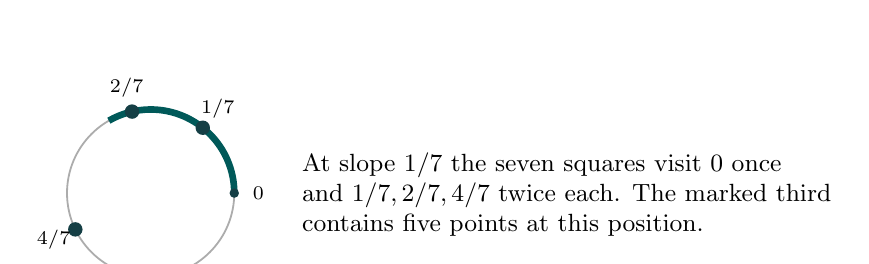
\begin{tikzpicture}[scale=.90]
\draw[gray!65,line width=.65pt] (0,0) circle (1.18);
\draw[teal!70!black,line width=2.4pt] (1.18,0) arc[start angle=0,end angle=120,radius=1.18];
\foreach \i/\lab in {0/{0},1/{1/7},2/{2/7},4/{4/7}}{
 \ifnum\i=0 \def\sz{1.9pt}\else\def\sz{2.9pt}\fi
 \fill[ink] ({360*\i/7}:1.18) circle (\sz);
 \node[font=\scriptsize] at ({360*\i/7}:1.52) {$\lab$};}
\node[align=left,anchor=west,font=\small] at (2,-.02) {At slope $1/7$ the seven squares visit $0$ once\\
and $1/7,2/7,4/7$ twice each. The marked third\\contains five points at this position.};
\end{tikzpicture}
\end{center}

\begin{theorem}\label{ch5:th:q}
For a reduced rational $\alpha=a/b$, write $b=2^\nu3^\kappa m$ with $(m,6)=1$. Then
\begin{equation}\label{ch5:vform}
 V_3(b):=\lim_{X\to\infty}V_X(a/b)
 =\frac{2\,3^\kappa F_2(\nu)}{9b^2}
   \prod_{p^\ell\Vert m}\left(p^\ell+p^{\ell-1}-p^{-1}\right)
 \ \ge\ \frac1{9b},
\end{equation}
where $F_2(0)=1$ and $F_2(\nu)=3\cdot2^\nu-5$ for $\nu\ge1$. When $b\mid X$ the finite statistic already equals this limit. If $\alpha_X\to\alpha$ with $\alpha$ irrational, $V_X(\alpha_X)\to0$ with no rate hypothesis on $\alpha_X-\alpha$.
\end{theorem}
\begin{proof}
For reduced $v/q$, subtraction of the two summation indices in the squared complete quadratic sum gives
\[
 w(q):=\left|\frac1q\sum_{j\bmod q}e(vj^2/q)\right|^2
 =q^{-1}\!\!\sum_{j\bmod q:\ q\mid2j}e(vj^2/q)
 =\frac{\lambda(q)}q,\qquad
 \lambda(q)=
 \begin{cases}1&q\ {\rm odd},\\0&q\equiv2\pmod4,\\2&4\mid q.\end{cases}
\]
At frequency $h$ put $q=b/\gcd(b,h)$. The limit in \eqref{ch5:four} is $\sum_{h\ne0}c_hw(b/\gcd(b,h))$. The weights on positive $h$ are $3/(4\pi^2h^2)$ if $3\nmid h$ and zero otherwise. Group $h=(b/q)j$ with $(j,q)=1$. Summing over $j$ by its Euler product gives
\[
 V_3(b)=\frac1{4b^2}
 \sum_{\substack{q\mid b\\3\nmid b/q}} q\,\lambda(q)
        \prod_{p\mid 3q}(1-p^{-2}).
\]
The $3$-part contributes $3^\kappa(1-3^{-2})$, the $2$-part contributes $1$ for $\nu=0$ and $1+2(1-2^{-2})\sum_{j=2}^\nu2^j=3\cdot2^\nu-5$ otherwise. Every remaining prime factor gives $1+(1-p^{-2})\sum_{j=1}^\ell p^j=p^\ell+p^{\ell-1}-p^{-1}$. Since $F_2(\nu)\ge 2^\nu/2$, the lower bound follows.

If $\alpha_X\to\alpha$ and $\alpha$ is irrational, apply van der Corput differencing to $S_X(h;\alpha_X)$ with $H$ fixed. For $1\le j<H$ the correlation average is a geometric sum bounded by $O(1/(X\|2hj\alpha_X\|))$. The denominator factor $\|2hj\alpha\|$ is nonzero. The squared limsup is therefore $O(1/H)$, giving zero on letting $H\to\infty$. Absolute summability in \eqref{ch5:four} finishes.
\end{proof}
A half-circle alone would give zero variance for the equally weighted residues $0,1/2$ at slope $1/2$. Thirds retain a positive variance at every rational denominator.

\subsection{Which rational windows admit a finite exact zero?}
Before using a limit, it is possible to settle the finite question completely. Consider the variance $V_{X,d,r/s}(\alpha)$ obtained by replacing $n^2$ with $n^d$ and the interval length $1/3$ with $r/s$, where $d\ge2$, $0<r<s$ and $(r,s)=1$.
\begin{theorem}\label{ch5:finite:zero}
For fixed $X,d,r,s$, some real slope $\alpha$ has $V_{X,d,r/s}(\alpha)=0$ if and only if
\[
 s\mid X,\qquad s\ \hbox{is squarefree},\qquad
 \gcd(d,p-1)=1\quad\hbox{for every prime }p\mid s .
\]
In particular $V_X(\alpha)>0$ for every finite $X$ and every real $\alpha$ for squares and thirds. For $X\ge2$ it satisfies $V_X(\alpha)\ge[27 X^2(X^2-1)]^{-1}$.
\end{theorem}
\begin{proof}
Zero variance means that the count in the rotating interval is constant away from its finitely many jump locations. At each jump its positive and negative multiplicities must match. Thus the empirical multiset is invariant under translation by $r/s$, equivalently $1/s$. Conversely that invariance cancels every jump and forces zero variance. Each orbit of this translation has $s$ points of the same multiplicity, so $s\mid X$. A pair of observed phases differing by $1/s$ forces $\alpha$ rational; if $\alpha=a/b$ in lowest terms we must have $s\mid b$.

Let $p^e\Vert s$ and $p^\kappa\Vert b$. Project the multiset onto $\mathbb Z/p^\kappa\mathbb Z$ and multiply by the inverse of $a$. It consists of $n^d$ and is invariant under the subgroup of multiples of $p^{\kappa-e}$. Put $k=\lfloor\log_p X\rfloor$. If $dk<\kappa-e$, the class of residues of exact valuation $dk$ is stable under translation by the subgroup. The number of observations there is $\lfloor X/p^k\rfloor$, between $1$ and $p-1$. This contradicts the required divisibility by the orbit size $p^e$. If $dk\ge\kappa-e$, the observation $n=p^k$ gives a point in the subgroup, and hence every element of that subgroup must be a $d$th power modulo $p^\kappa$. When $e\ge2$ the subgroup contains nonzero residues at both valuations $\kappa-e$ and $\kappa-e+1$; these cannot both be divisible by $d$. When $e=1$ all nonzero coefficients at valuation $\kappa-1$ must occur. This forces $d\mid(\kappa-1)$ and surjectivity of the $d$th power map on the nonzero residues modulo $p$, so $\gcd(d,p-1)=1$. These arguments prove the three necessary conditions. Conversely, under the conditions the map $n\mapsto n^d\bmod s$ permutes the residue classes, by the cyclicity of each finite-field multiplicative group and the Chinese remainder theorem. Taking $\alpha=1/s$ gives the required invariance.

For thirds the conditions fail at $p=3$, $d=2$. The positive continuous function \eqref{ch5:vsum} is piecewise affine in $\alpha$ on $[0,1]$. Its breakpoints have reduced denominators $b\le3(X^2-1)$ since each nonconstant term changes slope only at multiples of $1/3$ in its phase difference. Its values there belong to $(9bX^2)^{-1}\mathbb Z$. A minimum is reached at a breakpoint or an endpoint, which proves the lower bound.
\end{proof}

\section{How fine must the original square grid be?}\label{ch5:sec:threshold}
Natural density refers here to the grid parameter $M$. Convergence in density to $L$ means that for every $\epsilon>0$ the proportion of $M\le B$ for which $|V-L|>\epsilon$ tends to zero. The variable $X$ below is the number of successive squares observed on that grid.
\begin{theorem}\label{ch5:th:crit}
Let $X_M=\lfloor M^u\rfloor$, $u>0$, and use the raw slope $R_M$. If $\gamma$ is irrational then $V_{X_M}(R_M)\to0$ for all $u$. If $\gamma=a/b$ is rational, the following alternatives hold.
\begin{enumerate}
\item For $0<u<3/8$, the statistic converges to $V_3(b)>0$ in density and in mean.
\item For $u=3/8$ its mean converges to a strictly positive constant. Its limiting distribution is given by \eqref{ch5:critprofile} below.
\item For $u>3/8$ it converges to zero in density and in mean.
\end{enumerate}
In particular the last conclusion is unconditional as a statement about the actual $\gamma$. The first two regimes give exact irrationality criteria using the limiting mean. The last regime gives zero in both arithmetic cases.
\end{theorem}
\begin{proof}
Heath-Brown's distribution theorem for $x^{-1/4}\Delta(x)$ gives an absolutely continuous limiting law \cite{hb}. It applies also at positive integer arguments. On $n\le x<n+1$ the step part $D(x)$ is constant, the smooth part changes by $O(\log n)$, and $x^{-1/4}-n^{-1/4}=O(n^{-5/4})$. Hence the two normalized values differ by $o(1)$ uniformly. Equation \eqref{ch5:yeq} shows that $Y_M$ has the same limiting law, say $Y$. In particular $Y_M$ is tight in natural density, and its limiting law has no atom at zero.

The irrational case follows from Theorem~\ref{ch5:th:q}. Take $\gamma=a/b$ for the remainder and put $\delta_M=R_M-a/b$, $z_M=X_M^2\delta_M$. Along compact detuning ranges, for each fixed $h$ one can split $n$ into its $b$ classes and sum by a Riemann approximation, giving uniformly for $|z_M|\le C$
\[
 S_{X_M}(h;R_M)
 =\frac1b\sum_{r\bmod b}e(ha r^2/b)\, I(hz_M)+o_{C,h,b}(1),\qquad
 I(v)=\int_0^1e(vt^2)\,dt.
\]
If $u<3/8$, tightness gives $z_M\to0$ in density, and \eqref{ch5:four} gives the first claim. At $u=3/8$, $z_M$ has limiting law $Y$ since $X_M^2/M^{3/4}\to1$. Tightness, the compact approximation and the uniform tail of \eqref{ch5:four} give the distribution of
\begin{equation}\label{ch5:critprofile}
 H_b(Y),\qquad H_b(z)=\sum_{h\ne0}c_h\,w(b/\gcd(b,h))\,|I(hz)|^2.
\end{equation}
This function is positive for all real $z$. Indeed take $h=2^\nu$, so $3\nmid h$ and the remaining denominator is odd. Moreover $I(0)=1$ and $\Im I(v)>0$ for $v>0$. Substitute $t^2=s$ and split the integral of $s^{-1/2}\sin(2\pi v s)$ into successive sine half-waves. The weight is strictly decreasing, so each full positive lobe dominates the succeeding negative lobe, including a truncated negative lobe. Negative $v$ follows by conjugation. Boundedness of $V_X$ gives the stated mean $\EE H_b(Y)>0$.

If $u>3/8$, $|z_M|\to\infty$ in density since $Y$ has no atom at zero. For $\delta_M\ne0$ the second derivative estimate for quadratic exponential sums \cite{gk}, applied in each class modulo $b$, gives for fixed $h,b$
\[
 |S_{X_M}(h;R_M)|\ll_{h,b} |\delta_M|^{1/2}
       +(X_M\sqrt{|\delta_M|})^{-1}+X_M^{-1}.
\]
On the sets where $|z_M|$ becomes large the right side tends to zero since $\delta_M\to0$. The complementary indices have vanishing density in the iterated large-bound limit. The bounded Fourier tail gives the claim for the variance; boundedness of the variance gives convergence of its mean as well.
\end{proof}
At criticality the support of the limiting law in the rational case is exactly $[0,V_3(b)]$. Indeed Heath-Brown's entire nonzero density assigns mass to every open interval. The continuous function $H_b$ has $H_b(0)=V_3(b)$, lies between zero and this value, and tends to zero at infinity by Fresnel decay and dominated convergence. Its image has closure $[0,V_3(b)]$, proving the claim. Thus values arbitrarily close to zero can occur at criticality even under the rational hypothesis.

Thus $M\asymp X^{8/3}$ is the transition in this parametrization. It concerns sampling at every integer $M$ with $X=\lfloor M^u\rfloor$. A density statement in $M$ does not by itself give the same statement on a sparse prescription $M=\lfloor X^{1/u}\rfloor$. The theorem says precisely why small values observed with insufficient resolution can be uninformative.
\section{Boundary lattice points and the choice of rectangle}\label{ch5:sec:rect}
\subsection{How the folded boundary meets a grid}
The boundary of $\Omega$ has a large tubular neighbourhood but
comparatively few points of the aligned grid. Both quantities can
be calculated for the region used in the area identity.

\begin{theorem}
Write $B=\partial\Omega$, use Euclidean distance, and let $|\cdot|$
denote area. Then
\[
 \lim_{\epsilon\downarrow0}
 \frac{|\{z:\operatorname{dist}(z,B)<\epsilon\}|}{\sqrt\epsilon}
 =\frac{8\sqrt2}{3}.
\]
The parts of this tube inside and outside $\Omega$ each contribute
$4\sqrt2/3$ to this limit. The Minkowski dimension of $B$ is $3/2$,
whereas its Hausdorff dimension is one.

Let $b_{a,b}$ count the points of $B$ on the $a$-by-$b$ grid
strictly inside the unit square. Then
\[
 b_{a,b}
 =(b-1)(\tau(a)-1)
       +\#\{i\mid ab: i\le a\}-\tau(a).
\]
In particular
\[
 b_{n,n}
 =(n-1)(\tau(n)-1)+\frac{\tau(n^2)+1}{2}-\tau(n).
\]
Write $T_X=\sum_{h=1,2}|S_X(h;R_M)|^2$ for the two-frequency statistic at the current resolution. At $M=X^5$, any change in the inclusion of boundary grid points
changes the statistic $T_X$ by $O_\delta(X^{-3+\delta})$ for every
$\delta>0$. At an arbitrary resolution $M=M(X)$ the change is
$O(X^2(\tau(M)/M+\tau(M^2)/M^2))$.
\end{theorem}
\begin{proof}
Fix $0<y<1$. The boundary crosses that horizontal row at $0$,
$1/m$, and $1/(m+y)$ for $m\ge1$. The successive inside and outside
gaps are respectively
\[
 d_m(y)=\frac{y}{m(m+y)},\qquad
 d'_m(y)=\frac{1-y}{(m+y)(m+1)}.
\]
In a gap of length $d$, horizontal thickening of its two endpoints
by $\epsilon$ covers $\min(2\epsilon,d)$. For $0\le c\le1$, any
sequence of gaps between $c/(m+1)^2$ and $c/m^2$ therefore has
\[
 \sum_{m\ge1}\min(2\epsilon,d_m)
  =2\sqrt{2\epsilon c}+O(\epsilon)
\]
uniformly in $c$. Indeed the upper and lower sums differ by at most
$2\epsilon$, and the decreasing-function integral comparison differs
from $\int_0^\infty\min(2\epsilon,c/u^2)\,du=2\sqrt{2\epsilon c}$
by at most $2\epsilon$. Applying this estimate to both gap families
and integrating in $y$ gives the two equal horizontal contents.

Horizontal thickening is contained in the Euclidean tube. To bound
the tube above, first remove branches $m<J$, which have finite total
length for fixed $J$ and contribute $O_J(\epsilon)$ area. Strips
along the square edges also contribute $O(\epsilon)$. On remaining
branches $|d(1/(m+y))/dy|\le J^{-2}$, and the other branch is vertical.
Any point within Euclidean distance $\epsilon$ of one of these branches
is therefore within horizontal distance $(1+J^{-2})\epsilon$ of the
same branch on its own row. The horizontal limit at that radius gives
the upper bound for each side. Send $J$ to infinity to identify the
two contents. The dimension assertions follow from the tube asymptotic
and the fact that $B$ is a countable union of rectifiable segments
and smooth arcs, including a nondegenerate segment.

For grid coordinates $(i/a,j/b)$ internal to the square, a vertical
cut occurs when $i\mid a$ and $i<a$, giving the first term. For other
$i$, a boundary point requires
$j=ab/i-b\lfloor a/i\rfloor$; it is a unique integer in $(0,b)$
precisely when $i\mid ab$. This proves the general count. Pairing
divisors of $n^2$ gives the square count. After including all square
edges, the number of potentially changed points is
$O(n\tau(n)+\tau(n^2)+n)=O_\delta(n^{1+\delta})$.
Thus the change in $R_M$ is $O_\delta(M^{-1+\delta})$. The change in
each normalized quadratic sum is $O(X^2|\Delta R_X|)$ by
$|e(t)-e(u)|\le2\pi|t-u|$, and the sums have absolute value at most
one. Substituting $M=X^5$ and rescaling $\delta$ proves the estimate.
\end{proof}

The cell containing a point of $\Omega$ and a grid corner outside
$\Omega$ meets $B$. Hence the number of potentially misclassified
unit cells on the $n$-scaled grid is $O(n^{3/2})$ by the tube bound
at radius $\sqrt2/n$. This yields a geometric proof of the pointwise
error $N(n,n)-n^2\gamma=O(n^{3/2})$. The exact count of points
on $B$ itself is smaller than the typical $n^{5/4}$ discrepancy.
In particular endpoint choices have vanishing effect on the test
at every $M\gg X^{2+\delta}$ with fixed $\delta>0$, including
resolutions of order $X^{8/3}$. At $M=X^2$ the same statement no
longer follows from boundary size. For even $X$, deleting the fixed
segment $x=1/2$, $0<y\le c<1$, changes the sampled slope by
$-\lfloor cM\rfloor/M^2=-c/X^2+O(X^{-4})$. This is the critical
size of a quadratic phase perturbation.

\paragraph{Related corpus constructions.} \href{https://github.com/QEEDDD/Verifiable-Mathematical-Reasoning-Corpus/blob/c2ac34ea4622778187173f41bb1996deee8081b7/\%5B043\%5D\%20Local\%20Certificates\%2C\%20Stability\%2C\%20and\%20Concavity.tex\#L14282}{VMRC [043], planar counting lemma} uses Pick's theorem for the six unimodular normal directions of its half-hexagon. \href{https://github.com/QEEDDD/Verifiable-Mathematical-Reasoning-Corpus/blob/c2ac34ea4622778187173f41bb1996deee8081b7/\%5B071\%5D\%20Obstructions_Polytopes_Peak_Transfer.tex\#L486}{VMRC [071], parity boundary formula} reads the linear Ehrhart coefficient from the half-lattice edges of a fixed polygon. \href{https://github.com/QEEDDD/Verifiable-Mathematical-Reasoning-Corpus/blob/c2ac34ea4622778187173f41bb1996deee8081b7/\%5B200\%5D\%20lattice_covering_flows.tex\#L575}{VMRC [200], exact extremality criterion} characterizes a maximal simplex covering radius by a finite partition into residue classes. Here the exact divisor count comes from the specific hyperbola equation, while infinitely many vertical cuts contribute to the tube content.
\subsection{Choosing the aspect ratio before taking the quadratic sum}
Let $R(a,b)=N(a,b)/(ab)$ and let $T$ be a sufficiently large integer.
There exist integers $T\le a\le 2T$ and $1\le b\le 2T$ for which
\begin{equation}\label{ch5:eq:adaptive-aspect}
 |R(a,b)-\gamma|\ll T^{-4/3}(\log T)^{5/3}.
\end{equation}
Such a pair can be selected using rational arithmetic with no input value for $\gamma$.

\begin{proof}
The limiting law of $j^{-1/4}\Delta(j)$ assigns positive mass to each open half-line. This follows also from its mean zero and positive variance, or from Heath-Brown's limiting density \cite{hb}. The integer limiting law follows from the continuous one since the change of the normalized error over $[j,j+1)$ is $o(1)$. Subtracting the asymptotics of the counting functions at the endpoints of a fixed proportional interval shows that, for large $T$, $\Delta$ has a positive value at an integer in $[T,3T/2]$ and a negative value at an integer in $(3T/2,2T]$. At the first downward crossing following the positive value one has
\[
 -C\log T\le\Delta(a)\le0,
\]
because $\Delta(j+1)-\Delta(j)=\tau(j+1)-\int_j^{j+1}(\log u+2\gamma)\,du\ge-C\log T$. Choose $b$ nearest $a/(1-2\Delta(a))$. Then $T/\log T\ll b\le a$ and
\begin{equation}\label{ch5:eq:adaptive-round}
 \frac{\Delta(a)-1/2}{a}+\frac{1}{2b}=O((\log T)^2/T^2).
\end{equation}

Write $z=ab$. We use $\sum_{i\le a}(\{z/i\}-1/2)\ll z^{1/3}\log T$ in this range. To see this, on a dyadic block $M<i\le 2M$ the second derivative estimate for $h z/i$ bounds the corresponding exponential sum by
\[
 O\left((hz/M)^{1/2}+M^{3/2}(hz)^{-1/2}\right).
\]
The bound applies also to truncated blocks. Integration of the interval-discrepancy bound of Erd\H{o}s and Tur\'an controls the sawtooth sum by
\[
 O\left(M/H+(zH/M)^{1/2}+M^{3/2}z^{-1/2}\right).
\]
Use $H=\lceil Mz^{-1/3}\rceil$ for $M\ge z^{1/3}$ and bound all remaining terms trivially. Since $M\ll T$ and $z\gg T^2/\log T$, the third term is $O(z^{1/3})$. This proves the asserted bound. Column counting, followed by $H_a=\log a+\gamma+1/(2a)+O(a^{-2})$, now gives
\[
 R(a,b)=\gamma+\frac{\Delta(a)-1/2}{a}+\frac1{2b}
  +O\left(a^{-2}+z^{-2/3}\log T\right).
\]
Together with \eqref{ch5:eq:adaptive-round} this proves \eqref{ch5:eq:adaptive-aspect} for at least one pair.

For an explicit selector set $m=\lfloor\sqrt T\rfloor$, $L=12m^6$, and, for $j=m,m^2$, put
\[
 h_j=L^{-1}\sum_{i\le j}\lfloor L/i\rfloor-\frac{1}{2j}+\frac{1}{12j^2},\qquad P_T=2h_m-h_{m^2}.
\]
Replacing a harmonic sum by its rounded version costs at most $j/L$. Euler--Maclaurin therefore gives $h_j=\log j+\gamma+O(j^{-4}+j/L)$ and $P_T=\gamma+O(T^{-2})$. Its denominator divides $L$. Minimize $|R(a,b)-P_T|$ over the indicated finite ranges, breaking ties in lexicographic order. Comparing the minimizer to the pair constructed above increases the bound by at most $2|P_T-\gamma|$.
\end{proof}

In particular, $T=\lceil X^{3/2}(\log(2X))^{3/2}\rceil$ gives $X^2|R(a,b)-\gamma|=O((\log X)^{-1/3})$ and $ab\ll X^3(\log(2X))^3$. The resulting quadratic experiment retains the two complete Gauss sums at a rational limit. The bound on $ab$ controls the denominator of the selected lattice count. The auxiliary proxy has denominator $O(T^3)$.

The search over pairs can also be removed. With the same $L$ and $P_T$ let
\[
 B(a)=2a\left(P_T-1-D(a)/a+L^{-1}\sum_{i\le a}\lfloor L/i\rfloor\right).
\]
Then $B(a)=1-2\Delta(a)+O(T^{-1})$ uniformly on $[T,2T]$. A downward crossing through the level $-1$ exists by the same limiting-law argument. It supplies $B(a)\in[2,C\log T]$. Take $a$ minimizing $B(a)$ among the integers in the interval with $B(a)\ge2$, and $b$ nearest $a/B(a)$. The correction in \eqref{ch5:eq:adaptive-round} is still $O(T^{-2}(\log T)^2)$, so this pair satisfies the same estimate. All $D(a)$ follow from a divisor sieve in $O(T\log T)$ integer operations. Its cumulative sums and the rounded harmonic sums require $O(T)$ further operations, as does evaluating the final $N(a,b)$. All operands have $O(\log T)$ bits.
\subsection{Exact checks at finite resolutions}
In the selector of the preceding subsection one may replace each $H_j$ by
\[
 \widehat H_j=L^{-1}\sum_{i=1}^j\lfloor L/i\rfloor,\qquad
 L=12\lfloor\sqrt T\rfloor^6 .
\]
Its error is smaller than $j/L$. At $j=m,m^2$, with $m=\lfloor\sqrt T\rfloor$, this is $O(T^{-2})$, so the selector's theorem is unchanged. All the corrections used in $P_T$ also have denominators dividing $L$. We broke ties first by $a$, then by $b$, and obtained the following integer counts by \eqref{ch5:neq}. For reproducibility, enumerate $T\le a\le2T$, $1\le b\le2T$, compute $N=ab-\sum_{i=1}^a\lfloor b(a\bmod i)/i\rfloor$, and minimize $|N/(ab)-P_T|$ by integer cross multiplication with the stated rounded proxy.
\begin{center}
\begin{tabular}{rrrrrl}\toprule
$T$&$a$&$b$&$N(a,b)$&$ab$& $|N/(ab)-\gamma|$ (rounded)\\\midrule
16&23&30&400&690&$2.49\cdot10^{-3}$\\
32&47&24&651&1128&$8.80\cdot10^{-5}$\\
64&83&33&1581&2739&$2.30\cdot10^{-6}$\\
128&219&185&23386&40515&$2.65\cdot10^{-6}$\\
256&455&442&116084&201110&$7.84\cdot10^{-7}$\\\bottomrule
\end{tabular}
\end{center}
The errors were enclosed separately by the rational bounds of the next section at $L=32$. They need not improve at every successive cutoff.
\paragraph{A single pass suffices for the bound.}
The table uses the exhaustive minimum. A faster selector with the same proved error uses the rounded proxy $P_T$ above. For each $T\le a\le2T$ form
\[
 B(a)=2a(P_T-1)-2D(a)+2a\widehat H_a .
\]
The harmonic expansion and the errors of $P_T$ and $\widehat H_a$ give $B(a)=1-2\Delta(a)+O(T^{-1})$ uniformly. Take the smallest $B(a)\ge2$, breaking ties by the smaller $a$, and round $a/B(a)$ to the nearest integer $b$. For all sufficiently large $T$ the set is nonempty and the selected $B(a)\ll\log T$. Indeed the limiting law gives an early $\Delta(j)>0$ and a late $\Delta(j)<-2$ in the same two proportional intervals as before. The first downward crossing of $-1$ has $-C\log T\le\Delta(j)\le-1$. It provides a candidate with $2\le B(j)\ll\log T$. For the selected pair the same rounding estimate as \eqref{ch5:eq:adaptive-round} holds, since replacing $1-2\Delta(a)$ by $B(a)$ costs $O(T^{-2})$ after division by $2a$. For the finitely many small $T$ where the set might be empty one can use the exhaustive selector. A divisor sieve up to $2T$ followed by partial sums gives all $D(a)$ in $O(T\log T)$ arithmetic operations. Prefix sums of $\lfloor L/i\rfloor$ give all $\widehat H_a$. Only one $N(a,b)$ is then evaluated. Arithmetic here uses integers with $O(\log T)$ bits; the operation count is not a bit-complexity claim.

\section{A quadratic phase from logarithmically many hyperbola rows}
\label{ch5:px:section}

For positive integers $r,x$ define
\[
 P_r(x)=\sum_{ij\le x}(x-ij)^r .
\]
This is an integer lattice count: attach to each positive pair $(i,j)$
an ordered $r$-tuple with entries in $\{1,\ldots,x-ij\}$.
Equivalently the weight samples the maximum of $r$ independent coordinates
of a finite box. For $y=\lfloor\sqrt x\rfloor$ symmetry gives
\begin{equation}\label{ch5:px:hyper}
 P_r(x)=2\sum_{i\le y}\sum_{j\le\lfloor x/i\rfloor}(x-ij)^r
                 -\sum_{i,j\le y}(x-ij)^r.
\end{equation}
For each $i$ the inner sum is evaluated by the binomial theorem and
the integer power sums $\sum_{j\le z}j^h$, $0\le h\le r$.
Thus $O(\sqrt x)$ rows suffice. This count of rows permits the
work per row to depend on the degree $r$.

For an integer $k\ge1$ put $r=2k+3$ and define the rational number
\[
 B_k(x)=\frac{r+1}{x^{r+1}}P_r(x)+H_{r+1}
 -(r+1)\sum_{j=0}^{k}(-1)^j\binom rj
                    \frac{\zeta(-j)^2}{x^{j+1}}.
\]
Here $\zeta(0)=-1/2$, and the remaining values are rational Bernoulli
values. In particular the construction requires only rational arithmetic.

\begin{theorem}\label{ch5:px:uniform}
For every integer $k\ge1$ and $x\ge1$,
\[
 |B_k(x)-\log x-2\gamma|\le
 \frac{(2k+4)!\,\zeta(k+3/2)^2}
 {2(k+3/2)(2\pi)^{2k+2} x^{k+3/2}}.
\]
\end{theorem}

\begin{proof}
The beta integral and Mellin inversion give, initially on $c>1$,
\[
 \frac{r+1}{x^{r+1}}P_r(x)=
 \frac{(r+1)!}{2\pi i}\int_{c-i\infty}^{c+i\infty}
        \frac{\zeta(s)^2 x^{s-1}}{s(s+1)\cdots(s+r)}\,ds.
\]
The weight vanishes when $ij=x$, so endpoint conventions agree.
Shift to $\sigma=-k-1/2$. The double pole at one has residue
$\log x+2\gamma-H_{r+1}$. The residues at $s=-j$ for $0\le j\le k$
are the terms explicitly subtracted in $B_k$, including zero residues.
The shift follows from the functional equation and the standard
vertical-strip convexity bound for $\zeta$; for fixed $k$ the
horizontal integrands tend uniformly to zero. To bound the new
line use the functional equation in its sine form. On this line
$|\sin(\pi s/2)|^2=\tfrac12\cosh(\pi t)$, and the gamma recurrence
and reflection formula give
\[
 |\Gamma(k+3/2-it)|^2=\frac{\pi}{\cosh(\pi t)}
                   \prod_{j=0}^k((j+1/2)^2+t^2).
\]
Consequently
\[
 |\zeta(\sigma+it)|^2=
 (2\pi)^{-2k-2}|\zeta(k+3/2-it)|^2
                   \prod_{j=0}^k((j+1/2)^2+t^2).
\]
The product cancels the modulus of $s(s+1)\cdots(s+2k+1)$.
For $a=k+3/2$, the integral of
$|(a+it)(a+1+it)|^{-1}$ is at most $\pi/a$. Finally
$|\zeta(k+3/2-it)|\le\zeta(k+3/2)$ on the remaining line.
\end{proof}

Take $L=2^u\ge4$, $Z=L^2=2^m$, $m=2u$, and use $k=L$ at both levels.
The log-free rational approximation
\[
 G_L=\tfrac12\big((m+1)B_L(Z)-m B_L(2Z)\big)
\]
satisfies $|G_L-\gamma|\ll(1+\log L)4^{-L}$. Indeed
$(2L+4)!\le(3L)^{2L+4}$. The strict inequality $3/(2\pi)<1/2$ absorbs the remaining polynomial factor in
Theorem~\ref{ch5:px:uniform}. Its denominator divides
$2\,\operatorname{lcm}(1,\ldots,2L+4)^4(2Z)^{2L+4}$.
To see this, the denominator of $\zeta(-j)=-B_{j+1}/(j+1)$ for
$j\ge1$ divides the square of the indicated least common multiple
by the von Staudt--Clausen theorem. The $j=0$ and harmonic terms
also fit this bound.

The displayed height has the correct logarithmic order on an infinite
subsequence even after reduction. In fact put
$d_u=\lfloor2^u\sqrt2\rfloor$. When $d_u\equiv1$ or $2\pmod4$
and $u$ is sufficiently large,
\[
 v_2(\operatorname{den}G_L)=(2u+1)(2^{u+1}+4)-v_2(2u)-1 .
\]
Modulo two, $P_r(2Z)$ counts the pairs with odd product.
Off-diagonal pairs occur twice. There are
$\lceil d_u/2\rceil$ odd diagonal indices, so $P_r(2Z)$ is odd
under the stated condition. Also $v_2(r+1)=2$. In the rational
expression for $G_L$ the contribution of $P_r(2Z)$ therefore has
valuation $v_2(2u)+1-(2u+1)(r+1)$. The contribution of $P_r(Z)$
has valuation at least $1-2u(r+1)$, which is strictly greater.
All harmonic and Bernoulli corrections have valuation at least
$-(2u+1)(L+1)-O(\log L)$ by the preceding denominator bound.
The first valuation is therefore attained uniquely. The residues
$1,2\pmod4$ specify two consecutive unequal binary digits of
$\sqrt2$. Infinitely many such pairs occur, because an eventually
constant binary expansion gives a rational number. In particular
$\log\operatorname{den}G_L\asymp L\log L$ on that subsequence.

Given $X\ge2$ let $L$ be the least power of two at least
$4\lceil\log_2(2X)\rceil$. The two lattice levels are
$O((\log X)^2)$, their degrees $O(\log X)$, and \eqref{ch5:px:hyper}
uses $O(\log X)$ rows. All inputs may be computed by integer
operations. One has $|G_L-\gamma|\ll X^{-7}$.
For a completely explicit phase error, round $G_L$ to the
nearest multiple $J/D$ of $1/D$, with
$D=X^2\lceil\log_2(2X)\rceil$. Then
\[
 X^2|J/D-\gamma|\ll 1/\log(2X).
\]
There is also a denominator bound $X^2$ with a qualitative phase
error $o(1)$. Set $Q=X^2$ and use the continued fraction of $G_L$
to select relatively prime $a,b$ with $1\le b\le Q$ and
$|bG_L-a|\le1/Q$. Such a choice follows from Dirichlet's theorem,
including exact fractions with denominator at most $Q$. Then
$|b\gamma-a|\le Q^{-1}+O(QX^{-7})$. If $\gamma$ is irrational,
the denominators $b$ tend to infinity, since otherwise a fixed
bounded-denominator fraction recurs as $a/b\to\gamma$.
If $\gamma$ is rational with denominator $v$, then
$|b\gamma-a|<1/v$ forces $a/b=\gamma$ eventually. Hence in
both cases $X^2|a/b-\gamma|\to0$. Either rational approximation
therefore preserves the limiting quadratic-phase test, since
each phase is Lipschitz with cost $O(X^2)$.
The small primitive forms can be zero in the rational case.

\paragraph{A weaker requirement for the limiting test.}
The uniform approximation to each phase admits the explicit estimates
above. If only the limiting test is required, its two alternatives
can be reproduced at any integer resolution $M=M(X)\to\infty$.
Start even with the original square grid $R=N(M,M)/M^2$, for which
$R-\gamma=O(M^{-1/2})$. Take $Q=\lfloor M^{1/4}\rfloor$ and a
reduced $a/b$ with $b\le Q$, $|bR-a|\le 1/Q$.
Then $a/b\to\gamma$ and $|b\gamma-a|\to0$. If $\gamma$ is rational
this forces $a/b=\gamma$ eventually. If $\gamma$ is irrational,
for any real $\alpha_X\to\gamma$ and fixed nonzero integer $h$,
\[
  X^{-1}\sum_{n\le X}e^{2\pi i h\alpha_X n^2}\longrightarrow0 .
\]
Indeed apply van der Corput differencing with a fixed length $J$.
Each correlation at $1\le j<J$ is bounded by
$O((X\|2hj\alpha_X\|)^{-1})$ and tends to zero.
The resulting upper bound on the squared limsup is $O(1/J)$;
let $J\to\infty$. Thus the Gauss-sum alternatives of the original
test persist with $a/b$ at any divergent resolution. This argument
also shows that the criterion for these reconstructed fractions
reduces to the divergence of their reduced denominators.

The weighted lattice sums are Riesz means. Their classical analytic background and the earlier high-precision computation of Euler's constant are discussed in \cite{bkz,brent}.
\subsection{An exact finite Farey bracket from the lattice counts}
Here is a finite certificate using only the integer box counts above. Evaluate $G_{16}$ at $x=256$ and $512$, using the preceding formulas. For a completely rational radius replace each local remainder in Theorem~\ref{ch5:px:uniform} by
\[
 \rho(k,x)=
 \frac{4(2k+4)!}{(2k+3)6^{2k+2}\,x^{k+1}\lfloor\sqrt{x}\rfloor}.
\]
This uses $\pi>3$ and $\zeta(k+3/2)<2$. Put
$\epsilon_L=((m+1)\rho(L,L^2)+m\rho(L,2L^2))/2$, $m=2\log_2 L$.
For $L=16$, ordinary rational cross multiplication yields
\[
 \frac{1027898569487}{1780787722839}
 <G_{16}-\epsilon_{16}<\gamma<G_{16}+\epsilon_{16}
 <\frac{1940041099316}{3361033349029}.
\]
The displayed outer fractions have cross determinant one. Each rational strictly between two such fractions has denominator at least the sum of their denominators (express its numerator-denominator vector in their unimodular basis). Thus these counts alone exclude all rational denominators below $5\,141\,821\,071\,868$. For $L=32$ the same finite computation gives
\[
 \frac{296168606552730568519234177}{513098698738978141923058164}
 <G_{32}-\epsilon_{32}<\gamma<G_{32}+\epsilon_{32}
 <\frac{3168512876426797146890979474}{5489305071038419088113798055}.
\]
Here $\epsilon_{32}<5.11\cdot10^{-57}$. To reproduce the two brackets, evaluate $P_r(x)$ by its defining integer sum, generate the rational Bernoulli numbers by $\sum_{j=0}^{n}\binom{n+1}j B_j=0$ for $n\ge1$, $B_0=1$, and apply Euclidean division to the two rational endpoints until their partial quotients first differ. The last two common convergents, placed in increasing order, give the outer fractions. Finite exclusion has much stronger published precedents, including $10^{15000}$ by Brent and McMillan \cite{brent}.
\section{Optimizing denominators over normalized weights}
\label{ch5:sec:weight-lattice}

Let $H_0=0$, $H_n=\sum_{j=1}^n1/j$, and put
\[
 h(m)=H_{m-1}+\frac1{2m},\qquad x_m=2h(m)-h(m^2).
\]
The two logarithms cancel in $x_m$, and $x_m\to\gamma$.
Fix distinct integer nodes $1\le m_1<\cdots<m_d=M$.
We first minimize the reduced denominator of
$Q(c)=\sum_i c_i x_{m_i}$ over all $c\in\mathbb Z^d$ with
$\sum_i c_i=1$. Coefficients of either sign, including zero, are allowed.

\begin{theorem}[Exact minimum and its asymptotic rate]\label{ch5:wl:min}
Write $L=\operatorname{lcm}_i\operatorname{den}(x_{m_i})$,
$A_i=Lx_{m_i}$ and
$G=\gcd(L,A_2-A_1,\ldots,A_d-A_1)$, with $G=L$ when $d=1$.
The minimum is
\[
            B=\prod_{p\mid G}p^{v_p(L)} .
\]
For any sequence of node sets with $M\to\infty$ and $m_1/M\to\rho$
in $[0,1]$, regardless of the number of nodes,
\[
 \lim\frac{\log B}{M^2}=C(\rho),\qquad
 C(\rho)=\sum_{k\ge1}\left(\frac{\rho^2}{k}-\frac1{k+1}\right)_+,
 \quad (t)_+=\max(t,0).
\]
In particular, $C(1)=1$, and $C(\rho)=0$ exactly when
$\rho\le 1/\sqrt2$.
\end{theorem}

\begin{proof}
As $c$ varies, $LQ(c)$ runs through the integers
$A_1+\sum_{i\ge2} c_i(A_i-A_1)$. If $p\mid G$, the $A_i$ have the
same residue modulo $p$. Minimality of $L$ makes their common residue
nonzero. Consequently every denominator contains $p^{v_p(L)}$.
If $p\mid L$ and $p\nmid G$, some difference $A_i-A_1$ is invertible
modulo $p^{v_p(L)}$. The free coefficients can therefore make
$LQ(c)$ vanish modulo that power. The Chinese remainder theorem applied
to each coordinate realizes all these choices simultaneously.

For the asymptotic, fix $0<\epsilon<1$. If
$\epsilon M^2<p\le M^2$ is prime, then for large $M$ we have $p>2M$,
$p^2>M^2$, and in the localization at $p$,
\begin{equation}\label{ch5:wl:res}
 p x_{m_i}\equiv-H_{\lfloor m_i^2/p\rfloor}\pmod p .
\end{equation}
Indeed the multiples of $p$ in $H_{m_i^2-1}$ give exactly this sum,
and $p\nmid 2m_i$. For all sufficiently large $M$ the finitely many
rationals $H_0,\ldots,H_{\lfloor1/\epsilon\rfloor}$ have pairwise
distinct reductions at every such prime. In particular $v_p(L)=1$,
since $\lfloor M^2/p\rfloor\ge1$. Thus $p\mid G$ precisely when the
two extreme floors agree. The primes with common floor $k\ge1$ lie in
\[
                  (M^2/(k+1),\ m_1^2/k] .
\]
The intervals are disjoint when nonempty. Above $\epsilon M^2$ there
are finitely many for fixed $\epsilon$. The prime number theorem gives
their combined logarithmic weight divided by $M^2$ as their limiting
total length upon scaling by $M^2$ and truncating to $[\epsilon,1]$.
Below the cutoff, $L\mid 2\operatorname{lcm}(1,\ldots,M^2)$ bounds
the first powers by $\epsilon M^2+o(M^2)$ and the higher powers by
$O(M\log M)$, since their prime bases are at most $M$.
Letting $\epsilon\downarrow0$ gives the stated sum of interval lengths.
At $\rho=1$ it telescopes. A term is positive exactly if
$\rho^2>k/(k+1)$, which proves the assertion about its zero set.
\end{proof}

The rate persists when a growing collection of inverse-power moments
is prescribed. To keep the allowed denominators definite, fix $r+1$
anchor nodes and let only the coefficients at the remaining nodes vary
freely over the integers. For each choice of those integers determine
the rational anchor coefficients by
\begin{equation}\label{ch5:wl:mom}
     \sum_i c_i=1,\qquad \sum_i c_i m_i^{-2j}=0\quad (1\le j\le r).
\end{equation}

\begin{theorem}[Moment constraints]\label{ch5:wl:moments}
Suppose $d\to\infty$, $0\le r<d$, $r=o(d)$, and $m_1/M\to\rho$.
For any choice of the $r+1$ anchors, the minimum reduced denominator
$B_r$ over this family satisfies $\log B_r/M^2\to C(\rho)$.
\end{theorem}

\begin{proof}
Set $z_i=m_i^{-2}$ and let $\ell_a$ be the Lagrange polynomial of the
anchor $a$ on the $r+1$ anchor points. Testing \eqref{ch5:wl:mom} on all
polynomials of degree at most $r$ gives the unique solution
\[
 c_a=\ell_a(0)-\sum_{i\ \mathrm{free}}c_i\ell_a(z_i).
\]
Write $L_M=\operatorname{lcm}(1,\dots,M)$. All coefficients above
have denominators dividing $\Delta=(2M)!L_M^{2r}$. Indeed the product
of absolute differences $|m_a^2-m_b^2|$ over the other anchors divides
\[
 \prod_{1\le n\le M,\ n\ne m_a}|m_a^2-n^2|
   =\frac{(M-m_a)!(M+m_a)!}{2m_a^2},
\]
which divides $(2M)!$. Evaluation at $z_i$ introduces at most the
additional denominator $m_i^{2r}$. In particular $\log\Delta=o(M^2)$,
using $r=o(d)$, $d\le M$, and $\log L_M=O(M)$.

For any prime $p>\epsilon M^2$ from the preceding proof, all the $z_i$
are distinct modulo $p$ since $p>2M$ and
$m_i^2-m_j^2=(m_i-m_j)(m_i+m_j)$. Put
$y_i=H_{\lfloor m_i^2/p\rfloor}\bmod p$ and let $P$ be the polynomial
of degree at most $r$ interpolating $y_a$ at the anchors over
$\mathbb F_p$. Substitution in \eqref{ch5:wl:res} gives
\[
             -pQ(c)\equiv P(0)+
                 \sum_{i\ \mathrm{free}}c_i\bigl(y_i-P(z_i)\bigr)
                 \pmod p .
\]
There are at most $1+\lfloor1/\epsilon\rfloor$ different $y_i$.
Since $r=o(d)$, some value occurs at more than $r$ distinct $z_i$
for all large $M$. If $P$ fits every $y_i$, the root bound for
polynomials forces $P$ to be constant. Thus a nonconstant vector of
residues can be cancelled by a free coefficient. A constant vector
has the nonzero value $y_d$ and forces a denominator prime. Coordinatewise
Chinese remaindering gives one choice cancelling every cancellable
prime above the cutoff simultaneously. Every resulting denominator
divides $2\Delta\operatorname{lcm}(1,\ldots,M^2)$. The small-prime
bound of Theorem~\ref{ch5:wl:min}, plus $\log\Delta=o(M^2)$, and then
$\epsilon\downarrow0$, give the same limit.
\end{proof}

These minima impose no height constraint on the free coefficients.
The interval rate alone gives no bound for the scaled error
$\operatorname{den}(Q(c))\,|\gamma-Q(c)|$.
\section{The primitive coefficient cost at every rational center}
\label{ch5:dl:sec}
The preceding minimum allows arbitrary signed weights to satisfy congruences. We now retain positivity of the integral and exact cancellation of the logarithms. Chapter~\ref{chap:4} gave an exponential necessary cost for a successful sequence in this family. Here fixing the rational output makes an exact coefficient-lattice question possible.
Let $D=2^n$, $h_i=H_i-1/(2i)$, and write
\[
 P(z)=\sum_{j=0}^n c_j z^{2^j-1},\qquad
 c_n\ne0,\quad P\ge0\text{ on }[0,1],\quad
 \sum c_j=1,\quad \sum j c_j=0.
\]
Its center is $r=\sum c_jh_{2^j}$. We use the Sondow atom identity
\[
 \gamma-r=\int_0^1P(z)\omega(z)\,dz,\qquad
 \omega(z)=\frac{1+z}{2(1-z)}+\frac1{\log z}>0 .
\]
For completeness the moments of $1/(1-z)+1/\log z$ have successive
differences $1/i-\log(1+1/i)$ and tend to zero, giving the displayed
formula by telescoping. The weight is positive by the strict trapezoid
bound $\int_0^1 z^s\,ds<(1+z)/2$. Taylor expansion at $1$ gives
$\omega(z)\sim(1-z)/12$ and thus
$\int_0^1 z^{i-1}\omega(z)\,dz\sim1/(12i^2)$.
For rational coefficients put $A=\min\{a\in\mathbb Z_{>0}:ac_j\in
\mathbb Z\ (0\le j\le n)\}$. Then $a_j=A c_j$ are primitive and
$A=\sum a_j$. Put
\[
 M_n=\frac{\operatorname{lcm}(1,\ldots,2^n)}
 {\operatorname{lcm}(1,\ldots,2^{n-1})}
 =\prod_{2^{n-1}<p^k\le2^n}p .
\]
\begin{theorem}\label{ch5:dl:main}
The rational centers attainable at some level are exactly the rational
numbers below $\gamma$. Three occupied indices suffice for each one.
For every fixed rational $r<\gamma$ and all sufficiently large $n$, the
minimum of $A$ at exact largest index $2^n$ satisfies
\[
                  \min A\asymp_r M_n/n .
\]
There is $C_r>0$ such that every integer $A\ge C_r M_n/n$ is attained
with strict positivity on $[0,1]$ and $a_n=-M_n$.
In every representation of that fixed center
one has $M_n\mid a_n$ for all sufficiently large $n$.
Thus $\log(\min A)=(1/2+o(1))2^n$ by the prime number theorem.
\end{theorem}

\paragraph{Coefficient control by Mellin and Fourier inversion.}
For all real admissible polynomials, $K=\max_j|c_j|\ll n+1$ with an
absolute implied constant. To prove this, let $T=4D(1+K)$ and
$F(x)=\sum_j c_j e^{-2^j x}=e^{-x}P(e^{-x})\ge0$. Frullani's
integral and the two coefficient constraints give
\[
 B=\int_0^\infty F(x)(1-e^{-Tx})\,\frac{dx}{x}
   =\sum_j c_j\log(T+2^j)=\log T+O(1),
\]
since $\sum_j |c_j|2^j/T\le2DK/T$. On the fixed interval
$1\le t\le1+2\pi/\log2$ one has
\[
 \int_0^\infty F(x)(1-e^{-Tx})x^{it-1}\,dx
 =\Gamma(it)\sum_jc_j\big((2^j)^{-it}-(T+2^j)^{-it}\big).
\]
The Mellin identity extends from $\Re s>0$ to $s=it$ by dominated
convergence. The integral has modulus at most $B$, and $|\Gamma(it)|$
has positive minimum on the interval. Also the sum of the terms
$c_j(T+2^j)^{-it}$ differs from $T^{-it}$ by at most
$|t|\sum_j |c_j|2^j/T=O(1)$. Therefore the Fourier polynomial
$\sum c_j e^{-ijt\log2}$ has supremum $O(1+\log T)$ over a complete
period. Coefficient extraction gives $K\ll1+\log D+\log(1+K)$,
hence $K\ll1+\log D$. The polynomial
$U_n=nz^{2^{n-1}-1}-(n-1)z^{2^n-1}$ shows the order is sharp.

\paragraph{Every rational center.}
The constant polynomial has center $1/2$. The nonnegative polynomials
$U_n$ have centers tending to $\gamma$ from below by the atom moment
asymptotic above. The polynomials $W_n=n(1-z)+z^{2^n-1}$ are strictly
positive on $[0,1]$, satisfy both constraints, and have centers
$h_{2^n}-3n/4\to-\infty$ since $\log2<3/4$. A rational convex
combination of $1$ and a suitable $U_n$ or $W_n$ gives every rational
$r<\gamma$ with strict positivity on the closed interval. The integral
identity precludes all larger centers and equality.

\paragraph{The order in the projected integral lattice.}
Let $e_j$ be the $j$th coefficient vector, $v_j=e_j-2e_{j-1}+e_{j-2}$
for $j\ge2$, and $t_j=h_{2^j}-2h_{2^{j-1}}+h_{2^{j-2}}$.
Write $L_j=2\operatorname{lcm}(1,\ldots,2^j)$. For $j\ge2$,
\[
             \sum_{k=2}^j\mathbb Z t_k=L_j^{-1}\mathbb Z .
\]
Indeed $t_2=-1/24$, so this subgroup contains $h_1=1/2$ and
$h_2=5/4$ and equals the group generated by all $h_{2^k}$ with
$0\le k\le j$. Their denominators all divide $L_j$. For an odd prime
power $p^b\le2^j$ of maximal exponent, take the first dyadic integer
$K\ge p^b$. Since $K<2p^b$, only the term $1/p^b$ among the summands
of $H_K$ has $p$-adic valuation $-b$. This forces the full odd
prime-power denominator. At the prime $2$, $h_{2^j}$ has valuation
$-(j+1)$, as is seen directly from the final half term. The claimed
subgroup follows because it already contains $1/24$. In particular,
the order of $t_j$ modulo $L_{j-1}^{-1}\mathbb Z$ is exactly
$L_j/L_{j-1}=M_j$ for $j\ge3$.

Every integer vector with $\sum j a_j=0$ has the form
$A e_0+\sum_{j=2}^n b_j v_j$ with $b_j\in\mathbb Z$, by descending
elimination. In particular $b_n=a_n$ and the center equation reads
$\sum b_jt_j=A(r-h_1)$. For fixed $r$, eventually $r-h_1\in
L_{n-1}^{-1}\mathbb Z$. Reduction modulo this group yields $M_n\mid a_n$.
The coefficient bound already proved gives $A\gg M_n/n$. More generally,
for any rational center $u/q$ in lowest terms and $n\ge3$ one has
$M_n\mid q a_n$, hence $qA\gg M_n/n$ with an absolute constant.

\paragraph{Rounding in a fiber with prescribed top coefficient.}
For each $j\ge3$ there exists an integral vector $w_j$ with zero
coefficient sum, zero logarithm and zero center functional, highest
coefficient $M_j$, and coefficient $\ell^1$ norm
$\exp((1/2+o(1))2^j)$ as $j\to\infty$. Start with $M_j v_j$.
Successively add $b_k v_k$ for $k=j-1,\ldots,3$ so that the remaining
center lies in $L_{k-1}^{-1}\mathbb Z$. At step $k$, the residual lies
in $L_k^{-1}\mathbb Z$ and $t_k$ generates its quotient modulo
$L_{k-1}^{-1}\mathbb Z$, so choose $|b_k|\le M_k$. Finally add $b_2v_2$
to set the center equal to zero, since $t_2=-1/24$. The $t_k$ are
uniformly bounded by the harmonic asymptotic $h_{2^k}=k\log2+\gamma+O(1)$.
Thus $|b_2|\ll\sum_{k=3}^jM_k$. This bounds $\|w_j\|_1$ by a constant
times the same sum, while its leading coefficient is $M_j$. The prime
number theorem gives the stated asymptotic.

Fix a strictly positive normalized rational polynomial $V$ of rational
center $r_0<r$, and let $s_n$ be the center of $U_n$. For large $n$,
$t=(r-r_0)/(s_n-r_0)$ stays in a compact subinterval of $(0,1)$.
The polynomial $[(1-t)V+tU_n]M_n/((n-1)t)$ has coefficient vector
$x$, top coefficient $-M_n$, value at one of order $M_n/n$, center
functional $\sum x_j(h_{2^j}-r)=0$, and minimum $\gg_r M_n/n$ on
$[0,1]$. Write $B=x(1)$, identifying a vector with its polynomial, and choose a
fixed strictly positive normalized polynomial $V_r$ of center $r$.
For any integer $A\ge B$, replace $x$ by $y=x+(A-B)V_r$. This gives
trace $A$, the same top coefficient, and at least the previous positive
margin. Also choose a fixed integral vector $b$ with trace exactly one,
zero logarithm, and center $r$: since $r-h_1\in L_{k}^{-1}\mathbb Z$ for
some fixed $k$, the subgroup identity gives $b=e_0+\sum_{j=2}^{k} u_jv_j$
with those properties. Thus $y-Ab+w_n$ has top coordinate zero, zero
trace, zero logarithm and zero center functional. All such vectors are
spanned over $\mathbb R$ by $w_3,\ldots,w_{n-1}$. Indeed those vectors
are triangular and independent, while the three equations on the $n$
lower coordinates are independent: the sum and logarithm are independent
and their common kernel contains $v_2$ of nonzero center $t_2$.
Round the coordinates of $y-Ab+w_n$ in this basis to integers,
and add $Ab-w_n$. The resulting integral vector differs from $y$ in
$\ell^1$ norm by at most $\tfrac12\sum_{j=3}^{n-1}\|w_j\|_1
=\exp((1/4+o(1))D)$. Its trace is exactly $A$. Since $M_n/n=
\exp((1/2+o(1))D)$, the polynomial stays strictly positive. It is
primitive: any common divisor greater than one would yield an integral
representation with nonzero highest coefficient of magnitude less than
$M_n$, which the divisibility just proved forbids. Taking $C_r$ so that
$C_rM_n/n\ge B$ for all sufficiently large $n$ finishes the proof.
\begin{corollary}\label{ch5:dl:height}
For every fixed rational $r<\gamma$ and all sufficiently large $n$,
\[
 \min\max_j|a_j|=M_n,\qquad
 \min\sum_j |a_j|=2M_n+\Theta_r(M_n/n).
\]
Both upper bounds can be achieved by the same vector with
$A=O_r(M_n/n)$.
\end{corollary}
\begin{proof}
For $n>3$ start with the real polynomial
\[
 X=M_n\left(\tfrac12 z^{D/2-1}+\tfrac12 z^{D/4-1}-z^{D-1}
                 +\frac{3z^{D/8-1}}{2(n-3)}\right).
\]
It is nonnegative, has zero logarithm, and $B=X(1)=3M_n/[2(n-3)]$.
The center $s$ of $X/B$ tends to $\gamma$, by the atom moment estimates.
Choose $V,r_0$ as above and add $B(s-r)/(r-r_0)$ copies of $V$ to $X$.
The resulting real vector has center $r$, a positive margin
$\gg_r M_n/n$, and every lower coordinate has magnitude at most
$M_n/2+O_r(M_n/n)$. Increase the trace to its next integer by adding
less than one copy of $V_r$. The preceding fixed-trace rounding leaves
the top coefficient $-M_n$ and changes the $\ell^1$ norm by
$\exp((1/4+o(1))D)$. This realizes the exact maximum-coordinate bound
and has total $\ell^1$ norm $2M_n+O_r(M_n/n)$.
Conversely $|a_n|\ge M_n$, and zero logarithm gives
$(n-1)\sum_{j<n}|a_j|\ge n|a_n|$. This proves both lower bounds.
\end{proof}
\section{What the transfers establish}
The subject is the previously named question about the original $\gamma$ (G1--G3). In the sensitive range of Theorem~\ref{ch5:th:crit}, the unresolved step for G4 is to prove that the mean of the rational quantity \eqref{ch5:vsum} is zero. In the insensitive range it is zero unconditionally and so cannot decide the target. For the signed approximants, the missing estimate is the existence of a sequence of centers $r_j=p_j/q_j$ in lowest terms with $0<q_j(\gamma-r_j)\to0$. Theorem~\ref{ch5:dl:main} holds for each \emph{fixed} rational $r$; its constants can depend on $r$. One cannot substitute a moving sequence approaching $\gamma$ without controlling this dependence and the reduced denominator $q_j$.

The intermediate estimates go beyond identities in the following precise senses (G5). The resolution theorem determines which raw lattice experiments lose the rational signal. Changing the rectangular aspect ratio yields a smaller denominator for the same phase test. Sections~\ref{ch5:sec:weight-lattice} and \ref{ch5:dl:sec} give matching upper and lower bounds in explicitly stated coefficient spaces. None supplies the required small nonzero integer forms for $\gamma$. No claim about historical priority of a solution or of these auxiliary results is made (G6).

\paragraph{Source comparison.}
The repository review screened the full text of 225 numbered manuscripts and then examined the relevant theorem statements and proofs. At the cited snapshot, [019] uses the divisor error and includes mean squares of dyadically filtered continuous errors. [043] gives a Pick-type formula for a fixed finite set of polygonal normal directions; [071] studies half-lattice polygon boundaries. The folded hyperbola has infinitely many curved branches. The weighted jump identity of [200] motivates \eqref{ch5:vsum}, and [220] applies its covering bound on simplices with primitive lattice directions. [224] includes prime-phase and Toeplitz applications. The cyclic-coset criterion of [018], Proposition at line 309, and the saturation calculations of [045] motivate tracking the order of $t_j$ in the quotient lattice of Section~\ref{ch5:dl:sec}. The standard ingredients used directly in the proofs include quadratic Gauss sums, the divisor distribution theorem, Riesz means, prime distribution and elementary lattice index calculations. Sondow's earlier integral criteria and Brent--McMillan computations concern the same original constant.

% ===== Source 6: Euler_Gamma_and_Primitive_Stieltjes_Constants.tex =====
\chapter[Transcendence in arithmetic progressions]{Euler's constant and transcendence in arithmetic progressions}\label{chap:6}
{\noindent\large\itshape Signed lattice approximations and finite sets of semiprime moduli\par}\vspace{9pt}
\noindent\textbf{Abstract.}\enspace For every positive order $k$ and integer $H$, almost every modulus has $H$ reduced-residue Stieltjes constants which are linearly independent modulo the algebraic numbers. Already at order one, among the reduced residues at moduli $3,6,15$ at least one value is transcendental. For each $d$ with $\varphi(d)>k$, at most $2k$ primes $q\nmid d$ can have only algebraic reduced-residue values at $dq$. For Euler's original constant we give signed lattice approximations whose error remains exponentially small after all primes but a prescribed one are cleared. We determine the cost of that last prime along a dyadic subsequence. A second construction cancels the logarithms exactly and has positive error of size $4^{-N+o(N)}$, yet its reduced denominator is at least $\exp(cN\log N)$ for an absolute $c>0$. The irrationality of Euler's constant remains open.

\section{The target and a finite consequence}
Natural density one throughout means that the proportion among the first $X$ positive integers tends to one as $X$ tends to infinity. The original problem asks whether $\gamma=\lim_{n\to\infty}(H_n-\log n)$ is irrational, where $H_n=\sum_{j=1}^n1/j$ \cite{lagarias,sondow}. A separate, historically defined family is given, for $1\le a\le N$ and $k\ge0$, by
\[
 \gamma_k(a,N)=\lim_{x\to\infty}\left(\sum_{\substack{m\le x\\m\equiv a\ (N)}}\frac{(\log m)^k}{m}
 -\frac{(\log x)^{k+1}}{N(k+1)}\right).
\]
Knopfmacher \cite{knop} defined these constants. Murty and Pathak \cite{mp} investigated the transcendence of their first-order values at reduced residues. A residue is reduced if $\gcd(a,N)=1$. The original $\gamma$ is $\gamma_0(1,1)$.

\subsection*{First-order values at explicit moduli}
For $d\ge3$, fix any nonprincipal Dirichlet character $\chi$ modulo $d$.
For every prime $q\nmid d$ with at most two exceptions, at least one
of the reduced-residue constants $\gamma_1(a,dq)$ is transcendental.
Indeed, write $L_q(s)=L(s,\chi)(1-\chi(q)q^{-s})$, the Dirichlet
series of the induced character modulo $dq$. Since $L(1,\chi)\ne0$,
\[
 \frac{L'_q(1)}{L_q(1)}
 =\frac{L'(1,\chi)}{L(1,\chi)}
       +\frac{\chi(q)}{q-\chi(q)}\log q.
\]
If $L'_q(1)$ is algebraic, the last term belongs to the fixed
$\overline{\mathbb Q}$-span of $L'(1,\chi)/L(1,\chi)$ and
$1/L(1,\chi)$, because $L_q(1)/L(1,\chi)$ is nonzero algebraic.
The terms indexed by distinct primes are linearly independent over $\overline{\mathbb Q}$ by Baker's theorem \cite{baker}. At most two of these numbers can belong to the fixed space. Finally,
$-L'_q(1)=\sum_{(a,dq)=1}\chi(a)\gamma_1(a,dq)$, with residues in
$[1,dq]$, which proves the claim.


Taking $d=3$ and $q=5,7,11$ proves that some primitive first-order value at $15,21,33$ is transcendental. A smaller list follows by including the original character. Let $\chi$ be the nontrivial character modulo $3$, put $B=L'(1,\chi)$, $L=L(1,\chi)\ne0$, and write $B_q=L'_q(1)$. At the primes $2$ and $5$ one has
\[
          3B-2B_2=L\log2,\qquad 6B-5B_5=L\log5.
\]
If $B,B_2,B_5$ were algebraic, the ratio of the two nonzero right sides would be algebraic, contrary to Gelfond--Schneider since $2$ and $5$ are multiplicatively independent. Thus the primitive first-order constants at moduli $3,6,15$ include at least one transcendental value. All three moduli here are fixed before the argument begins. The result classifies their union and leaves the individual witness unspecified.

\subsection*{Finite choices at every order}
\begin{theorem}\label{ch6:t:semi}
Fix $k\ge1$ and $k$ disjoint pairs of distinct primes $(b_i,c_i)$. For a prime $q$ outside the pairs, consider all $2^k$ moduli
\[
  N=q\prod_{i=1}^k w_i,\qquad w_i\in\{b_i,c_i\}.
\]
With at most two exceptions among all such primes $q$, at least one reduced residue of at least one of these moduli has transcendental $\gamma_k(a,N)$.
\end{theorem}
With $k=1$, $(b_1,c_1)=(2,3)$ and $q=5,7,11$, the six possible moduli are
\[
                  10,\quad 15,\quad 14,\quad 21,\quad 22,\quad 33.
\]
Among their reduced residue classes at least one first-order constant is transcendental. All six moduli are specified in advance. The single-modulus character argument above gives a shorter list at first order.

\begin{proof}
For $n$ squarefree set $\delta_n=\prod_{p\mid n}(1-1/p)$ and put
\[
 J_n(t)=t\zeta(1+t)\prod_{p\mid n}F_p(t),\qquad
 F_p(t)=\frac{1-p^{-1-t}}{1-p^{-1}}
       =1+u_pt+O(t^2),\qquad u_p=\frac{\log p}{p-1}.
\]
For $\Re t>0$, partition the series $\sum_{(m,n)=1}m^{-1-t}$ into reduced residues modulo $n$. Laurent expansion at zero gives
\[
 [t^{k+1}]J_n(t)=\frac{(-1)^k}{k!\,\delta_n}
                  \sum_{\substack{1\le a\le n\\ (a,n)=1}}\gamma_k(a,n).
\]
Here and below $[t^j]$ denotes extraction of a Taylor coefficient. In particular every coefficient on the right is rational apart from the constants under study. Take the alternating sum over the choices in Theorem~\ref{ch6:t:semi}. The resulting number is
\[
 D(q)=[t^{k+1}]J_q(t)\prod_i(F_{b_i}(t)-F_{c_i}(t))
     =A(\gamma+u_q)+B,
\]
where $A=\prod_i(u_{b_i}-u_{c_i})\ne0$ and $B$ is independent of $q$. Each of the factors begins in degree one. The function $\log x/(x-1)$ decreases strictly for $x>1$, so its values at the paired primes differ.

For any distinct primes $q_0,\ldots,q_h$ outside the pairs, the $h$ differences $D(q_i)-D(q_0)=A(u_{q_i}-u_{q_0})$ are linearly independent over $\overline{\mathbb Q}$. Indeed unique factorization makes the logarithms of distinct primes rationally independent, and Baker's theorem preserves their independence over $\overline{\mathbb Q}$ \cite{baker}. If three $D(q)$ were algebraic, their two differences would belong to the one-dimensional vector space $\overline{\mathbb Q}$, a contradiction. Whenever all the constituent primitive constants in a block are algebraic, $D(q)$ is algebraic. This proves the assertion.
\end{proof}
The same argument gives dimension at least $h$ for the algebraic-number linear span of all the constituent constants from $h+1$ distinct prime blocks. In particular infinitely many numerical values are needed over the varying moduli. No independence among residues of a single specified modulus follows from this argument.

\subsection*{Where the corpus enters}
All post-200 comparisons refer to the 25 numbered sources [201]--[225] at the pinned repository revision \cite{corpus}. In [208], [209] and [211], terms are grouped according to their local order before specialization. Section~\ref{ch6:rl:section} adapts this operation to the primes of an actual reduced denominator. The normalized lattice sum there counts positive pairs $ij\le x$, weighted by distance from the boundary in the product coordinate. In [221] the lattice generated by the displayed vertices has to be compared with the ambient lattice. The analogous distinction here is between a common clearing factor and the true reduced denominator, whose prime factors can disappear through cancellation. In [217], the Vernescu remainder is controlled by a signed digamma kernel. In [223] and [224], anchoring fractional parts removes a continuous component, and signed combinations incur a cost. Our two-interval construction retains the coefficient of $\gamma$ while canceling the logarithms exactly. These are transfers of proof operations. All identities and estimates for the present constants are proved below.

For the progression results, the four-term difference implicit in Theorem~\ref{ch6:t:semi} pairs two sets of prime factors before taking a coefficient. The individual second-degree logarithmic products can have unknown arithmetic nature. Subtracting the same expression at several new primes gives a common nonzero multiplier, and linear independence of first powers of logarithms suffices. Distinct prime factors, not distinct powers of the same prime, supply the requisite dimension.

\paragraph{Testing the anchored fractional parts.}
There is a quantitative reason to retain the lattice sum when transplanting [223]. For $F(x)=A+\sum b_n\{1/(nx)\}$ with real finitely supported coefficients, let $C=\sum b_n/n$. Direct integration by parts on the continuity intervals gives
\[
 \int_0^1\{1/(nx)\}\,dx=\frac{1+\log n-\gamma}{n}.
\]
Indeed for $R\ge n$ integrate $\{u/n\}/u^2$ from $1$ to $R$, splitting at each positive multiple of $n$. The endpoint term at $1$ together with the convention for a jump there gives $1/n$; the remaining terms tend to $(\log n-\gamma)/n$ by $H_{\lfloor R/n\rfloor}-\log(R/n)\to\gamma$. Thus anchoring by $\{1/x\}/n$ removes exactly the Euler coefficient. Conversely, freeing the coefficient costs
\[
                  \int_0^1|F(x)|\,dx\ \ge\ |C|\log(4/\pi).
\]
To verify this, set $x=1/(j+t)$ for $0<t<1$, $j\ge1$. On every such interval $F$ is affine in $t$ with slope $C$. The best choice of intercept for the absolute integral puts the zero at the median of $dt/(j+t)^2$, namely $t=j/(2j+1)$. Integrating gives $|C|\log((2j+1)^2/(4j(j+1)))$. Their sum is $|C|\log(4/\pi)$ by Wallis's product. In particular any one-signed, log-free form from this unshifted family pays a fixed error per unit Euler coefficient. This explains the use of opposite interpolation intervals in Section~\ref{ch6:sec:interp}.

\section{The prime divisors and the sign of a Riesz approximation}
\label{ch6:rl:section}
Fix a prime $\ell$. For $u\ge1$ let $L=\ell^u$, $m=2u$, $Z=L^2$ and
$r=2L+3$. For $0\le J\le L$ put
\begin{align*}
 P_r(x)&=\sum_{ij\le x}(x-ij)^r,\\
 C_{r,J}(x)&=\frac{r+1}{x^{r+1}}P_r(x)+H_{r+1}
  -(r+1)\sum_{j=0}^J(-1)^j\binom rj\frac{\zeta(-j)^2}{x^{j+1}},\\
 G_{L,J}&=\tfrac12\{(m+1)C_{r,J}(Z)-mC_{r,J}(\ell Z)\}.
\end{align*}
Write $D^{(\ell)}(G)$ for the positive reduced denominator of a
rational $G$ with its entire $\ell$-part removed.

\begin{theorem}\label{ch6:rl:thm}
Uniformly in $0\le J\le L$,
\[
   \log D^{(\ell)}(G_{L,J})
       =\psi(r)+O\big(r^{2/3}(\log r)^{1/3}\big)=r+o(r),
\]
where $\psi(r)=\sum_{p^a\le r}\log p$. Fix $0<c<1$, take $J=\lfloor cL\rfloor$, and let
$H(t)=-t\log t-(1-t)\log(1-t)$. Then $\gamma-G_{L,J}>0$ eventually and
\[
 \frac1L\log(\gamma-G_{L,J})\longrightarrow-I(c),\qquad
 I(c)=-2H(c/2)-2c\log\frac{c}{2\pi e}.
\]
Consequently the positive forms $D^{(\ell)}(G_{L,J})(\gamma-G_{L,J})$,
whose rational terms lie in $\mathbb Z[1/\ell]$, have logarithmic
growth rate $2-I(c)$ on scale $L$. They tend to zero whenever
$c>c_*$ and to infinity whenever $c<c_*$, where $c_*$ is the unique
root $I(c_*)=2$ in $(0,1)$. Numerically $c_*\simeq0.39938646$.
\end{theorem}

\begin{proof}
Let $H=\lfloor(r/\log r)^{1/3}\rfloor$ and restrict first to
primes $r/H<p\le r$, eventually different from $2,\ell$.
Let $h=\lfloor r/p\rfloor$ and $t=\lfloor(J+1)/(p-1)\rfloor$.
Both are at most $H+1$. Discard divisors $p$ of
$\prod_{i=1}^{H+3}(r+i)$, of total logarithmic weight $O(H\log r)$.
We claim the following equality in $\mathbb F_p$:
\begin{equation}\label{ch6:rl:residue}
 2p G_{L,J}\equiv H_h+
  \sum_{a=1}^t
   \frac{(-1)^a(a-1)!\binom ha}{(r+2)\cdots(r+a+1)} .
\end{equation}
Here $\lfloor(r+1)/p\rfloor=h$ by the exclusions. The polynomial
lattice sums have $p$-integral normalized values and $pH_{r+1}\equiv H_h$.
Von Staudt's second theorem on divided Bernoulli numbers gives that
for even $n>0$ the denominator of $B_n/n$ is
$\prod_{q-1\mid n}q^{1+v_q(n)}$.
By $\zeta(1-n)=-B_n/n$ and the trivial zeta zeros, only the indices
$j=a(p-1)-1$ with $1\le a\le t$ require consideration. For large
$r$ we have $a<p$; von Staudt--Clausen yields
$p\zeta(-j)\equiv -1/a\pmod p$. The factors $x^{-j-1}$ both equal
one modulo $p$. To compute the binomial factor use
\[
 \frac1p\binom r{a(p-1)-1}
  =\binom r{ap}
     \frac{ap(ap-1)\cdots(ap-a)}
          {p(r-ap+1)\cdots(r-ap+a+1)}.
\]
For the indicated indices $ap\le J+1+a\le r$ once $r$ is large,
and all denominators on the right after canceling $p$ are units.
Lucas's congruence gives $\binom r{ap}\equiv\binom ha$.
Multiplication by $(r+1)$ and by $p^2\zeta(-j)^2$ now gives the
summand of \eqref{ch6:rl:residue}. The sign from subtracting $(-1)^j$ is
positive for these odd $j$. The two dilation coefficients sum to one.

These residues are strictly positive for the particular rational lifts displayed on the right before reducing
modulo $p$. Indeed $(a-1)!\binom ha\le h^a/a$, so the absolute value
of the sum of corrections is at most
$\sum_{a\ge1}(h/r)^a/a<1/2$ for large $r$, whereas $H_h\ge1$.
Multiplying by $\operatorname{lcm}(1,\ldots,h)
\prod_{i=2}^{t+1}(r+i)$ gives a positive integer with logarithm
$O(H\log r)$. As $p$ decreases, $h$ and $t$ are both nondecreasing.
Thus at most $2H+O(1)$ distinct pairs occur, uniformly in $J$.
The prime divisors of all the resulting numerators together have
logarithmic weight $O(H^2\log r)$. Outside these exceptional primes
the residue is nonzero and $v_p(G_{L,J})=-1$.

All denominators away from $\ell$ divide
$2\operatorname{lcm}(1,\ldots,r+1)^4$ by the divided-Bernoulli
formula. In the range $p>r/H>\sqrt{r+1}$ the exceptional exponents
are therefore bounded. The total possible logarithmic prime-power
weight for $p\le r/H$ is $O(r/H+\sqrt r\log^2r)$ both for this
common denominator and for $\psi(r)$, by Chebyshev's bound on primes
and elementary counting of prime powers of order at least two.
The possible extra prime $p=r+1$ contributes $O(\log r)$.
Combining these bounds proves the asserted power saving, and the
prime number theorem gives the final equivalent.

For the sign, the beta integral, the zeta functional equation and
the half-integer reflection formula give the full-residue bound
\begin{equation}\label{ch6:rl:full}
 |C_{r,L}(x)-\log x-2\gamma|\le
 \frac{(2L+4)!\zeta(L+3/2)^2}
 {2(L+3/2)(2\pi)^{2L+2} x^{L+3/2}} .
\end{equation}
For background on the classical weighted divisor problem see \cite{bkz}. For clarity, its Mellin integral has kernel
$(r+1)!\zeta(s)^2x^{s-1}/\prod_{j=0}^{r}(s+j)$. Moving the line
to $\Re s=-L-1/2$ crosses precisely the terms displayed in
$C_{r,L}$. On that line the modulus of
$\zeta(s)^2/\prod_{j=0}^{2L+1}(s+j)$ equals
$(2\pi)^{-2L-2}|\zeta(L+3/2-i\Im s)|^2$.
The integral of the reciprocal of the remaining two modulus factors
is bounded by $\pi/(L+3/2)$, which proves \eqref{ch6:rl:full}.
At $x\ge L^2$ its logarithm is bounded above by
$-I(1)L+o(L)$, where $I(1)=2(1+\log\pi)$.

Let $j_0$ be the first odd integer larger than $J$ and
$T_j=(r+1)\binom rj\zeta(-j)^2/Z^{j+1}$ for odd $j$.
Exact subtraction gives
\[
 \gamma-G_{L,J}=\gamma-G_{L,L}
   +\frac12\sum_{\substack{J<j\le L\\j\ {\rm odd}}}
      T_j\{m+1-m\ell^{-j-1}\}.
\]
All displayed summands are positive. For $j\ge j_0$ with $j+2\le L$,
the functional equation at the negative odd integers gives
\[
 \frac{T_{j+2}}{T_j}=
 \frac{(r-j)(r-j-1)(j+1)(j+2)}{(2\pi)^4Z^2}
 \left(\frac{\zeta(j+3)}{\zeta(j+1)}\right)^2 .
\]
These ratios are bounded above by a fixed number smaller than one
for all large $L$, since $r=2L+3$, $j\le L$ and $Z=L^2$.
Stirling's formula and
$|\zeta(-j)|=2j!\zeta(j+1)/(2\pi)^{j+1}$ yield
$L^{-1}\log T_{j_0}\to-I(c)$.
Since $I'(c)=\log(4\pi^2/[c(2-c)])>0$, this dominates
$|\gamma-G_{L,L}|$ exponentially. The remaining positive sum is
bounded above and below by constant multiples of $(m+1)T_{j_0}$.
This proves the signed limit. Finally $I(0+)=0$ and $I(1)>2$.
\end{proof}

The pole calculation groups all surviving contributions before
specialization, as in VMRC~[209] and [211] for roots of unity.
Here the resulting finite list of nonzero rational functions controls
all primes of a fixed positive relative size. The divided-Bernoulli
denominator theorem is classical; see C. O'Sullivan,
\emph{Integrality of the higher Rademacher symbols} \cite{os},
Theorem~4.1 and equation~(4.3). The remaining power of the
chosen prime has no bound here that would give the corresponding
integer forms tending to zero.

\subsection{The remaining prime in the full integer form}
\label{ch6:rld:local}

Write $D(G)=\operatorname{den}(G)$ for the entire positive reduced
denominator. In the dyadic case of Theorem~\ref{ch6:rl:thm}, for fixed
$0<c<1$ and $J=\lfloor cL\rfloor$,
\begin{equation}\label{ch6:rld:limsup}
 \limsup_{u\to\infty}
 \frac{\log\{D(G_{L,J})(\gamma-G_{L,J})\}}{L\log L}=4 .
\end{equation}
In fact let $e_u=\lfloor2^u\sqrt2\rfloor$. If
$e_u\equiv1,2\pmod4$, then for all sufficiently large such $u$,
\[
 v_2(D(G_{L,J}))=(2u+1)(2L+4)-v_2(2u)-1 .
\]
To prove this, reduce $P_r(2Z)$ modulo two. Off-diagonal ordered
pairs cancel. The odd diagonal terms correspond to the odd integers
at most $e_u$, of which there are $\lceil e_u/2\rceil$. Hence the
moment is odd under the stated condition. Since $v_2(r+1)=2$,
its contribution to $G_{L,J}$ then has valuation
$v_2(2u)+1-(2u+1)(r+1)$.
The contribution from $P_r(Z)$ has valuation at least
$1-2u(r+1)$, a strictly greater value.
The harmonic and Bernoulli terms have valuation at least
$-(2u+1)(J+1)-O(\log L)$ by their denominators in the proof of
Theorem~\ref{ch6:rl:thm}. Thus the minimal valuation is unique.
Infinitely many such $u$ occur: the two residues mean that consecutive
binary digits of $\sqrt2$ differ, which occurs infinitely often since
$\sqrt2$ is irrational.
On every $u$ the full denominator divides
$2\operatorname{lcm}(1,\ldots,r+1)^4(2Z)^{r+1}$.
The signed error has logarithm $-I(c)L+o(L)$ by
Theorem~\ref{ch6:rl:thm}. These observations give the upper bound
in \eqref{ch6:rld:limsup} and the matching limit along the displayed
subsequence.

There is also a uniform result at every level if the odd degree is
selected within a logarithmic interval. The next argument works for
every chosen prime $\ell$ and uses only integer remainders.

\begin{theorem}\label{ch6:rld:window}
Fix $0<c<1$ and a prime $\ell$. Keep $L=\ell^u$, $Z=L^2$ and
$J=\lfloor cL\rfloor$, and choose $r$ as described below in
$2L+3\le r\le 2L+3+O_\ell(\log L)$.
Use this $r$ in the same formulas for $C_{r,J}$ and $G_{L,J}$.
At every sufficiently large level the selected fraction satisfies
\[
 \log D^{(\ell)}(G_{L,J})=2L+o(L),\qquad
 \log(\gamma-G_{L,J})=-I(c)L+o(L),
\]
\[
 \frac{\log\{D(G_{L,J})(\gamma-G_{L,J})\}}{L\log L}\longrightarrow4 .
\]
\end{theorem}

\begin{proof}
Put $r_0=2L+3$, $x=\ell Z$ and $h=\ell-1$ if $\ell$ is odd,
$h=2$ otherwise. Write $r_0=a+hk$ with $0\le a<h$.
For each pair $ij\le x$ write $t=x-ij$. On the unit residue classes
$\ell\nmid t$ one has $1-t^h\equiv0\pmod\ell$.
For $N$ a positive integer let
\[
 B_N(s)=\sum_{j=0}^{N-1}\binom{k+j-1}{j}(1-s)^j .
\]
The identity for the first $N$ terms of $(1-v)^{-k}$ gives
$s^k B_N(s)\equiv1\pmod{(1-s)^N}$ as an integer polynomial
congruence. Hence if $N\le r_0$,
\[
 \sum_{ij\le x}t^{r_0}B_N(t^h)
       \equiv\sum_{\substack{ij\le x\\\ell\nmid (x-ij)}}
                    (x-ij)^a\pmod{\ell^N}.
\]
The left side is an integral combination of
$P_{r_0+hj}(x)$, $0\le j<N$. The right side is strictly positive
(the pair $(1,1)$ qualifies) and at most
$x^a\sum_{i\le x}\lfloor x/i\rfloor\le x^{a+1}(1+\log x)$.
Choose the least $N$ with $\ell^N>x^{a+2}$, which dominates this
upper bound for large $x$. Then $N=O_\ell(\log L)<r_0$.
Select the first $r=r_0+hj$ in the displayed list with
$v_\ell(P_r(x))<N$; the congruence proves that it exists.

Write $k'=(r-3)/2=L+O_\ell(\log L)$, an integer since $h$ is even.
In the $\ell$-adic valuation of the corresponding rational
approximation, the top-level moment term has valuation
$-(2u+1)(r+1)+O_\ell(\log L)$, including the multiplier
$m(r+1)/2$. The moment from the lower level has valuation at
least $-2u(r+1)-1$. The correction terms have valuation at least
$-(2u+1)(J+1)-O_\ell(\log L)$. Thus the top-level valuation
is the unique minimum. After multiplication by $\log\ell$, this
gives $(4+o(1))L\log L$ for the log of the $\ell$-part
of the denominator.

The proof of the denominator bound in Theorem~\ref{ch6:rl:thm}
used only $0\le J\le(r-3)/2$, so it applies without a change.
For the sign and the error use \eqref{ch6:rl:full} with $L$ on its
right replaced by $k'$ and the level $x$ there still at least $Z$.
Stirling's formula, $k'/L\to1$, and the same positive omitted
residue sum give precisely $-I(c)L+o(L)$ in the logarithm.
Adding these three estimates proves the result.
\end{proof}

\section{Signed interpolation on two intervals with exact logarithmic cancellation}\label{ch6:sec:interp}
The signed-cancellation problem in VMRC~[224] and the interval sign certificates in [225] suggest choosing integration intervals on opposite sides of a set of interpolation nodes. This leads to rational forms in the original Euler constant whose strict sign and a set of exact denominator valuations can both be determined. A classical input is Raabe's identity $\int_m^{m+1}\psi(x)\,dx=\log m$, which follows from $\Gamma(m+1)=m\Gamma(m)$.

Let $N=2^k$ and define a functional on continuous functions by
\[
 \mathcal L_N f=(k+1)\int_N^{N+1}f(x)\,dx-k\int_{2N}^{2N+1}f(x)\,dx.
\]
Thus $\mathcal L_N 1=1$ and $\mathcal L_N\psi=0$. Let $m$ be odd and let $N<u_1<\cdots<u_m\le2N$ be integers. Write $\ell_i$ for the cardinal Lagrange polynomials at these nodes, $H_j=\sum_{a=1}^j1/a$, and set
\[
 r_{N,\boldsymbol u}=\sum_{i=1}^m H_{u_i-1}\,\mathcal L_N\ell_i\in\mathbb Q.
\]
\begin{theorem}\label{ch6:th:signedpsi}
Every such $r_{N,\boldsymbol u}$ exceeds $\gamma$. For the nodes $u_i=N+i$, $1\le i\le N-1$, write $r_N=r_{N,\boldsymbol u}$. Then
\[
 \lim_{k\to\infty}(r_N-\gamma)^{1/N}=\tfrac14.
\]

\end{theorem}
\begin{proof}
Let $\Pi$ be the node interpolation operator and $P(x)=\prod_i(x-u_i)$. By the digamma series and the exact interpolation remainder for $1/(l+x)$,
\[
 \psi(x)-\Pi\psi(x)=(-1)^{m+1}P(x)\sum_{l=0}^\infty\frac1{(l+x)\prod_i(l+u_i)}.
\]
Indeed, multiplying the rational interpolation error for $1/(l+x)$ by $l+x$ gives a multiple of $P(x)$, whose value at $x=-l$ determines the factor. The series converges locally uniformly for $x>0$. Since $\psi(u_i)=H_{u_i-1}-\gamma$, one has $r_{N,\boldsymbol u}-\gamma=\mathcal L_N(\Pi\psi-\psi)$. The product $P$ is negative inside the first interval, positive inside the second; $m$ is odd, and the two signed integrals are strictly positive.

For the full stencil put $U=(2N-1)!/N!$. On both intervals $|P(x)|\le N!$ and, for $N\ge4$,
\[
 \sum_{l\ge0}\frac{U}{(l+x)\prod_i(l+u_i)}\le
 \frac1N\left(1+\int_0^\infty(1+t/(2N))^{-(N-1)}dt\right)\ll N^{-1}.
\]
On $[N,N+1/2]$, $|P(x)|\ge\prod_{i=1}^{N-1}(i-1/2)\gg (N-1)!/\sqrt N$, and the $l=0$ term is $1/(xU)$. Thus upper and lower bounds differ from $(N!)^2/(2N)!$ by at most polynomial factors. Stirling's formula gives the claimed root limit.

Write $F_j(x)=(x-N-1)(x-N-2)\cdots(x-N-j)$ and $B_j=(N+1)\cdots(N+j)$. Newton interpolation and the repeated forward differences of $H_N$ give
\[
 r_N=H_N+\sum_{j=1}^{N-2}\frac{(-1)^{j-1}\mathcal L_N F_j}{j B_j}.
\]
Indeed $\Delta^j H_N=(-1)^{j-1}(j-1)!/B_j$ for $j\ge1$, by induction. \end{proof}
\subsection{Factorial order of the reduced denominator}
Retain the Newton expression and notation $F_j(x)=(x-N-1)_{\underline j}$, $B_j=(N+1)\cdots(N+j)$ above, and write $G_j(y)=(y)_{\underline j}$, $J_t f=\int_t^{t+1}f(y)\,dy$.

\begin{lemma}\label{ch6:lem:cauchyprimeblock}
If $h\ge1$, $p>4(h+2)$ is prime and $t\in\mathbb Z$, then $J_tG_{hp}$ is $p$-integral and is congruent to $(t+1)^h$ modulo $p$.
\end{lemma}
\begin{proof}
Put $A(z)=\log(1+z)/z$. By the binomial series and termwise integration,
\[
 J_tG_{hp}=(hp)!\,[z^{hp}]\,(1+z)^t/A(z).
\]
In the indicated degree, a coefficient of $A$ with negative $p$-adic valuation has degree $lp-1$ and valuation $-1$, since $hp+1<p^2$. Write $A=A_0+A_1$, removing these coefficients into $A_1$ through degree $hp$. Expand $1/A=\sum_{v\ge0}(-A_1)^v A_0^{-v-1}$. Since $(h+1)(p-1)>hp$, one has $v\le h$. Terms with $v<h$ vanish modulo $p$ after multiplication by $p^h$. For $v=h$ all $h$ singular coefficients must be the term $z^{p-1}/p$; using a larger degree would exceed $hp$. This leaves degree $h<p-1$, where $A_0$ agrees with $A$. Wilson's theorem gives $(hp)!/p^h\equiv(-1)^h h!\pmod p$. We obtain
\[
 J_tG_{hp}\equiv h![z^h](1+z)^t\left(\frac{z}{\log(1+z)}\right)^{h+1}=(t+1)^h\pmod p.
\]
The coefficient identity is the formal residue substitution $w=\log(1+z)$, since $dz=e^w\,dw$.
\end{proof}

\begin{theorem}\label{ch6:th:quadfactorial}
Suppose $N=2^k=hp+r$, where $p>4(h+2)$ is prime and $p/4<r<p/3$. Then
\[
 hpB_{hp}\,r_N\equiv(-1)^{hp-1}\bigl(1-k(2^h-1)\bigr)N^h\pmod p.
\]
In particular, away from the prime divisors of $1-k(2^h-1)$ the exact valuation is $v_p(r_N)=-h-1$. Consequently
\[
 \log\operatorname{den}(r_N)\asymp N\log N,\qquad
 \log\bigl(\operatorname{den}(r_N)(r_N-\gamma)\bigr)\asymp N\log N.
\]
\end{theorem}
\begin{proof}
The consecutive $hp$ factors of $B_{hp}$ contain precisely $h$ multiples of $p$, each once in valuation. Every $J_tG_j$ under consideration has valuation at least $-1$, by termwise integration and $j+1<p^2$. Multiply the Newton sum by $hpB_{hp}$. The $H_N$ term vanishes modulo $p$. For $j>hp$, $B_j/B_{hp}$ is a unit since $2r<p$, and $p\nmid j$. Put $v=j-hp$; then $G_j\equiv(y^p-y)^hG_v\pmod p$. Every monomial degree in the latter is $ap+b$ with $0\le b\le h+v<p-1$. Thus no coefficient of degree $ap-1$ contributes a denominator $p$ on integration, proving these terms vanish as well.

For $j=hp-l$ with $0<l<p$, the integer product quotient is $(N+hp)_{\underline l}$. We have
\[
 (-1)^l\frac{hp}{hp-l}\equiv \binom{hp}{l}\pmod{p^2},
 \qquad (N+hp)_{\underline l}\equiv (N)_{\underline l}\pmod p.
\]
Indeed both sides of the first congruence reduce modulo $p^2$ to $(-1)^{l-1}hp/l$. Their common factor $p$ makes the product substitution valid modulo $p^2$. It therefore remains valid modulo $p$ after applying the integration functional. The same replacement is exact for $l=0$. For $p\le l<hp$, $B_{hp}/B_{hp-l}$ and $(N)_{\underline l}$ each have a factor $p$. If $p\nmid l$, both $hp/(hp-l)$ and $\binom{hp}{l}$ contain another factor $p$. If $p\mid l$, use Lemma~\ref{ch6:lem:cauchyprimeblock} at $(hp-l)/p$ to get $p$-integral ordinary integrals. All these terms vanish on both sides. The extra term $l=hp$ in the binomial expansion vanishes by $p\mid(N)_{\underline{hp}}$. The falling-factorial binomial identity now gives
\[
 hpB_{hp}r_N\equiv (-1)^{hp-1}\mathcal L_N\sum_{l=0}^{hp}\binom{hp}{l}(N)_{\underline l}G_{hp-l}(x-N-1)
 =(-1)^{hp-1}\mathcal L_N G_{hp}(x-1)\pmod p.
\]
The intervals on the right start at $N-1$ and $2N-1$ after changing variables. The lemma evaluates the residue and proves the first assertion.

For the lower height estimate take $1\le h\le N^{1/10}$ and the disjoint prime intervals
\[
 N/(h+1/3)<p<N/(h+1/4).
\]
Their lengths $H$ satisfy $H\asymp N/h^2$ and exceed $x^{5/6}$ uniformly for large $N$, where $x=N/(h+1/3)$ (indeed $H/x^{5/6}\gg N^{1/6}h^{-7/6}\to\infty$ uniformly). The unconditional prime number theorem in short intervals gives $\sum_{x<p<x+H}\log p\gg H$ uniformly in these ranges. Huxley's theorem applies at every fixed exponent above $7/12$; see \cite[p.~84]{baz}. For intervals exceeding $x^{5/6}$ a uniform lower bound also follows by tiling with intervals of a fixed smaller admissible exponent. Removing prime powers from $\psi$ costs $O(\sqrt{x}\log^2 x)$ here. The hypotheses $p>4(h+2)$ and $p/4<r<p/3$ hold throughout. Prime divisors of the nonzero integer $1-k(2^h-1)$ cost $O(h+\log k)$ logarithmic weight at each $h$. Thus
\[
 \log\operatorname{den}(r_N)\gg N\sum_{h\le N^{1/10}}h^{-1}
       -O\!\left(N^{3/10}+N^{2/10}\log k\right)\gg N\log N.
\]
For $D=\operatorname{lcm}(1,\ldots,N)$ the Newton formula gives $\operatorname{den}(r_N)\mid D^2B_{N-2}$, since the integrated polynomials have denominators dividing $D$ and $j\mid D$. This gives the matching order $O(N\log N)$. The exact exponential error already proved gives the last estimate.
\end{proof}

\begin{corollary}\label{ch6:cor:quadmanylogs}
Keep the consecutive nodes. Put $Lf=\sum_{m\in S}c_mJ_m f$ with nonzero integer weights on $S\subset[N,2N]\cap\mathbb Z$. Assume that $A=\sum_{m\in S}c_m\ne0$. Write $r=A^{-1}\sum_i(L\ell_i)H_{N+i-1}$. Uniformly for $|S|\le N^{1/20}$ and $\log\sum_m|c_m|\le N^{1/2}$ one has $\log\operatorname{den}(r)\gg N\log N$. If $\sum_m c_m\log m=0$ and $c_m\prod_{i=1}^{N-1}(x-N-i)$ has one common sign on the interiors of all occupied unit intervals, then $\operatorname{den}(r)|r-\gamma|\to\infty$.
\end{corollary}
\begin{proof}
Let $M(h)=\sum_m c_m m^h$. The same Newton argument gives $hpB_{hp}Ar\equiv(-1)^{hp-1}M(h)\pmod p$. For $M(h)\ne0$ omit its prime divisors, of logarithmic weight $O(N^{1/2}+h\log(2N))$. The function $M$ has at most $|S|-1$ distinct real zeros: divide by the smallest exponential, differentiate, and apply Rolle's theorem inductively. For $H=\lfloor N^{1/10}\rfloor$ the remaining harmonic sum up to $H$ is at least $\log(H/|S|)-O(1)\gg\log N$. The total excluded logarithmic weight, counting the forced multiplicity $h+1$, is $O(H^2N^{1/2}+H^3\log(2N))=o(N)$. At all remaining primes $v_p(r)=-h-1-v_p(A)\le-h-1$, which proves the denominator estimate.

The log identity gives $L\psi=0$. The sign condition makes the absolute error a sum of terms with weights $|c_m|/|A|$. For $m+1/3\le x\le m+2/3$, split the $N-1$ nodes into the $j$ on the left and the rest on the right. Their ordered distances on each side are at least $1/3, 2/3, 3/3,\ldots$, so the product of all distances is at least $3^{-(N-1)}j!(N-1-j)!\ge6^{-(N-1)}(N-1)!$. The $l=0$ term of the digamma interpolation remainder is therefore at least $e^{-CN}$ uniformly there, since $x\prod_i(N+i)\le(2N+1)^N$. Now $\sum|c_m|\ge|A|$ yields $|r-\gamma|\gg e^{-CN}$ and completes the proof.
\end{proof}

\section{One modulus per prime at each positive order}\label{ch6:sec:oneprime}
Fix $k\ge1$ and $d$ with $\varphi(d)\ge k+1$. For all but at most $2k$
primes $q\nmid d$, some reduced residue $a\bmod dq$ has transcendental
$\gamma_k(a,dq)$. The modulus $dq$ here is prescribed once $q$ is
given. The result does not identify which residue is a witness.

\paragraph{Independence of the derivative functionals.}
For a mean-zero periodic function $f$ supported on the units modulo $d$,
write $L_f(s)=\sum_{m\ge1}f(m)m^{-s}$. The map
\[
 f\longmapsto (L_f(1),L_f'(1),\ldots,L_f^{(k-1)}(1))
\]
has complex rank $k$. In fact choose any $k+1$ reduced residues in
$[1,d]$ and restrict to the real, mean-zero functions supported there.
For nonzero $f$ the polynomial $P(y)=\sum_{a=1}^d f(a)y^a$ has at most
$k$ positive real zeros counted with multiplicity by Descartes' rule
of signs. One zero is at $y=1$. Consequently
$W(x)=P(e^{-x})/(1-e^{-dx})$ has at most $k-1$ sign changes on
$(0,\infty)$. The Mellin representation
\[
 \Gamma(s)L_f(s)=\int_0^\infty x^{s-1}W(x)\,dx
\]
holds initially for $\Re s>1$ and extends to $\Re s>0$, since
$W$ is bounded at zero and is exponentially small at infinity.
If all $k$ derivatives of orders $0$ to $k-1$ vanished at $s=1$,
we would have $\int_0^\infty(\log x)^j W(x)\,dx=0$ for $0\le j<k$.
For the sign-change points $x_i$, the polynomial
$\prod_i(T-\log x_i)$ has degree at most $k-1$ and makes
$W(x)\prod_i(\log x-\log x_i)$ have a constant sign and a nonzero
integral. This contradiction shows injectivity on the restricted
$k$-dimensional space, and hence gives the asserted complex rank.

\paragraph{Removing one Euler factor.}
The nonprincipal Dirichlet characters modulo $d$ span the complex
mean-zero functions on its units. Select $k$ characters $\chi_i$ with
independent columns in the preceding jet matrix. There are fixed complex
numbers $b_i$ such that
\[
 \sum_{i=1}^k b_i L^{(j)}(1,\chi_i)
 =\begin{cases}0,&0\le j<k-1,\\1,&j=k-1.\end{cases}
\]
Put $L_{q,i}(s)=L(s,\chi_i)(1-\chi_i(q)q^{-s})$. Differentiating $k$
times and using these equations yields
\[
 \sum_{i=1}^k\frac{qb_i}{\chi_i(q)}L_{q,i}^{(k)}(1)
 =\sum_{i=1}^k b_i\left(\frac{q}{\chi_i(q)}-1\right)
      L^{(k)}(1,\chi_i)+k\log q .
\]
If every $L_{q,i}^{(k)}(1)$ is algebraic, then $\log q$ belongs to the
fixed $\overline{\mathbb Q}$-span of the $2k$ numbers
$b_i$ and $b_iL^{(k)}(1,\chi_i)$. Baker's theorem gives independence
over $\overline{\mathbb Q}$ of the logarithms of distinct primes. There
are therefore at most $2k$ exceptional primes. Finally
\[
 L_{q,i}^{(k)}(1)=(-1)^k
 \sum_{\substack{1\le a\le dq\\(a,dq)=1}}\chi_i(a)\gamma_k(a,dq),
\]
which proves the stated assertion about the original progression
constants. More generally, if all the residue values belong to a fixed subspace $V$ of dimension $v$ over $\overline{\mathbb Q}$, then $\log q$ lies in $\sum_i b_i V+\operatorname{span}_{\overline{\mathbb Q}}\{b_iL^{(k)}(1,\chi_i):1\le i\le k\}$. Its dimension is at most $k(v+1)$, so there are at most that many such primes. Arbitrary complex $b_i$ are allowed throughout, since
their span in the exceptional case is taken over $\overline{\mathbb Q}$.

\section{Linear rank of the primitive constants at a single modulus}
For $N\ge2$ and a fixed order $k\ge1$, write
\[
 \mathcal G_k(N)=\{\gamma_k(a,N):1\le a\le N,\ (a,N)=1\}.
\]
Here $\gamma_k(a,N)$ is the coefficient of $(-t)^k/k!$ in the
regular part of $\sum_{m\ge1,\,m\equiv a\bmod N}m^{-1-t}$.
For a fixed finite-dimensional $\overline{\mathbb Q}$-subspace
$W\subset\mathbb C$ and finite $S\subset\mathbb C$ put
\[
 r_W(S)=\dim_{\overline{\mathbb Q}}
 \big((W+\operatorname{span}_{\overline{\mathbb Q}}S)/W\big).
\]
\begin{theorem}\label{ch6:thm:primitive-single-rank}
For every fixed odd prime $d$, every fixed $k\ge1$ and every fixed $W$,
for a natural-density-one set of positive integers $n$ we have
\[
 r_W(\mathcal G_k(dn))\ \ge\
 \left\lceil\frac{d-1}{2^k}\right\rceil .
\]
Consequently for every fixed $k,W$ and $h\ge1$, the set of moduli $N$
for which $r_W(\mathcal G_k(N))\ge h$ has natural density one.
For $W=\overline{\mathbb Q}$ this produces, at each such modulus,
$h$ primitive values linearly independent modulo the algebraic numbers.
\end{theorem}
\paragraph{A collision under prime multiplication.}
Suppose $\mathcal P$ is a set of primes with divergent reciprocal sum,
and $E\subseteq\mathbb N$ has positive upper density $\eta$. There
exist distinct $p,q\in\mathcal P$ for which
\[
 \{n:pq\text{ is coprime to } n,\ pn\in E,\ qn\in E\}
\]
has positive upper density. This is a prime-collision argument of
K\'atai type. To verify the coprimality condition, choose a finite
$S\subset\mathcal P$ with $M=\sum_{p\in S}(1/p-1/p^2)>16/\eta$.
The number $\omega_S^*(m)=\sum_{p\in S}1_{p\parallel m}$ has mean $M$
and variance at most $M$ over a common period, by the Chinese
remainder theorem modulo the prime squares. The set where
$\omega_S^*(m)<M/2$ has density at most $4/M$. For arbitrarily large
$X$ with $|E\cap[1,X]|\ge3\eta X/4$, we obtain
$\sum_{m\in E\cap[1,X]}\omega_S^*(m)>2X$. Put
$A(n)=\sum_{p\in S,\ p\nmid n}1_E(pn)$. The preceding sum counts
only pairs with $pn\le X$, so $\sum_{n\le X}A(n)>2X$.
Now $\sum_{n\le X}\binom{A(n)}2>X$ since $\binom j2\ge j-1$.
Some fixed pair of primes contributes positive upper density by the
finiteness of $S$.


\begin{proof}
Let $\mathcal X$ be the $m=(d-1)/2$ odd Dirichlet characters modulo
$d$, with their usual zero extensions. For $N=dn$ denote by $\chi_N$
the character modulo $N$ induced by $\chi\in\mathcal X$. Define
\[
 J_n^\chi(t)=\frac{L(1+t,\chi_N)}{L(1,\chi_N)}
  =\sum_{j\ge0}H_j^\chi(n)t^j,\qquad H_0^\chi(n)=1.
\]
Dirichlet's nonvanishing theorem \cite{dav} makes the denominator nonzero. The
partial fraction expansion of the cotangent, paired at $a,d-a$, gives
\[
 \frac{L(1,\chi)}{\pi}=\frac1{2d}\sum_{a=1}^{d-1}\chi(a)
 \cot(\pi a/d)\in\overline{\mathbb Q}^{\times}.
\]
Every Euler factor linking $L(1,\chi_N)$ and $L(1,\chi)$ is also a
nonzero algebraic number. Thus $L(1,\chi_N)/\pi$ is nonzero algebraic
for every $\chi$ and $n$.

Fix a finite-dimensional subspace $V$ over $\overline{\mathbb Q}$.
For each $s\ge1$, all fixed complex $\alpha_0,\ldots,\alpha_s$ with
$\alpha_s\ne0$, and every integer $R\ge0$ with $2^{s-1}R<m$, we claim
that
\begin{equation}\label{ch6:eq:odd-jet-rank-claim}
 r_V\left(\left\{\sum_{j=0}^s\alpha_j H_j^\chi(n):
                                  \chi\in\mathcal X\right\}\right)>R
 \quad\text{for density-one }n.
\end{equation}
At $s=1$ logarithmic differentiation of the omitted Euler factors gives
\[
 H_1^\chi(n)=c_\chi+\sum_{p\mid n,\,p\ne d}
       \frac{\chi(p)}{p-\chi(p)}\log p,
 \qquad c_\chi=\frac{L'(1,\chi)}{L(1,\chi)}.
\]
The $\log p$ are linearly independent over $\mathbb Q$ by unique
factorization and over $\overline{\mathbb Q}$ by Baker's theorem. Their
algebraic span $B$ intersects the fixed finite-dimensional space
\[
 V'=\alpha_1^{-1}V+\operatorname{span}_{\overline{\mathbb Q}}
       \big(\{\alpha_0/\alpha_1\}\cup\{c_\chi:\chi\in\mathcal X\}\big)
\]
in a space supported on a finite set $T$ of primes: take the union of
the prime supports of any basis of $B\cap V'$. If a combination with
coefficients $b_\chi\in\overline{\mathbb Q}$ of the tested entries lies
in $V$, comparing the coefficients of $\log p$ for $p\mid n$ with
$p\notin T\cup\{d\}$ yields
\begin{equation}\label{ch6:eq:odd-prime-rows}
 \sum_{\chi\in\mathcal X} b_\chi\frac{\chi(p)}{p-\chi(p)}=0.
\end{equation}
Character independence supplies units $a_1,\ldots,a_m\bmod d$ such
that $(\chi(a_i))_{i,\chi}$ is nonsingular. For primes
$p_i\equiv a_i\bmod d$, the matrix with entries
$p_i\chi(p_i)/(p_i-\chi(p_i))$ is nonsingular whenever all $p_i$ exceed
a fixed threshold, by convergence to that fixed nonsingular matrix.
In each class $a_i$ the reciprocals of the primes diverge. Thus for
almost every $n$ one can choose $p_i\mid n$ above the threshold and
outside $T$: for a finite set $S$ of allowed primes in one class,
the integers divisible by none have density $\prod_{p\in S}(1-1/p)$,
and these products tend to zero. Intersect the $m$ density-one sets.
Equations~\eqref{ch6:eq:odd-prime-rows} imply $b_\chi=0$ for every $\chi$.
The base case gives rank exactly $m$.

Suppose $s\ge2$. If the exceptional set had positive upper density,
the coprime prime-dilation lemma, with primes $p\equiv1\bmod d$, would
supply distinct $p,q$ and a positive-upper-density set of $n$ with
$(n,pq)=1$ for which both $pn$ and $qn$ were exceptional. For these
primes all the characters have value $1$, giving the same factor
for every $\chi$:
\[
 J_{pn}^\chi=J_n^\chi F_p,\qquad
 F_p(t)=\frac{1-p^{-1-t}}{1-p^{-1}}
       =1+u_pt+O(t^2),\qquad u_p=\frac{\log p}{p-1}.
\]
The linear span in $\mathbb C/V$ of the componentwise differences of
the two tested vectors has dimension at most $2R$. Coefficient comparison
in $J_n^\chi(F_p-F_q)$ expresses each component as
$\sum_{j=0}^{s-1}\beta_jH_j^\chi(n)$, where all the $\beta_j$ are
independent of $n,\chi$ and $\beta_{s-1}=\alpha_s(u_p-u_q)\ne0$.
The preceding order applied with $2R$ contradicts this positive upper
density, since $2^{s-2}(2R)<m$. This proves
\eqref{ch6:eq:odd-jet-rank-claim}.

Finally,
\[
 \pi H_k^\chi(n)=\frac{(-1)^k\pi}{k!L(1,\chi_N)}
     \sum_{\substack{1\le a\le N\\(a,N)=1}}
                         \chi_N(a)\gamma_k(a,N).
\]
The coefficient outside the sum is algebraic and nonzero. Apply
\eqref{ch6:eq:odd-jet-rank-claim} with $V=\pi^{-1}W$, $s=k$,
$\alpha_k=1$ and all lower coefficients zero, then multiply by $\pi$.
Taking the greatest integer $R<m/2^{k-1}$ gives the stated bound.
To pass to unrestricted $N$, take arbitrarily large finite sets $D$ of
primes $d$ for which $\lceil(d-1)/2^k\rceil\ge h$. The exceptional
integers divisible by each such $d$ have density zero. Thus the upper
density of all exceptions is at most $\prod_{d\in D}(1-1/d)$; choosing
$D$ to exhaust these primes sends the bound to zero.
\end{proof}

In particular one may take $W=\operatorname{span}_{\overline{\mathbb Q}}\{1,\gamma,\gamma_1,\ldots,\gamma_k\}$. The order-zero analogue follows from a stronger result of Murty and Saradha. They found at most one algebraic term in the list of all $\gamma_0(a,q)$ with $1\le a<q$ \cite[Theorem~1]{ms}. At first order, Murty and Pathak's conditional theorem at each fixed prime $p>7$ guarantees at least $(p-7)/2$ transcendental constants \cite[Corollary~2]{mp}. Theorem~\ref{ch6:thm:primitive-single-rank} allows all prime moduli among its exceptions, as the primes have natural density zero. Knopfmacher had already related removed Euler factors to sums over reduced residues \cite[Prop.~3.4]{knop}. Chatterjee and Khurana give further formulas for these coefficients \cite{ck}. Gun, V. K. Murty and Saha study independence for order-zero Euler--Briggs constants as the omitted prime sets vary \cite{gms}.

\section{A bound for every dilated progression}\label{ch6:sec:ratio}
Here both the residue and the modulus can vary. Knopfmacher's formula \cite[Prop.~3.1]{knop} gives
\begin{equation}\label{ch6:scale}
 n\gamma_k(nr,nd)=\sum_{j=0}^k\binom kj\gamma_j(r,d)(\log n)^{k-j}
 -\frac{(\log n)^{k+1}}{d(k+1)} .
\end{equation}
This also follows by substituting $m=n\ell$ in the defining sum. The highest coefficient is rational even when the lower coefficients have unknown arithmetic nature.

\begin{theorem}\label{ch6:thm:ratio}
Let $P$ be a polynomial of degree $D\ge2$ with complex coefficients and nonzero algebraic leading coefficient. Write $E=\{n\ge1:P(\log n)\in\overline{\mathbb Q}\}$. For every positive rational $v\ne1$, at most $2D(D-1)$ integers $n$ satisfy $n,vn\in E$. Uniformly in $P$,
\[
                 \#(E\cap[1,X])\le\pi(X)+O_D(X^{3/4}).
\]
In particular, for every fixed $k\ge1$ this bound with $D=k+1$ applies to the algebraic values of $\gamma_k(nr,nd)$ counted by dilation $n$, uniformly in the original progression.
\end{theorem}
\begin{proof}
Write $a=[T^D]P$, $h=\log v$ and $Q(T)=P(T+h)-P(T)$. Then $\deg Q=D-1$, with leading coefficient $Dah$. Put $m=2D-2$ and $K=Dm$. Consider the $\binom{m+2}{2}>K+1$ polynomials $P^iQ^j$, $i+j\le m$. All have degree at most $K$. At common sample arguments $T=\log n$, both $P(T)$ and $Q(T)$ are algebraic. The evaluation matrix at any $K+1$ such arguments has algebraic entries and more columns than rows. A nonzero null vector over $\overline{\mathbb Q}$ gives a nonzero bivariate polynomial $F$ of degree at most $m$ with $F(P(T),Q(T))$ vanishing at all $K+1$ points. It would vanish identically.

To see why this is impossible, give the variables of $F$ weights $D,D-1$. Among its monomials of maximal weight, adjacent possible exponent pairs differ by $(D-1,-D)$. Their leading coefficients after substitution thus differ, apart from algebraic factors, by integer powers of
\[
          \frac{(Dah)^D}{a^{D-1}}=D^D a h^D.
\]
This is transcendental since $h$ is a nonzero logarithm of a positive algebraic number and $a\ne0$ is algebraic. The putative top coefficient is a nonzero common factor times a nonzero Laurent polynomial in this number with algebraic coefficients. It cannot vanish. This proves the ratio bound, with $K=2D(D-1)$.

For the counting assertion, choose one factorization $n=bc$ per exceptional integer and view the chosen factorizations as a bipartite graph. Two distinct $b$ vertices have at most $K$ common neighbors by the ratio bound, applied with $v=b'/b$. For parts of sizes $A,B$ and $e$ edges this gives $\sum_c\binom{\deg c}{2}\le K\binom A2$. Cauchy--Schwarz gives $e\le B+\sqrt{KB}A$.

First take $c$ to be a prime exceeding $X^{2/3}$ whenever such a divisor exists. In a dyadic interval $Y\le c<2Y$ beginning at $X^{2/3}$, there are at most $X/Y$ vertices on the $b$ side. Summing the $B$ terms costs at most $\pi(X)$ and the remaining terms cost $O_D(\sum_YX/\sqrt Y)=O_D(X^{2/3})$. All remaining $n$ admit $b\le c\le X^{2/3}$. For $n\le X^{2/3}$ use $(1,n)$. Otherwise separate a prime in $[X^{1/3},X^{2/3}]$ if present, or multiply smaller prime factors until first reaching $X^{1/3}$. Both resulting factors are at most $X^{2/3}$. In a dyadic band $A_0\le b<2A_0$ one has $A\ll A_0$, $B\le\min(X/A_0,X^{2/3})$ and $A_0\le\sqrt X$. Summation gives $O_D(X^{2/3}\log(2X)+\sum_{A_0}\sqrt{XA_0})=O_D(X^{3/4})$. Finally \eqref{ch6:scale} proves the assertion on progressions.
\end{proof}
For example $n\gamma_1(n,n)=\gamma_1+\gamma\log n-\tfrac12(\log n)^2$. Here the nonzero quadratic coefficient supplies the bound even if either constant in the lower coefficients were algebraic. For $n>1$ these are nonreduced residue classes. The preceding theorems concern the separate question of reduced classes.

\section{What remains for the original irrationality question}
The successive tests below record which obstruction each construction actually addresses. The last two concern the historical progression family and its arithmetic relation to the original constant.
\begin{center}\small
\begin{tabular}{@{}r@{\quad}p{.31\linewidth}@{\hspace{1em}}p{.56\linewidth}@{}}\toprule
& Construction or test & Conclusion from the proof \\ \midrule
1 & Anchor the fractional parts & The coefficient of $\gamma$ vanishes exactly.\\
2 & Release their common slope & A Wallis-product bound obstructs one-signed forms.\\
3 & Group the hyperbola residues at each prime & The reduced denominator away from $\ell$ has logarithm $2L+o(L)$.\\
4 & Omit a tail of odd residues & The first omitted term fixes the sign and the exponential rate.\\
5 & Restore the dyadic prime & Binary digit changes force a full-height limsup of $4$ on scale $L\log L$.\\
6 & Vary the degree at each level & An integer congruence selects a degree for which full clearing fails at every large level.\\
7 & Interpolate the digamma function across two intervals & The logarithms cancel, and the error is strictly positive with root limit $1/4$.\\
8 & Compute the surviving prime blocks & The true denominator has factorial order. The lower bound survives a growing number of signed intervals under the stated bounds.\\
9 & Remove Euler factors in a historical family & At most $2k$ primes can be exceptional at a fixed admissible $d$.\\
10 & Compare many reduced residue classes & Their dimension grows in density, even modulo a prescribed finite set of constants.\\ \bottomrule
\end{tabular}
\end{center}
Let $G=G_{L,\lfloor cL\rfloor}$ in Theorem~\ref{ch6:rl:thm}, and write $q=D^{(\ell)}(G)$ and $qG=p/\ell^e$ in lowest terms. A concrete choice $c=1/2$ gives, for all sufficiently large $u$,
\[
 0<q\gamma-p/\ell^e=\exp\{-(0.40635395\ldots+o(1))L\}.
\]
The only approximation in the displayed constant is rounding of $I(1/2)-2$. If $\gamma=A/B$ with integers $A,B$ and $B>0$, every strictly positive form of this shape is at least $1/(B\ell^e)$. Thus an infinite subsequence with $\ell^e q(\gamma-G)\to0$ would settle the original question. In the dyadic construction, \eqref{ch6:rld:limsup} shows explicitly how far the complete denominator misses this requirement on a subsequence. Merely choosing two distinct exceptional primes does not eliminate them: if $p_i/\ell_i^{e_i}$ are reduced at distinct primes and $e_i>0$, an integer combination $a_1p_1/\ell_1^{e_1}+a_2p_2/\ell_2^{e_2}$ is integral only if $\ell_i^{e_i}\mid a_i$ for both $i$, as follows by reducing modulo each prime power.

The approximation theorems preserve the named original question (G1--G2) and the literature documents its open status (G3). A contradiction to the rationality of the original value is still missing (G4). The sign, reduced-height computations, and unconditional transcendence statements extend the scope of the present constructions (G5). The latter have different quantifiers and targets from the isolated value $\gamma$. Our comparisons include Knopfmacher's scaling and removed-factor identities, Murty--Saradha's order-zero theorem, Murty--Pathak's conditional fixed-prime theorem, and the work of Chatterjee--Khurana. Historical priority for the new combinations of these arguments has not been established (G6).

% ===== Source 7: Euler_Gamma_from_Primitive_Progressions.tex =====
\chapter[Recovery from first-order Stieltjes constants]{Recovering Euler's constant from primitive first-order Stieltjes constants}\label{chap:7}
{\noindent\large\itshape Exact reconstruction, prime powers and a finite denominator certificate\par}\vspace{9pt}
\noindent\textbf{Abstract.}\enspace Chapter~\ref{chap:6} located a transcendental first-order Stieltjes constant among the twelve reduced residues of moduli $3,6,15$. We use the same twelve values, without identifying that constant, to recover $\pi^2$ and $(\gamma+\tfrac12\log3)/\pi$. Adding the four reduced residues modulo $5$ recovers $\gamma^2$ and $\gamma\log p$ for $p=2,3,5$ by rational operations with algebraic coefficients. The six exponentials theorem then gives an exact rationality criterion. Independently, a directed enclosure of $\gamma$ certifies that a hypothetical reduced denominator exceeds $D=10^{1\,053\,605}$. Combining the proofs, for all but at most two primes $p$ the number $p^\gamma$ satisfies no nonzero rational polynomial of degree at most $D$. Both arithmetic possibilities for $\gamma$ remain open.

\section{What the original twelve values determine}
Write $g(a,m)=\gamma_1(a,m)$ for the first Knopfmacher constant of the progression $a\bmod m$. Our sign convention is
\[
 Z_{a,m}(1+t)=\sum_{\substack{n\ge1\\n\equiv a\bmod m}}n^{-1-t}
 =\frac1{mt}+\gamma_0(a,m)-g(a,m)t+O(t^2).
\]
The series is taken for $\Re t>0$ and the coefficients are taken at $t=0$. These are the progression constants of Knopfmacher, rather than single Hurwitz zeta coefficients without the modulus normalization \cite{knop,mp}. The original target is $\gamma=\gamma_0(1,1)$ \cite{lagarias}. Throughout, a reduced residue satisfies $1\le a\le m$ and $(a,m)=1$. For a collection $\mathcal M$ of moduli, let $K(\mathcal M)$ be the field obtained by adjoining to $\A$ all $g(a,m)$ at the reduced residues of $m\in\mathcal M$.

\begin{theorem}\label{ch7:t:reconstruct}
Let $\mathcal M_0=\{3,6,15\}$ and $\mathcal M_1=\{3,5,6,15\}$. The twelve input values for $\mathcal M_0$ recover
\[
 \pi\log 2,\quad \pi\log5,\quad \Pi=\pi^2,\quad
 T=\frac{\gamma+\tfrac12\log3}{\pi}
 \qquad\text{in } K(\mathcal M_0).
\]
In particular the original value is $\gamma=\sqrt\Pi\,T-\tfrac12\log3$, with the positive square root. The sixteen input values for $\mathcal M_1$ additionally recover $\pi\log3$, $\gamma/\pi$, $\gamma^2$ and $\gamma\log p$ for $p=2,3,5$ in $K(\mathcal M_1)$. All field operations below have explicit nonzero denominators.
\end{theorem}

\begin{proof}
For a nonprincipal character $\chi$ modulo $d$ put $B_d=L'(1,\chi)$ and $B_{d,p}=L'(1,\chi_{dp})$, using the induced character modulo $dp$ for $p\nmid d$. These are algebraic linear combinations of the given values, since
\[
 B_d=-\sum_{(a,d)=1}\chi(a)g(a,d),\qquad
 B_{d,p}=-\sum_{(a,dp)=1}\chi(a)g(a,dp).
\]
For an odd character here put $\lambda_d=L(1,\chi)/\pi$. Pairing residues and using the partial fraction expansion of the cotangent gives
\[
 \lambda_d=\frac1{2d}\sum_{a=1}^{d-1}\chi(a)\cot(\pi a/d)\in\A^\times.
\]
The trigonometric values are algebraic by the roots-of-unity expression, and Dirichlet's theorem gives nonvanishing. At $d=3$ use the nontrivial real character. At $d=5$ choose the character with $\chi(2)=i$. Both are odd. Since $L(s,\chi_{dp})=L(s,\chi)(1-\chi(p)p^{-s})$, differentiation yields
\begin{equation}\label{ch7:eq:X}
 X_p=\frac{pB_{d,p}-(p-\chi(p))B_d}{\chi(p)\lambda_d}=\pi\log p.
\end{equation}
The pairs $(d,p)=(3,2),(3,5)$ require only the original three moduli. The third pair $(5,3)$ reuses modulus $15$ and requires exactly the four additional inputs at modulus $5$ in this construction.

The principal character supplies the term the nonprincipal difference loses. Define
\[
 S(m)=-\frac{m}{\varphi(m)}\sum_{(a,m)=1}g(a,m),\qquad
 F_p(t)=\frac{1-p^{-1-t}}{1-p^{-1}},\qquad u_p=\frac{\log p}{p-1}.
\]
The coefficient of $t^2$ in $t\zeta(1+t)\prod_{p\mid m}F_p(t)$ equals $S(m)$. Since $F_p(t)=1+u_pt-(p-1)u_p^2t^2/2+O(t^3)$, we have, for $p\nmid m$,
\[
 S(mp)-S(m)=u_p\left(\gamma+\sum_{q\mid m,\,q\ \mathrm{prime}}u_q-\tfrac12\log p\right).
\]
Put $A=S(6)-S(3)$, $E=4\{S(15)-S(3)\}$ and $h=\gamma+\tfrac12\log3$. Thus
\[
  A=(\log2)(h-\tfrac12\log2),\qquad E=(\log5)(h-\tfrac12\log5).
\]
Combining them with \eqref{ch7:eq:X} cancels $h$ once and recovers it in a second step:
\begin{equation}\label{ch7:eq:old}
 \Pi=\frac{X_5-X_2}{2(A/X_2-E/X_5)},\qquad T=\frac A{X_2}+\frac{X_2}{2\Pi}.
\end{equation}
The difference in the denominator equals $\log(5/2)/(2\pi)>0$. These expressions are $\pi^2$ and $h/\pi$, respectively. With $X_3$ from $(5,3)$ put
\begin{equation}\label{ch7:eq:final}
 R=T-\frac{X_3}{2\Pi},\qquad C=\Pi R^2,\qquad U_p=R X_p .
\end{equation}
It follows that $R=\gamma/\pi$, $C=\gamma^2$, and $U_p=\gamma\log p$, proving the assertions.\end{proof}

As a check on the signs, evaluating the original progressions through the Hurwitz zeta expansion gives $\Pi=9.8696044010893586188\ldots$, $T=0.35858302888133786976\ldots$, and $C=0.33317792380771867432\ldots$. The formulas prove the identities without using these decimals. In particular, if the specific $T$ formed from the original twelve values were algebraic, then $\gamma=T\pi-\tfrac12\log3$ would be transcendental by Baker's theorem \cite{baker}: the logarithms $i\pi$ and $\log3$ are rationally independent and the coefficient of $\log3$ is nonzero. The calculation has not established that $T$ is algebraic.

\subsection*{A reconstruction over the rational field}
There is a second way to avoid both the trigonometric coefficients and an external logarithm. Take only the seven rationally weighted sums $S(m)$ over the nontrivial divisors $m$ of $30$. For a permutation $(p,q,r)$ of $(2,3,5)$ put
\[
 M_{pq}=S(30)-S(pr)-S(qr)+S(r),\quad
 V_p=\frac{M_{pq}M_{pr}}{M_{qr}},\quad
 Y_p=S(pq)-S(q)-M_{pq}+\tfrac{p-1}{2}V_p .
\]
The principal Euler factor computation above gives $M_{pq}=u_pu_q>0$, hence $V_p=u_p^2$ and $Y_p=\gamma u_p$. It follows that
\[
 \gamma^2=\frac{Y_2Y_3}{M_{23}},\qquad \gamma\log p=(p-1)Y_p\quad(p=2,3,5).
\]
Here the coefficients of all operations are rational. Even the ordinary first constant $\gamma_1$ cancels before any division occurs. The seven sums draw on more individual residue values than the sixteen-value reconstruction. Both recover the target regardless of which of their input values are transcendental.

\section{Two exact tests and the missing inference}
Let $\B$ denote the $\A$-linear span in $\mathbb C$ of $1$ and all complex logarithms of nonzero algebraic numbers. It includes $\pi$ and the real logarithms of all primes. For the quantities in \eqref{ch7:eq:final}, the following equivalences involve the original named constant:
\begin{align}
 \gamma\in\mathbb Q
 &\ \Longleftrightarrow\ C\in\{r^2:r\in\mathbb Q\}
 \ \Longleftrightarrow\ \exp U_2,\exp U_3,\exp U_5\in\A,\label{ch7:eq:six}\\
 \gamma\in\A
 &\ \Longleftrightarrow\ U_2,U_3,U_5\in\B.\label{ch7:eq:roy}
\end{align}
In \eqref{ch7:eq:six}, the first equivalence uses $C=\gamma^2$ and $\gamma>0$. If $\gamma$ is rational, all three exponentials are algebraic radicals. If $\gamma$ is irrational, $1,\gamma$ are linearly independent over $\mathbb Q$, as are $\log2,\log3,\log5$ by unique factorization. The six exponentials theorem gives a transcendental entry in the array $\exp(xy)$ formed by these two lists. Its first row consists of integers, proving the converse \cite{pila}.

For \eqref{ch7:eq:roy} the forward direction is immediate. For transcendental $\gamma$, the pair $1,\gamma$ is linearly independent over $\A$. By Baker's theorem the three prime logarithms are also independent over $\A$. Roy's strong six exponentials theorem states that for such two lists at least one of their six products lies outside $\B$ \cite{roy}. The first row is in $\B$, so some $U_p$ escapes.

\paragraph{What is already known about the same inputs.}
In fact at least one of the original twelve $g(a,m)$ already lies outside $\B$. Apply Roy's theorem to $(1,\pi)$ and $(1,\log2,\log5)$. The latter three are independent over $\A$ by Baker's theorem, and $\pi$ is transcendental. All entries except $\pi\log2$ and $\pi\log5$ are in $\B$. Equation~\eqref{ch7:eq:X} expresses each of these two entries as an algebraic linear combination of the original twelve inputs. The assertion follows. This conclusion concerns $X_2,X_5$. To prove $\gamma$ transcendental by \eqref{ch7:eq:roy}, one would have to prove that at least one of the \emph{different} quantities $R X_p$ lies outside $\B$. Multiplication by the unknown scalar $R$ need not preserve membership in this vector space. Likewise, to use \eqref{ch7:eq:six} for irrationality one still needs an actual transcendence result for an individual exponential or a proof that the three cannot all be algebraic. The unconditional linear independence of the three $U_p$ themselves over $\A$ follows simply by dividing by the nonzero $\gamma$ and also holds if $\gamma$ is rational.

\paragraph{A concrete counterexample to an inference from the input values alone.}
Choose binary digits $\epsilon_j\in\{0,1\}$ with $\sum_{j\ge1}\epsilon_j2^{-j}=15(3/5-\gamma)\in(0,1)$, using $0.57<\gamma<0.59$. With
\[
    H(s)=\zeta(s)+\sum_{j\ge1}\epsilon_j(15\cdot2^j)^{-s}
\]
the correction is holomorphic for $\Re s>0$. The new series has positive integer coefficients, residue one and constant Laurent coefficient exactly $3/5$. For every $m\in\{3,5,6,15\}$ the changed integers are outside every reduced residue class modulo $m$. Hence the entire Dirichlet series on each of the sixteen observed classes is unchanged. This example concerns identifiability for positive Dirichlet series. In Theorem~\ref{ch7:t:reconstruct} the use of the specific Euler factors of $\zeta$ enforces the reconstruction of its own constant. Each changed integer $15\cdot2^j$ factors into powers of $2,3,5$ all of whose individual coefficients are still one. Thus the modified coefficients are not multiplicative. The example exhibits the extra arithmetic assumption needed to interpret the same data.

\section{At most one denominator in the Murty--Saradha conjecture}
For $N>1$, set $A_N=\{1\le a<N:(a,N)=1\}$ and let
$\psi=\Gamma'/\Gamma$. Murty and Saradha conjectured that if the
cyclotomic polynomial $\Phi_N$ is irreducible over a number field
$K\subset\mathbb C$, then $\{\psi(a/N):a\in A_N\}$ is linearly
independent over $K$. Their theorem on shifted arguments proves the independence of
$\{\psi(a/N)+\gamma:a\in A_N\}$ under exactly that hypothesis.
See M.~R.~Murty and N.~Saradha, \emph{Transcendental values of the
digamma function}, J. Number Theory \textbf{125} (2007), 298--318,
Theorem~4, DOI 10.1016/j.jnt.2006.09.017. Gun, Murty and Rath proved
that if two denominators are coprime and both cyclotomic polynomials
are irreducible over a common $K$, then at least one of the two
families is independent, in J. Number Theory \textbf{129} (2009),
1858--1873, Theorem~1, DOI 10.1016/j.jnt.2009.02.007.

\begin{theorem}\label{ch7:thm:digamma-single-denominator}
There is a set $E$ of at most one integer $N>1$ such that, for every
$N>1$ outside $E$, every number field $K\subset\mathbb C$ over which
$\Phi_N$ is irreducible and every nonzero vector $(c_a)_{a\in A_N}$
in $K^{A_N}$, the number $\sum_{a\in A_N}c_a\psi(a/N)$ is
transcendental. In particular the Murty--Saradha independence statement
holds at every such $N$, simultaneously for all admissible $K$.
If $\gamma$ is algebraic, one may take $E=\varnothing$.
\end{theorem}
\begin{proof}
Use $U=\operatorname{span}_{\overline{\mathbb Q}}
\{1,\pi,\log|\varepsilon|:\varepsilon\text{ an algebraic unit}\}$ and
write $[z]\in\mathbb C/U$. The Euler--Lehmer formulas \cite{lehm} give
$N[\gamma_0(a,N)]=[\gamma]+\sum_{p\mid N}[\log p]/(p-1)$ for every
$a\in A_N$: all nonprincipal $L(1,\chi)$ are algebraic multiples of
$\pi$ for odd $\chi$, or linear forms in logarithms of cyclotomic units
for even $\chi$, and only the principal Euler factors remain. More explicitly, the constant term of $\zeta(1+t)\prod_{p\mid N}(1-p^{-1-t})$ equals $(\varphi(N)/N)(\gamma+\sum_{p\mid N}\log p/(p-1))$, and Fourier inversion divides this by $\varphi(N)$. In the Gauss-sum formula for a primitive even nonprincipal character of conductor $f$, the coefficients of $\log|1-\zeta_f^b|$ sum to zero, so division inside the logarithms by $|1-\zeta_f|$ leaves the sum unchanged. Each quotient $(1-\zeta_f^b)/(1-\zeta_f)$ is a unit by the finite geometric sum for it and for its inverse. Passing to an induced character multiplies its value at one by nonzero algebraic factors. Moreover
the $[\log p]$ are independent over $\overline{\mathbb Q}$. Indeed a
rational dependence among prime logarithms, real absolute unit logarithms
and $i\pi$ has zero $i\pi$ coefficient by its imaginary part and zero
prime coefficients by the valuations of algebraic units. Baker's theorem
transfers independence of a rational basis to the algebraic numbers and
excludes nonzero algebraic values of its linear forms.
The Laurent constant of $N^{-s}\zeta(s,a/N)$ is
$(-\psi(a/N)-\log N)/N$. Hence all $a\in A_N$ have the same image
\[
 [\psi(a/N)]=-[\gamma]-\sum_{p\mid N}
       \left(v_p(N)+\frac1{p-1}\right)[\log p].
\]
Suppose that $\sum_a c_a\psi(a/N)$ is algebraic and $c$ is nonzero.
If $\sum_a c_a=0$, then the sum equals $\sum_a c_a(\psi(a/N)+\gamma)$,
which is nonzero by the centered theorem. It is an algebraic linear form
in logarithms of nonzero algebraic numbers: this follows from the same
Fourier expansion with the principal terms canceled, or directly from
Gauss's digamma formula. Baker's theorem makes it transcendental, a
contradiction. Thus $\sum_a c_a\ne0$, and projection gives
\[
 [\gamma]=-\sum_{p\mid N}
       \left(v_p(N)+\frac1{p-1}\right)[\log p].
\]
The right side determines all primes dividing $N$ and their exponents
by the independence just proved. Therefore it can occur for at most one
$N$ across all admissible fields; the condition is impossible if
$[\gamma]=0$. No part of the argument supposes that $K$ is real.
\end{proof}

The sole possible integer in this conclusion is not excluded. At $N=2$
the original homogeneous independence statement holds since it asks only
that $\psi(1/2)=-\gamma-2\log2$ be nonzero. The theorem for arbitrary
linear forms is stronger at this denominator. Chatterjee and Gun,
Acta Arith. \textbf{162} (2014), 197--208, Theorem~1.2, studied the
individual digamma values over all denominators. Jackson and Otgonbayar,
\emph{Parts in $k$-indivisible partitions always display biases between
residue classes}, J. Number Theory \textbf{261} (2024), 299--311,
Theorem~1.2, DOI 10.1016/j.jnt.2024.02.003, studied relations whose coefficients sum to zero.
Neither statement has the same quantifiers as the theorem above.

\section{A certified rational exclusion for the original constant}
\label{ch7:cf7:section}
Suppose $\gamma=a/b$ in lowest terms, $b>0$. A fresh directed-rounding
computation gives $b>10^{1\,053\,605}$. More precisely, let
$P=7\,000\,000$, $D=2^P$, and let $U/D,(U+1)/D$ be the downwards
and upwards MPFR enclosures of $\gamma$ at this precision. The least
possible rational denominator $B$ throughout the closed interval is
specified by
\[
  \left\lfloor 10^9 B/10^{1\,053\,605}\right\rfloor=3504277255 .
\]
The assertion $b\ge B$ follows from interval containment alone.

For reproduction, call \texttt{mpfr\_const\_euler} (GNU MPFR 4.2.2 \cite{cf}); convert their
dyadic outputs exactly to integers after multiplying by $D$.
The remaining operations are on integers of unrestricted size.
\begin{verbatim}
P = 7000000; D = 2**P
U = exact_integer(D * euler(P, round_down))
assert exact_integer(D * euler(P, round_up)) == U + 1
(pl, ql), (pr, qr) = (0, 1), (1, 1)
t = U; v = D-U
while True:
    if t > v:
        j = (t-1) // v
        pl, ql, t = pl+j*pr, ql+j*qr, t-j*v
    elif v-qr > t+ql:
        j = (v-qr-1) // (t+ql)
        pr, qr, v = pr+j*pl, qr+j*ql, v-j*t
    else:
        break
A, B = pl+pr, ql+qr
assert ql*pr-qr*pl == 1
assert pl*D < ql*U and qr*(U+1) < pr*D
assert B*U <= A*D <= B*(U+1)
assert (10**9*B)//(10**1053605) == 3504277255
\end{verbatim}
The maintained remainders are $t=q_lU-p_lD$ and $v=p_rD-q_rU$.
The jumps move an endpoint towards the interval while preserving both
strict outer inequalities and determinant one. The first test moves
the lower endpoint precisely when the mediant lies below the
interval; the second handles the upper endpoint. Termination follows
also from the ordinary finite Stern--Brocot search for any rational
strictly inside the interval. For the executed computation a GMP
half-gcd reduction accelerated the initial steps; all five final
integer comparisons were checked again with Python integer arithmetic.

For any fraction $f/g$ strictly between the final endpoints, the vector
$(f,g)$ is a positive integral combination of the two endpoint vectors:
its two coefficients are the positive cross products, since the
determinant is one. Hence $g\ge q_l+q_r=B$. The mediant attains
this bound inside the enclosure. Both $A$ and $B$ have bit length
$3\,500\,002$. SHA-256 checksums, of lowercase hexadecimal without
prefix or leading zeros followed by one LF byte, are given for
independent comparison.
\begin{verbatim}
U
d9c72666aef242cc464e3b6d2b5f8bfbfae1caa1419010cfa23f1e346eae0065
A
5fbf2bb41ae32973e5f45c2be626d1cf64226c6e30ab21166ee48375b2cee009
B
ec2ed520f6fe1d37e134a97a96745c187368cc896591b93934c906eb908621e7
\end{verbatim}

For the historical scale, Steven Finch, \emph{Mathematical Constants},
p.~30, reports Papanikolaou's explicit bound $10^{244663}$. Eric
Weisstein's MathWorld table lists $4\,851\,382\,841$ partial quotients
in 2013, and OEIS A002852 \cite{oeis-gamma} records Syed Fahad's $16\,695\,279\,010$
terms in 2021. The elementary recurrence for the denominators implies
$b\ge F_T$ from $T$ reported terms including the initial zero, where
$F_1=F_2=1$. For the latter $T$, Binet's formula gives
$F_T>10^{3\,489\,106\,963}$. That comparison uses the reported term
count; the present calculation independently encloses the constant
only at the precision stated here.

\section{An unconditional degree bound for prime powers with exponent \texorpdfstring{$\gamma$}{gamma}}
Write $D=10^{1\,053\,605}$. The finite inequality from Section~\ref{ch7:cf7:section} and the transcendence criterion give a conclusion with an infinite quantifier.
\begin{theorem}\label{ch7:t:degree}
There are at most two primes $p$ for which $p^\gamma$ is algebraic of degree at most $D$. In particular at least one of $2^\gamma,3^\gamma,5^\gamma$ satisfies no nonzero rational polynomial of degree at most $D$.
\end{theorem}
\begin{proof}
If $\gamma=a/b$ in lowest terms, then $b>D$. For every prime $p$ the fields $\mathbb Q(p^{a/b})$ and $\mathbb Q(p^{1/b})$ coincide, by B\'ezout's identity for $a,b$. The latter has degree $b$ by Eisenstein applied to $X^b-p$. In this case there are no exceptional primes. If $\gamma$ is irrational, any three distinct primes would give the same six-exponentials contradiction as in \eqref{ch7:eq:six} if all three powers were algebraic. Thus there are at most two algebraic powers among all the primes, regardless of degree.
\end{proof}
This proves a degree exclusion for powers of the original $\gamma$ in both arithmetic cases. It gives no conclusion that a particular one of the three powers is transcendental. In the rational case each would in fact be algebraic.

\paragraph{Rational inputs beyond primes.}
For $k\ge1$ write $N_k(X)=\#\{n\le X:n\in\mathbb Z_{>0},\ n^\gamma\in\A,\ [\mathbb Q(n^\gamma):\mathbb Q]\mid k\}$. If $\gamma=a/b$ in lowest terms, then
\[
 N_k(X)=\left\lfloor X^{\gcd(b,k)/b}\right\rfloor.
\]
Indeed for $n>1$ let $g$ be the gcd of the exponents in its prime factorization and put $f=b/\gcd(b,g)$. Then $(n^{a/b})^f=M$ is an integer and the gcd of $f$ and all the valuations $v_p(M)$ is one. Taking norms in the field generated by $n^{a/b}$ shows that its degree $d$ satisfies $f\mid d v_p(M)$ for all $p$, whence $f\mid d$. Also $d\le f$ by the displayed power identity. Thus $d=f$, and $d\mid k$ exactly when $n$ is a perfect $(b/\gcd(b,k))$th power. The integer $1$ satisfies the criterion as well.

If $\gamma$ is irrational, the group of positive rational $r$ with $r^\gamma\in\A$ has multiplicative rank at most two by the six exponentials theorem. Its valuation vectors therefore admit an injective projection onto at most two prime coordinates: choose pivot rows on a basis of the rational span. An integer in the group up to $X$ is specified by its nonnegative valuations on those primes. Hence
\[
 N_k(X)\le\#\{(i,j)\in\mathbb Z_{\ge0}^2:2^i3^j\le X\}=O((1+\log X)^2).
\]
This distinction is exact for the growth exponent: $\lim_{X\to\infty}\log N_1(X)/\log X$ equals $1/b$ when $\gamma$ is rational and zero when it is irrational. No asymptotic evaluation of $N_1$ for this particular $\gamma$ is assumed.

\section*{Conclusions and scope}
The progression reconstruction keeps the original value of Euler's constant throughout. The conjectural step would be a proof that $C$ in \eqref{ch7:eq:final} is not a rational square, or equivalently that the three exponentials in \eqref{ch7:eq:six} cannot all be algebraic. The prime-power degree bound and the single possible digamma denominator leave that step open. Prior work provides the Laurent and character identities and the transcendence theorems used here. The exact combinations presented in this note have not been certified as historically first.

% ===== Source 8: Harmonic_Denominator_Cancellation.tex =====
\chapter[Prime cancellation in harmonic denominators]{Prime cancellation in harmonic denominators}\label{chap:8}
{\noindent\large\itshape Simultaneous divisibility on long intervals and along powers\par}\vspace{9pt}
\noindent\textbf{Abstract.}\enspace Let $Q(n)$ be the least common multiple of $1,\ldots,n$ divided by the reduced denominator of the $n$th harmonic number. We give an unconditional proof that $Q(n)>1$ on a set of upper natural density one, the conclusion of a conditional theorem of Wu and Yan. A prime in the numerator of a small harmonic number can divide $Q$ throughout a dilated interval. Choosing the primes before choosing the dilation allows all required approximations to be homogeneous. We prove simultaneous divisibility by distinct large primes throughout arbitrary sublinear neighborhoods, for generalized harmonic numbers evaluated along finitely many powers. A separate height and spacing argument shows that the reduced numerator of the $n$th harmonic number has a prime factor larger than $n$ outside $O(X^{2/3}\log(2X))$ indices up to $X$. We also give a quantitative lower bound for the number of common prime factors on long intervals.

\section{A question about two sequences}
Write
\[
 H_{m,s}=\sum_{j=1}^m j^{-s}=\frac{u_{m,s}}{v_{m,s}},\qquad
 L_m=\lcm(1,\ldots,m),\qquad Q_s(m)=\frac{L_m^s}{v_{m,s}}.
\]
Here $s$ is a positive integer, the fraction is reduced, and $Q_s(m)$ is an integer since $j^s\mid L_m^s$ for $j\le m$. Write $H_m=H_{m,1}$ and $Q(m)=Q_1(m)$.
For a set $E\subseteq\N$, $\dens(E)=\limsup_{X\to\infty}X^{-1}\card(E\cap[1,X])$.

\smallskip\noindent\textbf{Question.} Given a threshold $y$, how often does a center $n$ admit two different primes $p,q>y$ such that, simultaneously,
\[
 p\mid Q(k),\qquad q\mid Q_2(k^2)
 \qquad\text{for every positive integer } k \text{ with } |k-n|\le\sqrt n?
\]
The answer in upper natural density is exactly one (Theorem~\ref{ch8:thm:multi}). Each prime must work throughout its entire interval. The two prime choices may depend on the center. The result holds for arbitrarily many sequences and prime factors, and for any prescribed radius $o(n)$.

The ordinary one-sequence case has a historical target. Wu and Yan proved $\dens\{n:Q(n)>1\}=1$ assuming rational linear independence of the reciprocals of the logarithms of distinct primes \cite[Theorem 2]{wy}. In December 2025, Bloom suggested seeking an unconditional proof of this precise density statement \cite{bloom}. Section~\ref{ch8:sec:short} gives a short one.

\section{A direct proof of the Wu--Yan density conclusion}\label{ch8:sec:short}
For a prime $p$ write $v_p$ for its valuation on nonzero rationals and $\Z_{(p)}$ for the ring of rationals with denominator prime to $p$. We shall use one elementary observation at every scale.
\begin{lemma}[Divisibility after dilation]\label{ch8:lem:transfer}
Let $A\ge1$, $m=\lfloor n/p^A\rfloor\ge1$, and $s\ge1$. If $p\mid Q_s(m)$ or $p\mid u_{m,s}$, then $p\mid Q_s(n)$.
\end{lemma}
\begin{proof}
Splitting the summands into those indexed by multiples of $p^A$ and the rest gives
\[
 p^{As}H_{n,s}-H_{m,s}\in p^s\Z_{(p)},\qquad v_p(L_n)=A+v_p(L_m).
\]
Write $b=v_p(L_m)$ and $t=v_p(H_{m,s})$. If $t\le0$, then $v_p(H_{n,s})=t-As$, so $v_p(Q_s(n))=sb+t=v_p(Q_s(m))$. If $t>0$, the displayed congruence gives $v_p(H_{n,s})\ge1-As$, hence $v_p(v_{n,s})\le As-1$ and $v_p(Q_s(n))\ge sb+1$. These cases cover both hypotheses.
\end{proof}

For instance, $H_3=11/6$. Taking $m=3$ shows that $11\mid Q(n)$ at every integer $3\cdot11^A\le n<4\cdot11^A$, for each $A\ge1$. Already at $A=1$ this gives the eleven consecutive indices $33,\ldots,43$. The prime exceeds the original index $3$.

\begin{lemma}[Common dilation]\label{ch8:lem:return}
For finitely many pairs $(\alpha,p)$ with $\alpha>0$ and $p$ prime, and any $\eta>0$, there are arbitrarily large $T$ and positive integers $A_{\alpha,p}$ with $|\alpha T-A_{\alpha,p}\log p|<\eta$ for every pair.
\end{lemma}
\begin{proof}
List the numbers $\alpha/\log p$ as a vector $b$. The points $jb\bmod 1$, $j\in\N$, have a convergent subsequence in a compact torus. Differences of sufficiently late indices can be arbitrarily large while all coordinates of the difference times $b$ lie as close to integers as desired. The approximating integers are eventually positive.
\end{proof}

\begin{theorem}\label{ch8:thm:wu}
Unconditionally, $\dens\{n:Q(n)>1\}=1$.
\end{theorem}
\begin{proof}
Fix $M\ge3$ and $0<\eta<1/4$. For each $2\le m\le M$ choose a prime $p_m\mid u_{m,1}$, possible because $H_m>1$. Lemma~\ref{ch8:lem:return} gives arbitrarily large $Y=e^T$ such that $Y/p_m^{A_m}$ is sufficiently close to one for every $m$. In particular, for $m+\eta\le x\le m+1-\eta$ we may ensure
$\lfloor Yx/p_m^{A_m}\rfloor=m$. Lemma~\ref{ch8:lem:transfer} then gives $p_m\mid Q(n)$ throughout the integer points of $Y[m+\eta,m+1-\eta]$. With $X=\lfloor(M+1)Y\rfloor$, these disjoint intervals occupy an asymptotic fraction $(M-1)(1-2\eta)/(M+1)$ of $[1,X]$ as $Y\to\infty$. Taking $M$ arbitrarily large and $\eta$ arbitrarily small proves the theorem.
\end{proof}

The order of choices matters. The small indices provide a prime for every unit interval $[m,m+1)$. The simultaneous approximation then returns to the origin of the torus. This construction works in the closure of the orbit for any rational relations among its frequencies.

\begin{corollary}[Prescribed odd primes]\label{ch8:cor:shiu}
For every nonempty finite set $S$ of odd primes and $P=\max S$,
\[
 \dens\{n:\textstyle\prod_{p\in S}p\mid Q(n)\}\ \ge\ 1/P .
\]
\end{corollary}
\begin{proof}
For odd $p$, pairing $r$ with $p-r$ gives $H_{p-1}\in p\Z_{(p)}$. For any $0<\eta<1/(2P)$ choose arbitrarily large $Y$ and simultaneous powers $p^{a_p}$ with $Y/p^{a_p}$ close enough to one that
\[
  Y[1-1/P+\eta,1-\eta]\ \subset\ [(1-1/p)p^{a_p},p^{a_p})
   \quad (p\in S).
\]
Each integer on the left has $\lfloor n/p^{a_p-1}\rfloor=p-1$ and $a_p-1\ge1$ for large $Y$. Apply Lemma~\ref{ch8:lem:transfer}, count up to $\lfloor Y\rfloor$ and let $\eta\downarrow0$.
\end{proof}
Shiu's initial preprint stated the existence assertion for prescribed primes. The revised Theorem~4 states it under a logarithmic independence hypothesis and explicitly raises the possibility of dropping it \cite{shiu}. Corollary~\ref{ch8:cor:shiu} gives an unconditional lower bound for the upper density.

\section{Large prime factors of the numerator}\label{ch8:sec:num}
To supply distinct primes through several dilations we estimate how often all numerator primes can lie below their own index. This estimate uses the ordinary natural density. Let $P^+(a)$ denote the largest prime divisor of a positive integer $a>1$, and put $P^+(1)=1$.
\begin{theorem}\label{ch8:thm:num}
For every fixed positive integer $s$, define
$W_{m,s}=\prod_{p\le m}p^{v_p(u_{m,s})}$, the part of $u_{m,s}$ supported on primes up to $m$. Then
\begin{align}
 \sum_{M\le m\le 2M}\log W_{m,s}&\ll_s M^{5/3}\log(2M),\label{ch8:eq:mass}\\
 \card\{m\le X:P^+(u_{m,s})\le m\}&\ll_s X^{2/3}\log(2X).\label{ch8:eq:exc}
\end{align}
In particular, $u_{m,s}$ has a prime factor larger than $m$ on a set of natural density one.
\end{theorem}
\begin{proof}
We first establish $c_s m\le\log u_{m,s}\le C_s m$ for large $m$. The upper bound follows from $u_{m,s}\le L_m^s H_m$, $H_m\le1+\log m$ and $\log L_m=O(m)$. For each prime $m/2<p\le m$ the sole summand with negative $p$-adic valuation is $p^{-s}$. Thus $p^s\mid v_{m,s}$ and $u_{m,s}>v_{m,s}$. The prime number theorem in the forms $\sum_{p\le x}\log p\sim x$ and $\log L_m\sim m$ gives the stated lower bound and the upper estimate used above.

Fix $p$ and let $M\le i<j\le2M$, $h=j-i$. We claim
\[
 \min(v_p(u_{i,s}),v_p(u_{j,s}))\log p\ \ll_s h\log(2M).
\]
If the minimum is positive, both reduced denominators are units at $p$. The difference $H_{j,s}-H_{i,s}$ is a positive rational with valuation at least the minimum. Multiplying it by the integer $\prod_{i<r\le j}r^s$ gives a positive integer at most $h(2M)^{s(h-1)}$. This bounds the minimum as claimed, including the case when it vanishes. The indices with $v_p(u_{m,s})\log p\ge t$ are consequently spaced by $\gg_s t/\log(2M)$. Their number in $[M,2M]$ is $O_s(1+M\log(2M)/t)$. Integrate this count for $1\le t\le C_s(2M)$ and use the trivial count for $0\le t<1$. The height bound gives the upper cutoff. Uniformly in $p$,
\begin{equation}
 \sum_{M\le m\le2M}v_p(u_{m,s})\log p\ll_s M\log^2(2M).\label{ch8:eq:space}
\end{equation}

Let $\mathcal P$ contain all primes dividing some $u_{m,s}$ with $M\le m\le2M$ and $p\le m$. At most $O(M^{2/3}/\log(2M))$ lie below $M^{2/3}$. For a larger $p\in\mathcal P$, let $b=\lfloor m/p\rfloor$. Then $1\le b\le2M^{1/3}$, and
$p^s H_{m,s}-H_{b,s}\in p^s\Z_{(p)}$. Therefore $p\mid u_{b,s}$. All such larger primes divide the single product $\prod_{1\le b\le2M^{1/3}}u_{b,s}$, whose logarithm is $O_s(M^{2/3})$. Each contributes more than $(2/3)\log M$, so $\card\mathcal P\ll_s M^{2/3}/\log(2M)$. Summing \eqref{ch8:eq:space} over $\mathcal P$ proves \eqref{ch8:eq:mass}. On an exceptional index the summand in \eqref{ch8:eq:mass} equals $\log u_{m,s}\gg_s M$. Division by $M$ and summation over dyadic intervals prove \eqref{ch8:eq:exc}.
\end{proof}
For ordinary harmonic numbers OEIS A308971 records $P^+(u_{m,1})$ and asks in its comments whether the corresponding largest Stirling prime can ever be at most $m$ \cite{oeis-harmonic}. Indeed the unsigned Stirling number $\genfrac{[}{]}{0pt}{}{m+1}{2}=m!H_m$ and $u_{m,1}$ have the same prime divisors above $m$. Theorem~\ref{ch8:thm:num} bounds the number of possible exceptions. Whether any $m\ge2$ is exceptional remains a separate question.
\section{Common prime divisors along several powers}
\begin{theorem}\label{ch8:thm:multi}
Fix a positive integer $r$. For each $1\le i\le r$, let $s_i,h_i\ge1$ be integers, let $a_i,\alpha_i>0$, and let $F_i:\N\to\N$ satisfy $F_i(k)\sim a_i k^{\alpha_i}$. Fix $y\ge1$ and any $w:\N\to[0,\infty)$ with $w(n)/n\to0$. For every $\varepsilon>0$ there exist pairwise disjoint finite sets $S_{i,j}$ of primes $>y$ $(1\le j\le h_i)$ with the following property for arbitrarily large integers $X$. More than $(1-\varepsilon)X$ integers $n\le X$ admit choices $p_{i,j}(n)\in S_{i,j}$ such that
\begin{equation}
 p_{i,j}(n)\mid Q_{s_i}(F_i(k))
 \quad\text{for every }i,j\text{ and every }k\in\N\text{ with }|k-n|\le w(n).
 \label{ch8:eq:window}
\end{equation}
The same endpoints can be chosen so that the proportion of primes $n\le X$ with this property also exceeds $1-\varepsilon$.
\end{theorem}
The finite sets are fixed before varying $X$. Divisors selected for one center remain valid for every $k$ in its neighborhood. In particular, the prime-center assertion samples an index set of natural density zero.

\begin{lemma}\label{ch8:lem:pull}
If $E\subset\N$ has natural density zero, then for fixed $a,\alpha>0$,
$\vol\{x\in[1,M]:\lfloor ax^\alpha\rfloor\in E\}=o(M)$.
\end{lemma}
\begin{proof}
Discard $[1,\delta M]$ for fixed $0<\delta<1$. On $[\delta M,M]$ the derivative of the inverse map $t\mapsto(t/a)^{1/\alpha}$ is $O_{a,\alpha,\delta}(M^{1-\alpha})$ throughout the image. Each integer in $E$ cuts out a preimage interval of length at most that bound. There are $o(M^\alpha)$ eligible integers. Divide by $M$ and then let $\delta\downarrow0$.
\end{proof}

\begin{proof}[Proof of Theorem~\ref{ch8:thm:multi}]
Write $m_i(x)=\lfloor a_i x^{\alpha_i}\rfloor$. Start with $x\ge x_0$, where $x_0\ge1$ is large enough that $m_i(x)\ge2$ for all $i$. Order the finitely many pairs $(i,j)$ arbitrarily. We first prove an auxiliary statement for real $x$ without an index neighborhood: for any initial segment of the pairs and any $\rho>0$, one can choose disjoint finite sets for the segment such that for arbitrarily large $M$ a set of measure $>(1-\rho)M$ in $[x_0,M]$ satisfies
\[
  \forall (i,j)\text{ in the segment}\quad
  \exists p\in S_{i,j}:\ p\mid Q_{s_i}(m_i(x)).
\]
The empty segment satisfies this statement. Suppose it holds with $d$ pairs and fix the next pair $(i_*,j_*)$. Choose the old sets at tolerance $\rho/8$, assuming $0<\rho<1$. Let $B$ exceed $y$ and every old prime. By Theorem~\ref{ch8:thm:num} and Lemma~\ref{ch8:lem:pull}, the $x$ for which $m=m_{i_*}(x)\le B$ or $P^+(u_{m,s_{i_*}})\le m$ have measure $o(M)$ in $[x_0,M]$. Choose a sufficiently large successful $M$. After removing these $x$, the remaining set has measure $>(1-\rho/4)M$. For each remaining $m$, assign $P^+(u_{m,s_{i_*}})$ to the new pair. These choices form a finite set of primes above $B$.

The floors $m_i(x)$ partition $[x_0,M]$ into finitely many cells. Apart from their endpoints, success and the available prime choices are constant on each cell. Select one prime per old pair on every retained cell. Choose closed intervals $K_1,\ldots,K_b$ inside the retained cell interiors, with total length $>(1-\rho/2)M$. Every $a_i x^{\alpha_i}$ on their union is a positive distance from $\Z$. By Lemma~\ref{ch8:lem:return} choose arbitrarily large $T$ with $\alpha_i T-A_{i,p}\log p$ uniformly small for all relevant $(i,p)$. Setting $Y=e^T$, compactness of the finite union ensures
\[
 \left\lfloor\frac{a_i(Yx)^{\alpha_i}}{p^{A_{i,p}}}\right\rfloor=m_i(x)
 \quad(x\in\textstyle\bigcup K_l).
\]
An extra floor in the numerator does not change this formula since $p^{A_{i,p}}$ is an integer. Lemma~\ref{ch8:lem:transfer} copies every old divisor into $Q_{s_i}(m_i(Yx))$ and supplies the new divisor from the numerator. The dilated intervals have total length $>(1-\rho/2)MY$ below $MY$. This proves the induction.

Now apply the auxiliary result to the full list, at tolerance $\varepsilon/8$ (it suffices to treat $0<\varepsilon<1$). Choose a successful $M$, closed interior intervals as above with total length $>(1-\varepsilon/2)M$, and one fixed witness for every pair on each interval. This time all witnesses already divide the corresponding $Q_{s_i}(m_i(x))$. Perform another common dilation. For $n/Y=x\in\bigcup K_l$ and $|k-n|\le w(n)$, one has $k/Y=x+o(1)$ uniformly as $Y\to\infty$: $n\in[x_0Y,MY]$ and $M$ is fixed. Hence, for every participating pair,
\[
 \frac{F_i(k)}{p^{A_{i,p}}}
 =a_i\bigl(x+o(1)\bigr)^{\alpha_i}
       \exp(\alpha_i T-A_{i,p}\log p)\,(1+o(1)).
\]
The error terms are uniform because $k\to\infty$ uniformly. First fix the recurrence tolerance below the margin to the cell boundaries, then take $T$ sufficiently large. The floor of the last display is exactly $m_i(x)$. Lemma~\ref{ch8:lem:transfer} proves \eqref{ch8:eq:window} with the same primes throughout the neighborhood. The number of integer centers below $X=\lfloor MY\rfloor$ in those intervals is $Y\sum_l |K_l|+O(b)$. For each fixed interval $[c,d]=K_l$, the prime number theorem gives $(1+o(1))(d-c)Y/\log Y$ prime centers, and $\pi(MY)\sim MY/\log Y$. Both proportions exceed $1-\varepsilon$ for all sufficiently large return times.
\end{proof}

\section{A growing number of prime divisors}\label{ch8:sec:grow}
For fixed thresholds Theorem~\ref{ch8:thm:multi} permits an arbitrary sublinear window. For the ordinary sequence an explicit construction makes the threshold grow with the center as well. Let $\log^*x$ be the least number of iterations of the natural logarithm needed to bring $x$ to at most one.
\begin{theorem}\label{ch8:thm:logstar}
For each $0<c<1/2$ and $\delta>0$, a set of centers $n$ of upper natural density one has the following property. At least $c\log^* n$ distinct primes greater than $c\log^* n$ divide every $Q(k)$ with
\[
                    |k-n|\le n/(\log\log n)^\delta,\qquad k\in\N.
\]
Here only sufficiently large $n$ are considered.
\end{theorem}
\begin{proof}
Fix a large integer $h$ and a fixed integer $a>\max(3,2/\delta)$. Start with $M_0=\lceil\exp((10h)^3)\rceil$ and all $2\le m\le M_0$ eligible. We perform $h$ dilations. At step $i$ every eligible $m\le M=M_i$ carries $i$ distinct assigned prime divisors of $Q(m)$, all $>h$. Let $B$ be the maximum of $h$ and all primes used at earlier steps. Remove $m\le B$ and those with $P^+(u_{m,1})\le m$. At each remaining index assign the additional prime $P^+(u_{m,1})>m>B$. All previously assigned primes at this index are retained.

Let $S$ contain all primes used up to and including this choice. Write $P=\max S$. There are at most $2M$ primes in $S$, since each step chooses at most one for each seed and the successive $M_i$ more than double. The height estimate in Section~\ref{ch8:sec:num} gives $\log P\le C M$ with an absolute constant $C$, also valid for old choices. Put
\[
       D=\exp(M^a),\qquad V=\lceil100Mh^2\log(2P)\rceil.
\]
By the pigeonhole principle applied to $V^{|S|}+1$ multiples of $(D/\log p)_{p\in S}$ in $V^{|S|}$ equal boxes of the unit cube, some $1\le t\le V^{2M}$ and integers $A_p$ satisfy
$|tD/\log p-A_p|\le V^{-1}$ simultaneously. For $Y=\exp(tD)$, each $A_p\ge1$ and $|\log(Y/p^{A_p})|\le 1/(100Mh^2)$. Thus every integer of
\[
     I_m=Y[m+h^{-2},m+1-h^{-2}]
\]
belongs to $[mp^{A_p},(m+1)p^{A_p})$ for each assigned prime. Lemma~\ref{ch8:lem:transfer} gives it all $i+1$ divisors. Put $M'=M_{i+1}=\lfloor(M+1)Y\rfloor$ and take the integers in these disjoint intervals as the next eligible set.

Here are the losses in this procedure. Theorem~\ref{ch8:thm:num} eliminates at most $O(M^{-1/3}\log(2M))$ of the current prefix in fractional terms. The additional loss from $m\le B$ is $\le B/M$. At the first step $B=h$. At any later step $\log B\le C M_{i-1}$ (enlarging $C$ if needed), whereas $\log M_i\ge\exp(M_{i-1}^a)$. Both fractions are at most $h^{-2}$ for all steps and sufficiently large $h$. Each surviving interval contains at least $Y(1-2h^{-2})-1$ integers. The endpoint normalization costs a further $1/(M+1)$ and rounding costs at most $1/Y$. Thus at each step the decrease in the eligible fraction is $O(h^{-2})$ with an absolute implied constant. Inductively there are eligible indices at every step, and the fraction at $M_h$ is $1-O(1/h)$.

Since $\log V=O(\log M)$ uniformly over the construction,
\[
 \log\log((M')^{2a})\le M^a+2M\log V+O_a(1)\le M^{2a}.
\]
Iteration gives $\log^* M_h\le2h+\log^*(M_0^{2a})=2h+\log^*h+O_a(1)$. For large $h$, every $n\le M_h$ therefore satisfies $c\log^*n<h$. Finally trim an additional $Y/h^2$ at both ends of every surviving interval of the last step, at a cost $O(h^{-2})$ in the final proportion. Its centers satisfy $n\ge Y$, $n\le(M+1)Y$ and $\log\log n\ge M^a$. Consequently $n/(\log\log n)^\delta\le(M+1)Y/M^{a\delta}<Y/h^2$. Their full neighborhoods lie in the very same intervals and inherit the same $h$ primes. Letting $h\to\infty$ proves the claim.
\end{proof}

\begin{corollary}\label{ch8:cor:size}
For every $\eta>0$, a set of centers $n$ of upper natural density one admits a common prime divisor of all $Q(k)$ with $|k-n|\le\sqrt n$ that exceeds
\[
                \frac{\log\log n}{(\log\log\log n)^{1+\eta}} .
\]
The formula is used only for sufficiently large $n$.
\end{corollary}
\begin{proof}
Take large $M$ and retain the indices $M/(\log M)^{\eta/2}\le m\le M$ with $p_m=P^+(u_{m,1})>m$. By Theorem~\ref{ch8:thm:num} there are $M-o(M)$ of them. Also $\log p_m\ll M$. Apply the box argument of Theorem~\ref{ch8:thm:logstar} to $(M^2/\log p_m)_m$ using $M^4$ subdivisions per coordinate. This gives $1\le t\le M^{4M}$ such that $Y=\exp(tM^2)$ satisfies $|\log(Y/p_m^{A_m})|\ll M^{-3}$ with $A_m\ge1$. At centers in $Y[m+2/M,m+1-2/M]$ every $|k-n|\le\sqrt n$ still lies inside $[mp_m^{A_m},(m+1)p_m^{A_m})$: the relative power error moves either endpoint by $O(Y/M^2)$, and $\sqrt{(M+1)Y}=o(Y/M)$. Hence $p_m\mid Q(k)$ for the full window. The centers occupy proportion $1-o(1)$ up to $X=\lfloor(M+1)Y\rfloor$. Now $\log\log X\ll M\log M$ and $z/(\log z)^{1+\eta}$ is eventually increasing, so the asserted threshold for all these $n$ is $O_\eta(M/(\log M)^\eta)<m$. This proves the claim.
\end{proof}

\section*{Scope and historical status}
In the original notation of Erd\H{o}s and Graham, $A_n=L_n H_n$ and $\gcd(A_n,L_n)=Q(n)$, by reduction of the fraction. Theorem~\ref{ch8:thm:wu} proves exactly the upper-density conclusion highlighted by Bloom. It is compatible with infinitely many $n$ having $Q(n)=1$, the outstanding infinitude question in Erd\H{o}s Problem~291 \cite{eg,bloom}. It does not determine the natural density of the set $Q(n)>1$. Euler's constant $\gamma=\lim_n(H_n-\log n)$ involves the logarithmic term as well. The results here concern the rational partial sums and leave the rationality of $\gamma$ open.

The large-prime arguments for generalized harmonic sums in van Doorn \cite[Section 2.5]{vd} address a related existence problem. The quantifiers in \eqref{ch8:eq:exc} concern a prime exceeding its own index at almost every index. The motivation from the supplied corpus was the finite covering viewpoint in entries 200 and 225 \cite{corpus}. The intervals here are determined by divisibility in harmonic sums. The lifting and counting estimates above give the proofs independently of the covering results in those entries. The two-sequence question was formulated for this note. The Wu--Yan assertion and the prescribed-prime assertion have prior written formulations. We have not established historical priority for the unconditional proofs or the extensions.

\clearpage\phantomsection\addcontentsline{toc}{chapter}{References}
\begin{thebibliography}{99}

\bibitem{adell} J. A. Adell and A. Lekuona, Monotone and fast computation of Euler's constant, \emph{J. Inequal. Appl.} \textbf{2017} (2017), article 224. \href{https://doi.org/10.1186/s13660-017-1507-8}{Theorem 2.1 and equations (10)--(13)}.

\bibitem{apt-orig} A. I. Aptekarev, On linear forms containing the Euler constant (2009). \href{https://arxiv.org/abs/0902.1768}{arXiv:0902.1768v2}.

\bibitem{amrs} M.~Aymone, G.~Maiti, O.~Ramar\'e and P.~Srivastav, Convolution of periodic multiplicative functions and the divisor problem, Theorem~1.2. \href{https://arxiv.org/abs/2305.06260}{arXiv:2305.06260}.

\bibitem{bado} I. O. Bado, Harmonic linear forms and denominator obstructions for Euler's constant, preprint (2026). \href{https://www.researchgate.net/publication/405280961}{Public manuscript}.

\bibitem{baker} A. Baker, \emph{Transcendental Number Theory}, Cambridge University Press, 1975. Chapter 2, linear forms in logarithms.

\bibitem{baz} D. Bazzanella, Prime numbers in intervals starting at a fixed power of the integers, \emph{J. Aust. Math. Soc.} \textbf{87} (2009), 83--99. \href{https://doi.org/10.1017/S1446788709000020}{DOI}.

\bibitem{bkz} B.~C.~Berndt, S.~Kim and A.~Zaharescu, Weighted divisor sums and Bessel function series, V, \emph{J. Approx. Theory} \textbf{197} (2015), 101--114. \href{https://doi.org/10.1016/j.jat.2014.06.001}{doi:10.1016/j.jat.2014.06.001}.

\bibitem{blag} I. V. Blagouchine, A theorem for the closed-form evaluation of the first generalized Stieltjes constant at rational arguments and some related summations, \emph{J. Number Theory} \textbf{148} (2015), 537--592. \href{https://doi.org/10.1016/j.jnt.2014.08.009}{Published article}.

\bibitem{bloom} T. F. Bloom, \emph{Erd\H{o}s Problem \#291}, \url{https://www.erdosproblems.com/291}. Comment of 28 December 2025 in the \href{https://www.erdosproblems.com/forum/thread/291?embed=1}{discussion}.

\bibitem{bor} P.~Borwein and T.~Erd\'elyi, Newman's inequality for M\"untz polynomials on positive intervals, Theorem~2.1. \href{https://people.tamu.edu/~terdelyi/papers-online/positive.pdf}{Author's copy}.

\bibitem{brent} R.~P.~Brent and E.~M.~McMillan, Some new algorithms for high-precision computation of Euler's constant, \emph{Math. Comp.} \textbf{34} (1980), 305--312. \href{https://maths-people.anu.edu.au/~brent/pub/pub049.html}{Author's publication page}.

\bibitem{cd} T.~Chatterjee and S.~Dhillon, Linear independence of logarithms of cyclotomic numbers and a conjecture of Livingston, \emph{Canad. Math. Bull.} \textbf{63} (2020), 31--45. \href{https://doi.org/10.4153/S0008439519000468}{doi:10.4153/S0008439519000468}.

\bibitem{ck} T. Chatterjee and S. S. Khurana, Shifted Euler constants and a generalization of Euler--Stieltjes constants, \emph{J. Number Theory} \textbf{204} (2019). \href{https://doi.org/10.1016/j.jnt.2019.04.001}{DOI}.

\bibitem{dav} H. Davenport, \emph{Multiplicative Number Theory}, 3rd ed., revised by H. L. Montgomery, Springer, 2000. Dirichlet's nonvanishing theorem, Euler products and primes in residue classes.

\bibitem{kal} R. Elimelech, O. David, C. De la Cruz Mengual, R. Kalisch, W. Berndt, M. Shalyt, M. Silberstein, Y. Hadad and I. Kaminer, Algorithm-assisted discovery of an intrinsic order among mathematical constants, \emph{Proc. Natl. Acad. Sci. USA} \textbf{121} (2024), e2321440121. \href{https://doi.org/10.1073/pnas.2321440121}{doi:10.1073/pnas.2321440121}.

\bibitem{elk} N.~D.~Elkies, Formulas for $L(1,\chi)$, Math 259 course notes, equation~(2). \href{https://people.math.harvard.edu/~elkies/M259.06/l1x.pdf}{Harvard Mathematics}.

\bibitem{eg} P. Erd\H{o}s and R. L. Graham, \emph{Old and New Problems and Results in Combinatorial Number Theory}, Monographies de L'Enseignement Math\'ematique 28 (1980), p.~34.

\bibitem{ems} A.-M. Ernvall-Hyt\"onen, T. Matala-aho, and L. Sepp\"al\"a, Euler's factorial series, Hardy integral, and continued fractions, \emph{J. Number Theory} \textbf{244} (2023), 224--250. \href{https://doi.org/10.1016/j.jnt.2022.09.007}{doi:10.1016/j.jnt.2022.09.007}.

\bibitem{cf} GNU MPFR, version 4.2.2, mathematical constants and directed rounding. \href{https://www.mpfr.org/mpfr-4.2.2/mpfr.html}{Manual}.

\bibitem{gk} S.~W.~Graham and G.~Kolesnik, \emph{Van der Corput's Method of Exponential Sums}, London Mathematical Society Lecture Note Series 126, Cambridge University Press, 1991.

\bibitem{gms} S. Gun, V. K. Murty and E. Saha, Linear and algebraic independence of generalized Euler--Briggs constants, \emph{J. Number Theory} (2016). \href{https://arxiv.org/abs/1604.02896}{arXiv:1604.02896}.

\bibitem{gm} L. Guth and J. Maynard, New large value estimates for Dirichlet polynomials, \emph{Ann. of Math.} \textbf{203} (2026), 623--675. \href{https://annals.math.princeton.edu/2026/203-2/p06}{Published article}.

\bibitem{oeis-harmonic} M. F. Hasler, \emph{Largest prime factor of the numerator of the $n$th harmonic number}, OEIS A308971 (2019). \url{https://oeis.org/A308971}.

\bibitem{hb} D.~R.~Heath-Brown, The distribution and moments of the error term in the Dirichlet divisor problem, \emph{Acta Arith.} \textbf{60} (1992), 389--415. \href{https://doi.org/10.4064/aa-60-4-389-415}{doi:10.4064/aa-60-4-389-415}.

\bibitem{hp} Kh. Hessami Pilehrood and T. Hessami Pilehrood, On a continued fraction expansion for Euler's constant, \emph{J. Number Theory} \textbf{133} (2013), 769--786. \href{https://arxiv.org/abs/1010.1420}{Author manuscript}.

\bibitem{apt-hhp} Kh. Hessami Pilehrood and T. Hessami Pilehrood, Rational approximations for the quotient of gamma values, preprint (2010). \href{https://arxiv.org/abs/1010.0429}{arXiv:1010.0429v2}.

\bibitem{bell} Kh. Hessami Pilehrood and T. Hessami Pilehrood, Rational approximations to values of Bell polynomials at points involving Euler's constant and zeta values, \emph{J. Aust. Math. Soc.} \textbf{92} (2012), 71--98. \href{https://doi.org/10.1017/S1446788712000134}{Published article}.

\bibitem{kalisch} R. Kalisch, T. Monderer, E. Leibtag, S. Weinbaum, M. Shalyt and I. Kaminer, An infinite family of Ap\'ery-like recurrences for Euler's constant, preprint (2026). \href{https://arxiv.org/abs/2610.13919}{arXiv:2610.13919}.

\bibitem{vm30} KEIO, \emph{Arithmetic and Observation: Classifications, Recovery, and Transcendence Barriers}, Verifiable Mathematical Reasoning Corpus, \href{https://github.com/QEEDDD/Verifiable-Mathematical-Reasoning-Corpus/blob/c2ac34ea4622778187173f41bb1996deee8081b7/\%5B030\%5D\%20Arithmetic\%20and\%20Observation\%20Classifications\%2C\%20Recovery\%2C\%20and\%20Transcendence\%20Barriers.tex\#L27212}{manuscript [030]}. Primitive Laguerre content and global sparsity.

\bibitem{vm170} KEIO, \emph{Arithmetic transfers for Euler's constant and generalized Stieltjes constants}, Verifiable Mathematical Reasoning Corpus, \href{https://github.com/QEEDDD/Verifiable-Mathematical-Reasoning-Corpus/blob/c2ac34ea4622778187173f41bb1996deee8081b7/\%5B170\%5D\%20gamma_46p.tex\#L1441}{manuscript [170]}. Transcendence and exact spans of normalized Sondow integrals.

\bibitem{vm33} KEIO, \emph{Euler's Constant: Arithmetic, Monodromy, and Gamma-Related Structures}, Verifiable Mathematical Reasoning Corpus, \href{https://github.com/QEEDDD/Verifiable-Mathematical-Reasoning-Corpus/blob/c2ac34ea4622778187173f41bb1996deee8081b7/\%5B033\%5D\%20Euler\%E2\%80\%99s\%20Constant\%20Arithmetic\%2C\%20Monodromy\%2C\%20and\%20Gamma-Related\%20Structures.tex\#L4815}{manuscript [033]}. Euler--Gompertz remainders and modular reset identities.

\bibitem{vm19} KEIO, \emph{Euler's Constant: Complete Integrated Research Manuscript}, Verifiable Mathematical Reasoning Corpus, \href{https://github.com/QEEDDD/Verifiable-Mathematical-Reasoning-Corpus/blob/c2ac34ea4622778187173f41bb1996deee8081b7/\%5B019\%5D\%20Euler\%E2\%80\%99s\%20Constant\%20Complete\%20Integrated\%20Research\%20Manuscript\%20\%28Exponential-Integral\%20Foundations\%2C\%20Positive\%20Moments\%2C\%20Infinite\%20Families\%2C\%20Local\%20Arithmetic\%2C\%20and\%20Transfer\%20Obstructions\%29.tex\#L1300}{manuscript [019]}. Exact Sondow prefix rank, fixed-order recurrences and short relations.

\bibitem{vm105} KEIO, \emph{Euler's Constant: Positive Kernels, Primitive Arithmetic, and Exact Output Geometry}, Verifiable Mathematical Reasoning Corpus, \href{https://github.com/QEEDDD/Verifiable-Mathematical-Reasoning-Corpus/blob/c2ac34ea4622778187173f41bb1996deee8081b7/\%5B105\%5D\%20gamma_consolidated_positive_kernels_and_arithmetic_2026_11_02.tex\#L6837}{manuscript [105]}. Sharp dimension bound for the prime band of the proper kernels.

\bibitem{corpus} Keio (QEEDDD), \emph{Verifiable Mathematical Reasoning Corpus}. \href{https://github.com/QEEDDD/Verifiable-Mathematical-Reasoning-Corpus/tree/c2ac34ea4622778187173f41bb1996deee8081b7}{Snapshot c2ac34e}. In particular \href{https://github.com/QEEDDD/Verifiable-Mathematical-Reasoning-Corpus/blob/c2ac34ea4622778187173f41bb1996deee8081b7/\%5B200\%5D\%20lattice_covering_flows.tex\#L160}{[200], fractional-part descent}, and entries [018], [019], [043], [045], [071], [170] and [201]--[225].

\bibitem{knop} J. Knopfmacher, Generalised Euler constants, \emph{Proc. Edinburgh Math. Soc.} \textbf{21} (1978), 25--32, especially Propositions 3.1 and 3.4. \href{https://doi.org/10.1017/S0013091500015844}{DOI}.

\bibitem{lagarias} J. C. Lagarias, Euler's constant: Euler's work and modern developments, \emph{Bull. Amer. Math. Soc.} \textbf{50} (2013), 527--628. \href{https://doi.org/10.1090/S0273-0979-2013-01423-X}{doi:10.1090/S0273-0979-2013-01423-X}. \href{https://arxiv.org/abs/1303.1856}{arXiv:1303.1856}.

\bibitem{lehm} D. H. Lehmer, Euler constants for arithmetical progressions, \emph{Acta Arith.} \textbf{27} (1975), 125--142. \href{https://matwbn.icm.edu.pl/ksiazki/aa/aa27/aa27121.pdf}{Article}.

\bibitem{mz} T. Matala-aho and W. Zudilin, Euler's factorial series and global relations, \emph{J. Number Theory} \textbf{186} (2018), 202--210. \href{https://doi.org/10.1016/j.jnt.2017.09.026}{doi:10.1016/j.jnt.2017.09.026}.

\bibitem{mueger} M. M\"uger, \emph{NWI-WB093: Complex Analysis}, Exercise 10.5. \href{https://www.math.ru.nl/~mueger/CA-notes.pdf}{Course notes}.

\bibitem{my} N. Murabayashi and H. Yoshida, Rational function approximations of the special function $e^xE_1(x)$ and applications to irrationality of Euler--Gompertz constant $\delta$, revised 2024. \href{https://arxiv.org/abs/2210.06768v2}{arXiv:2210.06768v2}.

\bibitem{mp} M. R. Murty and S. Pathak, Special values of derivatives of $L$-series and generalized Stieltjes constants, \emph{Acta Arith.} \textbf{184} (2018), 127--138. \href{https://doi.org/10.4064/aa170615-13-3}{DOI}.

\bibitem{ms} M. R. Murty and N. Saradha, Euler--Lehmer constants and a conjecture of Erd\H os, \emph{J. Number Theory} \textbf{130} (2010), 2671--2682.

\bibitem{dlmf} NIST Digital Library of Mathematical Functions, \href{https://dlmf.nist.gov/5.9.E15}{equation 5.9.15}.

\bibitem{oeis-gamma} OEIS A002852, Continued fraction for Euler's constant; computation of S. Fahad (2021). \href{https://oeis.org/A002852}{Sequence and linked computations}.

\bibitem{os} C. O'Sullivan, Integrality of the higher Rademacher symbols, \S4, equation (4.3). \href{https://fsw01.bcc.cuny.edu/cormac.osullivan/Research/symbol-integrality-revised.pdf}{Author's text}.

\bibitem{pila} J. Pila, Functional transcendence via $o$-minimality, \S2.7. \href{https://people.maths.ox.ac.uk/pila/LMSNotes.pdf}{Lecture notes}.

\bibitem{pill} F.~Pillichshammer, Euler's constant and averages of fractional parts, \emph{Amer. Math. Monthly} \textbf{117} (2010), 78--83. \href{https://doi.org/10.4169/000298910x475014}{doi:10.4169/000298910x475014}.

\bibitem{roy} D. Roy, Matrices whose coefficients are linear forms in logarithms, \emph{J. Number Theory} \textbf{41} (1992), 22--47. \href{https://doi.org/10.1016/0022-314X(92)90081-Y}{DOI}.

\bibitem{shiu} P. Shiu, \emph{The denominators of harmonic numbers}, \href{https://arxiv.org/abs/1607.02863v1}{arXiv:1607.02863v1} (2016) and \href{https://arxiv.org/abs/1607.02863v2}{revised version} (2024), Theorems 2 and 4.

\bibitem{euler} J. Sondow, Analytic continuation of Riemann's zeta function and values at negative integers via Euler's transformation of series, \emph{Proc. Amer. Math. Soc.} \textbf{120} (1994), 421--424. \href{https://doi.org/10.1090/S0002-9939-1994-1172954-7}{Published article}.

\bibitem{sondow} J. Sondow, Criteria for irrationality of Euler's constant, \emph{Proc. Amer. Math. Soc.} \textbf{131} (2003), 3335--3344. \href{https://doi.org/10.1090/S0002-9939-03-07081-3}{doi:10.1090/S0002-9939-03-07081-3}. \href{https://arxiv.org/abs/math/0209070}{arXiv:math/0209070}.

\bibitem{sz} J. Sondow and W. Zudilin, Euler's constant, $q$-logarithms, and formulas of Ramanujan and Gosper. \href{https://arxiv.org/abs/math/0304021}{arXiv:math/0304021}.

\bibitem{vd} W. van Doorn, \emph{On the non-monotonicity of the denominator of generalized harmonic sums}, \href{https://arxiv.org/abs/2411.03073}{arXiv:2411.03073}, revised 2025.

\bibitem{status} E. W. Weisstein, Euler--Mascheroni constant, \emph{MathWorld}. \href{https://mathworld.wolfram.com/Euler-MascheroniConstant.html}{Status of the irrationality question}.

\bibitem{wy} B.-L. Wu and X.-H. Yan, \emph{On the denominators of harmonic numbers. IV}, C. R. Math. \textbf{360} (2022), 53--57. \href{https://doi.org/10.5802/crmath.282}{doi:10.5802/crmath.282}.

\end{thebibliography}

\end{document}
